\documentclass[parskip=half,BCOR=10mm,11pt,appendixprefix=true]{scrbook}

 % % % % % PACKAGES

%General Packages

\usepackage[automark]{scrlayer-scrpage}																	
\usepackage{amsfonts}												%Mathematics fonts
\usepackage{mathtools}												%General mathematics symbols
\usepackage{amsmath}
\usepackage{stmaryrd}												%Extra math symbols
\usepackage{amssymb}												%More symbols
\usepackage{extarrows}												%Extendible arrows
\usepackage{dsfont} 												%Identity matrix symbol
\usepackage{mathrsfs}												%To get mathscr
\usepackage{relsize}												%Scaling symbols with reference to pre-existing symbols
\usepackage{accents}												%Accents on math symbols
\usepackage[english]{babel}
\usepackage{csquotes}
\usepackage{subcaption} 											%Subfigures etc
\usepackage{cancel} 												%Striking through things
\usepackage{setspace}												%line spacing
\usepackage{footmisc}												%Some footnote margin thing
\usepackage{enumerate} 												%Numbered lists
\usepackage{etoolbox}												%Enables spacing adjustments for environments
\usepackage{booktabs}												%better tables
\usepackage{pdfpages}												%to add the title page

%Pictures & TikZ Packages

\usepackage{graphicx}												%Pictures	
\usepackage{epstopdf}												%Converts .eps to .pdf files
\usepackage{tikz}													%TikZ Drawings
\usetikzlibrary{3d,patterns,arrows,bending,arrows.meta,				%TikZ Libraries
	shapes.geometric,knots,intersections,
	decorations.markings,decorations.pathmorphing,
	decorations.pathreplacing}										
\usepackage{tikz-cd}												%Commutative Diagrams


%Mathematics Packages

\usepackage{amsthm}													%Theorems etc

%Referencing

\usepackage{chngcntr}												%continuous numbering of figures etc.
\usepackage[colorlinks=true,citecolor=blue,hidelinks]{hyperref}								%hyperlinks
\usepackage[noabbrev]{cleveref}										%better croff-refs
\usepackage[backend=biber, 
doi=false,
eprint=false,
url=false,
isbn=false,
style=numeric,
citestyle=numeric-comp,
sorting=nyt,
firstinits=true]{biblatex}											%bibliography

%Biblatex stuff

\addbibresource{thesis-references.bib}
\appto{\bibsetup}{\raggedright}
\renewbibmacro{in:}{%
	\ifentrytype{article}{}{\printtext{\bibstring{in}\intitlepunct}}}
\crefname{prop}{proposition}{propositions}
\crefname{lem}{lemma}{lemmata}						

\AtEveryBibitem{\clearfield{pagetotal}\clearfield{series}\clearfield{number}}
\AtEveryBibitem{%
	\ifentrytype{article}
	{}
	{\clearfield{volume}}}

%WORK NEEDED: Check bibliography settings and use hidelinks for hyperref before printing!
% % % % % CUSTOM COMMANDS

%Derivatives/Differentials

\let\underdot=\d
\newcommand{\od}[2]{\frac{\mathrm{d} #1}{\mathrm{d} #2}}
\newcommand{\odd}[2]{\frac{\mathrm{d}^2 #1}{\mathrm{d} #2^2}}
\newcommand{\p}{\partial}
\newcommand{\pd}[2]{\frac{\partial #1}{\partial #2}}
\newcommand{\pdd}[2]{\frac{\partial^2 #1}{\partial #2^2}}
\newcommand{\fd}[2]{\frac{\delta #1}{\delta #2}}
\renewcommand{\d}{\mathrm{d}}
\newcommand{\dif}{D}


%Common Sets/Spaces

\newcommand{\RP}{\mathbb{R}\mathrm{P}}
\newcommand{\CP}{\mathbb{C}\mathrm{P}}
\newcommand{\HP}{\mathbb{H}\mathrm{P}}
\renewcommand{\P}{\mathbb{P}}
\newcommand{\N}{\mathbb{N}}
\newcommand{\Z}{\mathbb{Z}}
\newcommand{\Q}{\mathbb{Q}}
\newcommand{\R}{\mathbb{R}}
\newcommand{\C}{\mathbb{C}}
\renewcommand{\H}{\mathbb{H}}
\renewcommand{\O}{\mathbb{O}}

%Math-operators

\renewcommand{\Im}{\operatorname{Im}}
\renewcommand{\Re}{\operatorname{Re}}

\DeclareMathOperator{\Graph}{graph}
\DeclareMathOperator{\Gr}{Gr}

\DeclareMathOperator{\im}{im}
\DeclareMathOperator{\rank}{rank}
\DeclareMathOperator{\ord}{ord}
\DeclareMathOperator{\tr}{tr}
\DeclareMathOperator{\incl}{incl}
\DeclareMathOperator{\pr}{proj}
\DeclareMathOperator{\diag}{diag}
\DeclareMathOperator{\Span}{span}

\DeclareMathOperator{\Hom}{Hom}
\DeclareMathOperator{\End}{End}
\DeclareMathOperator{\Iso}{Iso}
\DeclareMathOperator{\Aut}{Aut}
\DeclareMathOperator{\coker}{coker}
\DeclareMathOperator{\Ric}{Ric}
\DeclareMathOperator{\Hol}{Hol}
\DeclareMathOperator{\Pic}{Pic}
\DeclareMathOperator{\Spin}{Spin}
\DeclareMathOperator{\ind}{ind}
\DeclareMathOperator{\cl}{cl}
\DeclareMathOperator{\Bs}{Bs}
\DeclareMathOperator{\id}{id}
\DeclareMathOperator{\ch}{ch}
\DeclareMathOperator{\td}{td}
\newcommand{\Unit}{\mathds{1}}



\newcommand{\trans}{\mathrel{\text{\tpitchfork}}}
\makeatletter
\newcommand{\tpitchfork}{%
	\vbox{
		\baselineskip\z@skip
		\lineskip-.52ex
		\lineskiplimit\maxdimen
		\m@th
		\ialign{##\crcr\hidewidth\smash{$-$}\hidewidth\crcr$\pitchfork$\crcr}
	}%
}
\makeatother

\DeclareMathOperator{\Ad}{Ad}
\DeclareMathOperator{\ad}{ad}

\DeclareMathOperator{\supp}{supp}
\DeclareMathOperator{\interior}{int}
\DeclareMathOperator{\vol}{vol}
\DeclareMathOperator{\area}{area}
\DeclareMathOperator{\Area}{Area}

\DeclareMathOperator{\sgn}{sgn}

\DeclareMathOperator{\Tor}{Tor}
\DeclareMathOperator{\Ext}{Ext}

%Other

\newcommand{\action}{\curvearrowright}
\newcommand{\rightaction}{\curvearrowleft}

\newcommand{\ubar}[1]{\underaccent{\bar}{#1}}
\def\mathunderline#1#2{\color{#1}\underline{{\color{black}#2}}\color{black}}

\newcommand{\abs}[1]{\left\lvert #1 \right\rvert}
\newcommand{\norm}[1]{\left\lVert #1 \right\rVert}
\newcommand{\expvalue}[1]{\left\langle #1 \right\rangle}


\newcommand{\mf}[1]{\mathfrak{#1}}
\newcommand{\mc}[1]{\mathcal{#1}}
\newcommand{\ms}[1]{\mathscr{#1}}

\newcommand{\bdy}{\partial}
\newcommand{\pt}{\mathrm{pt}}
\DeclareMathOperator{\Bl}{Bl}


%Theorem Styles

\newtheoremstyle{mythm}% name of the style to be used
{}% measure of space to leave above the theorem. E.g.: 3pt
{}% measure of space to leave below the theorem. E.g.: 3pt
{\slshape}% name of font to use in the body of the theorem
{}% measure of space to indent
{\bfseries\sffamily}% name of head font
{.}% punctuation between head and body
{ }% space after theorem head; " " = normal interword space
{}% Manually specify head
\newtheoremstyle{mydef}% name of the style to be used
{}% measure of space to leave above the theorem. E.g.: 3pt
{}% measure of space to leave below the theorem. E.g.: 3pt
{}% name of font to use in the body of the theorem
{}% measure of space to indent
{\bfseries\sffamily}% name of head font
{.}% punctuation between head and body
{ }% space after theorem head; " " = normal interword space
{}% Manually specify head

\theoremstyle{mythm}
\newtheorem{thm}{Theorem}[chapter]
\newtheorem{prop}[thm]{Proposition}
\newtheorem{cor}[thm]{Corollary}
\newtheorem{lem}[thm]{Lemma}
\newtheorem*{con*}{Conjecture}
\theoremstyle{mydef}
\newtheorem{mydef}[thm]{Definition}
\newtheorem{rem}[thm]{Remark}
\newtheorem{ex}[thm]{Example}
\newenvironment{myproof}[1][\proofname]{
	\proof[\sffamily\upshape#1]
}{\endproof}

\newcommand{\proofclear}{\hfill \qedsymbol}


% % % % % MISCELLANEOUS STUFF

\AtBeginEnvironment{myproof}{\vspace{-1\baselineskip}}	%corrects spacing of environment

\makeatletter
\g@addto@macro\appendix{%
	\renewcommand*{\chapterformat}{%
		{\chapapp\nobreakspace\thechapter\autodot\enskip}%
	}
	\renewcommand*{\chaptermarkformat}{%
		{\chapapp\nobreakspace\thechapter\autodot\enskip}%
	}
	\let\oldaddcontentsline\addcontentsline
	\newcommand\hackedaddcontentsline[3]{\oldaddcontentsline{#1}{#2}{\chapapp\nobreakspace#3}}
	\let\oldchapter\chapter
	\renewcommand*{\chapter}[1]{%
		\let\addcontentsline\hackedaddcontentsline%
		\oldchapter{#1}%
		\let\addcontentsline\oldaddcontentsline%
	}
}
\makeatother					%appendix prefix in the TOC 


\pretocmd\printbibliography{%
	 \let\chapter\oldchapter%
	 \renewcommand{\bibname}{References}%
}{}{}							%the appendix thing messes up the name of things that come after the appendix; this fixes the title of the references

\deffootnote[1em]{0em}{1em}{%
	\textsuperscript{\thefootnotemark}%
}
\setfootnoterule{3em}

\counterwithin{equation}{chapter}
\counterwithout{figure}{chapter}
\counterwithout{table}{chapter}
\counterwithout{footnote}{chapter}
\renewcommand{\thetable}{\arabic{table}}
\renewcommand*{\figureformat}{%
	\figurename~\thefigure%
	%  \autodot% DELETED
}
\renewcommand*{\tableformat}{%
	\tablename~\thetable%
	%  \autodot% DELETED
}


\newcommand\numberthis{\stepcounter{equation}\tag{\theequation}}


\newenvironment{numberedlist}{\begin{enumerate}[\upshape(i)]}{\end{enumerate}}
\newenvironment{letteredlist}{\begin{enumerate}[\upshape a)]}{\end{enumerate}}

%\renewcommand{\thesection}{\arabic{section}}
%\renewcommand{\thesubsection}{(\alph{subsection})}
%\renewcommand{\thesubsubsection}{(\roman{subsubsection})}

%Inverse diagonal dots:

\makeatletter
\def\Ddots{\mathinner{\mkern1mu\raise\p@
		\vbox{\kern7\p@\hbox{.}}\mkern2mu
		\raise4\p@\hbox{.}\mkern2mu\raise7\p@\hbox{.}\mkern1mu}}
\makeatother

\hyphenation{in-va-ri-ant}
\hyphenation{ma-ni-folds}
\hyphenation{ma-ni-fold}

\begin{document}
	
\frontmatter
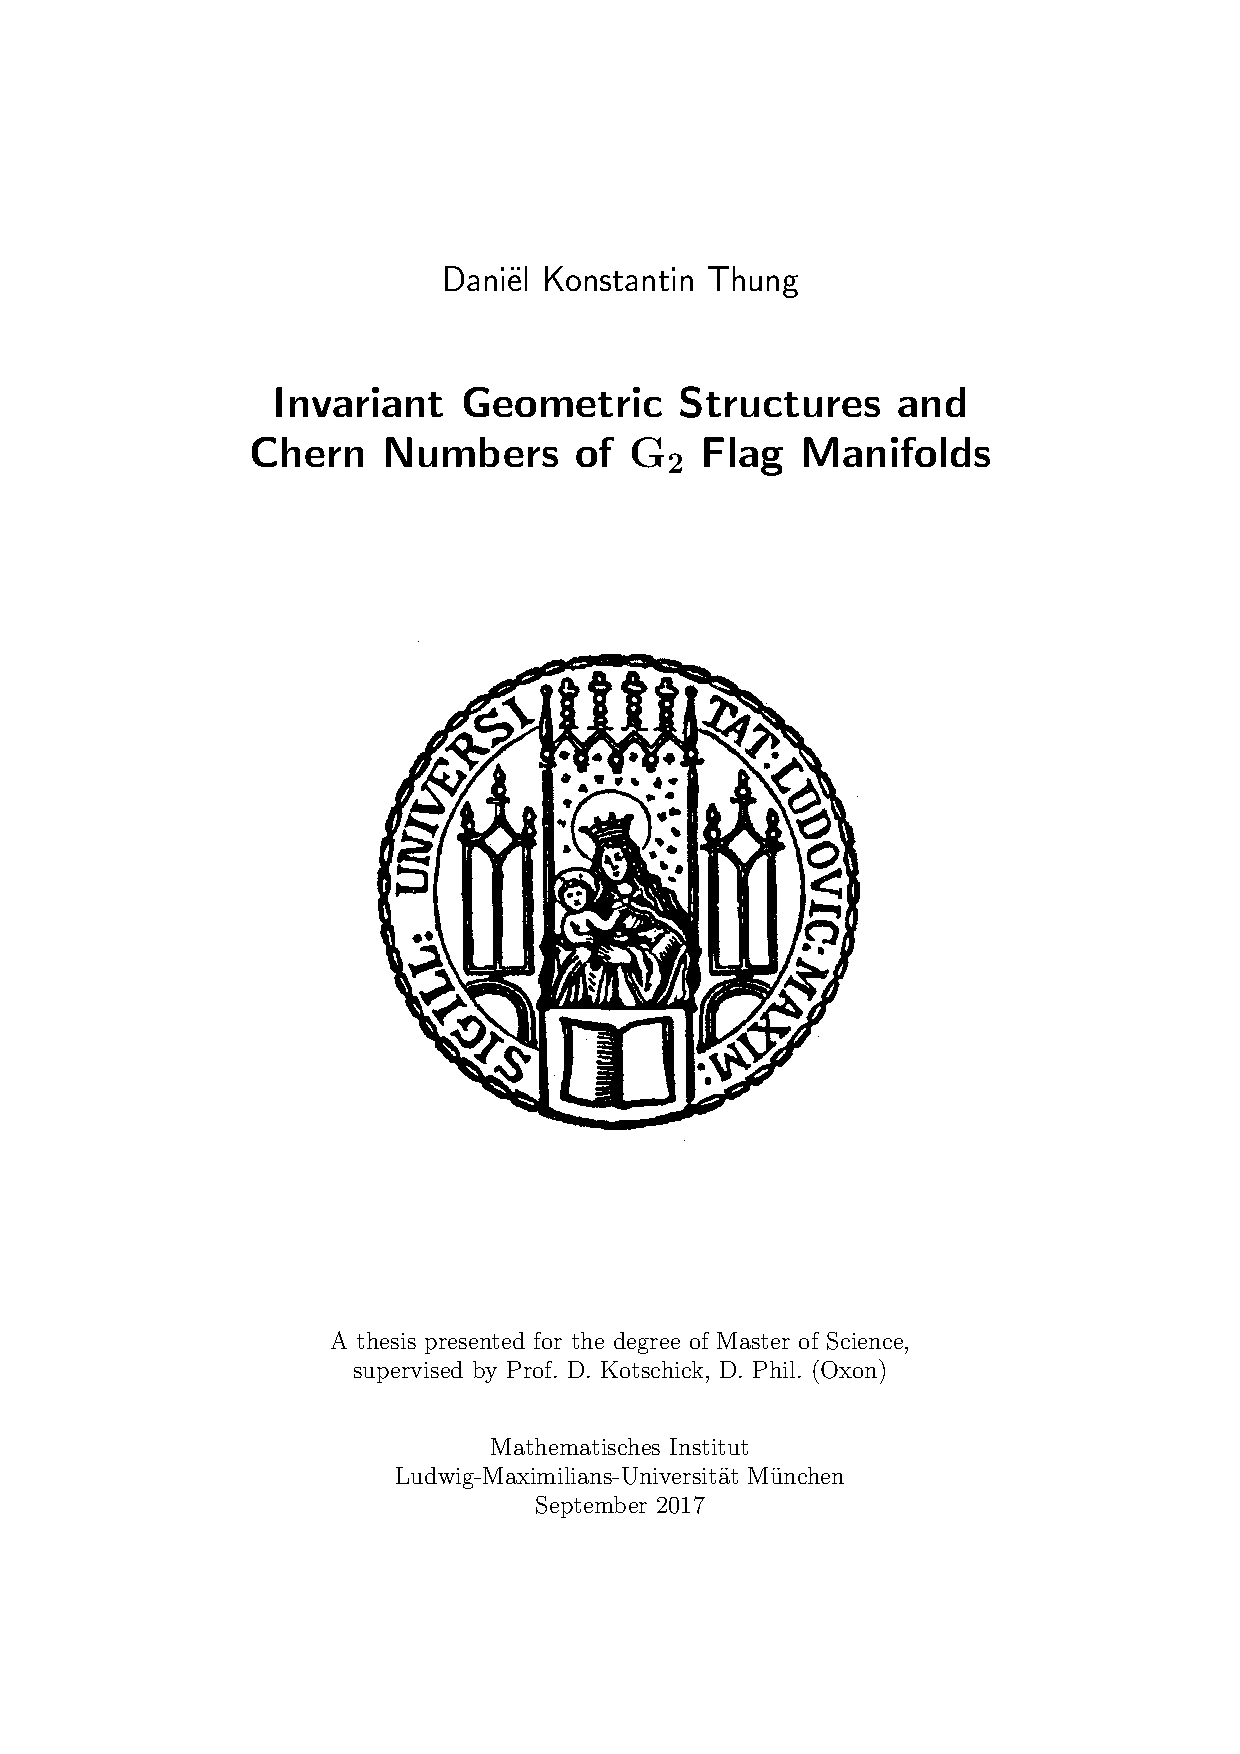
\includepdf{Chapters/titlepage}

\thispagestyle{empty} \ \clearpage 

\thispagestyle{empty}
\vspace*{4cm} 

\begin{flushright}
	To Christianna, thank you\\ 
	for your love,
	your constant encouragement\\
	and many happy days in Munich\\
\end{flushright} 
\clearpage %to make sure the main text starts on an odd page

\thispagestyle{empty} \ \clearpage 

\thispagestyle{empty} \ \clearpage
\setcounter{page}{1}

\tableofcontents

\mainmatter
\chapter{Introduction}

This thesis concerns certain manifolds that fall into the special class of homogeneous spaces known as \emph{generalized flag manifolds}. In the 1950's, it was realized that generalized flag manifolds possess remarkable properties, particularly from the point of view of complex geometry. Indeed, they are distinguished among compact, simply connected homogeneous spaces by the fact that they carry an invariant complex structure which even admits a compatible, invariant K\"ahler-Einstein metric. 

Other interesting geometric structures on generalized flag manifolds include other Einstein metrics, and almost complex structures (not necessarily integrable), which were studied by Borel and Hirzebruch in a famous series of papers. They gave a method to compute the corresponding Chern numbers and pointed out that, in some examples, the Chern numbers distinguish different invariant almost complex structures on a flag manifold. This phenomenon relates to the question of which sets of Chern numbers can be realized on a single smooth manifolds, which is of independent interest.

It is natural to study these invariant structures by means of Lie theory, leveraging the homogeneity to reduce geometric questions to algebraic ones. This has historically been the most popular approach. However, in taking it one relinquishes the use of geometric intuition, making it harder to give a concrete interpretation of the invariant geometric structures. This motivates the complementary approach taken in this work: We study certain examples of generalized flag manifolds, namely those which are homogeneous under the exceptional Lie group $G_2$, from a \emph{geometric} point of view. Avoiding the use of Lie theory, we rely on differential-geometric methods instead. 

In developing our geometric understanding of these spaces, we highlight the various branches of (almost) complex and Riemannian geometry that play a role in the study of generalized flag manifolds. In the process, we uncover surprising connections to a variety of topics ranging from the existence of complex structures on the six-sphere to rigidity theorems for K\"ahler manifolds. Our methods enable us to recover, and give an interpretation of, all the invariant almost complex structures---including the invariant K\"ahler-Einstein metric---of the manifolds we study. We then use our geometric description to compute the corresponding Chern numbers without appealing to Lie theory.

The presence of several interesting geometric structures, which interact in non-trivial ways, ensures that techniques from many different areas of mathematics find application in the study of generalized flag manifolds. By means of our detailed exposition of a few examples, we hope to convey some of its beauty to the reader.

In the first three chapters, we discuss background material. \Cref{chap:homogeneous} contains some basic information on homogeneous spaces and invariant geometric structures, while \cref{chap:twistor} is an exposition of the fundamentals of the theory of quaternionic K\"ahler manifolds, with emphasis on the associated twistor spaces. In \cref{chap:uniqueness}, we review classical rigidity theorems for the complex projective spaces and quadric hypersurfaces, in anticipation of a result that appears in \cref{chap:invarstructures}. The last two chapters are dedicated to the study of $G_2$ flag manifolds, which we introduce after discussing octonionic linear algebra in \cref{chap:flags}. The sixth and final chapter contains our main results, namely computations of the Chern numbers associated to invariant almost complex structures, as well as a rigidity theorem for one of the manifolds under consideration. 

Naturally, our choices regarding which pieces of background material to include and which to leave out reflect the prior knowledge of the author. Thus, we do not assume much background in Riemannian geometry beyond an introductory course, but nevertheless expect the reader to be familiar with the fundamentals of complex geometry and the theory of characteristic classes, as well as algebraic topology. We intend this work to be readable for geometrically-minded graduate students. 

\subsubsection{Acknowledgments}

I am greatly indebted to professor Kotschick, my supervisor, for always guiding me in the right direction, answering my questions, and shaping the way I think about mathematics. I am also grateful to Rui Coelho, who helped me get unstuck during many a tricky calculation.

I would like to thank my office mates (and our frequent office guests!), and especially Anthony, for discussions about typographical nitpicks and other daily distractions.

Finally, I want to express my gratitude to my dear friend Alex, for all the time we spent and the things we learned together. The past three years wouldn't have been the same without you.
\chapter{Homogeneous spaces and invariant geometric structures}
\label{chap:homogeneous}

In this chapter, we collect some facts from Riemannian geometry that will be of use to us, but may not be covered in standard introductory texts on the subject. We claim no originality in our discussion: This chapter largely follows parts of Besse's book on Einstein manifolds~\cite{Bes2008}, though the textbooks of Petersen~\cite{Pet2016} and Kobayashi and Nomizu~\cite{KN1963,KN1969} offer important alternatives.

\section{Homogeneous spaces}

Given a Riemannian manifold $(M,g)$ it is natural to consider its group of isometries, which we will denote by $I(M,g)$. Myers and Steenrod established the most fundamental properties of the isometry group; we recall their results without proof.

\begin{thm}[Myers-Steenrod~\cite{MS1939}]
	The isometry group $I(M,g)$ of a connected, Riemannian manifold $(M,g)$ is a Lie group acting smoothly on $M$. If $M$ is compact, then $I(M,g)$ is also compact. Furthermore, the isotropy subgroup $I_x(M,g)$ of isometries that fix $x\in M$ is closed, and the map $\rho:I_x(M,g)\to GL(T_xM)$ which sends $f$ to $\dif_x f$ defines an isomorphism onto a closed subgroup of $O(T_xM)$. Hence $I_x(M,g)$ is compact. 
\end{thm}

In this work, we study spaces on which the isometry group acts transitively.

\begin{mydef}
	A Riemannian manifold $(M,g)$ is called a \emph{(Riemannian) homogeneous space} if its isometry group $I(M,g)$ acts transitively. If $G\subset I(M,g)$ is a closed subgroup that acts transitively, we call $(M,g)$ \emph{$G$-homogeneous}. The underlying smooth manifold $M$ is called a ($G$-)homogeneous space.
\end{mydef}

When speaking about homogeneous spaces, we will typically think of the underlying smooth manifold, which may then be equipped with (possibly several distinct) metrics that turn it into a \emph{Riemannian} homogeneous space. Observe that $M$ may be $G$-homogeneous under more than one Lie group.

We also note that our definition, strictly speaking, requires the action of $G$ to be effective. However, there are many natural examples where $G$ does not effectively on a homogeneous space $M=G/H$ ($H$ is the compact isotropy subgroup of $G$). In this case, there exists a (non-trivial) normal subgroup $N$ of $H$, which may cause the isotropy representation of $H$---to be introduced shortly---to fail to be faithful. Note, however, that $G'=G/N$ still acts transitively on $G/H$, with isotropy group $H'=H/N$. Now, the action on $G/H=G'/H'$ is effective, so we may pass to this situation. In all examples of interest to us, this will not cause any problems because $G$ will always act \emph{nearly} effectively, meaning that $H$ contains at most a discrete normal subgroup $N$. Thus, passing to $G'$ will not affect the Lie-algebraic data such as the isotropy representation and we can disregard this technical point.

\begin{prop}
	Any Riemannian homogeneous space $(M,g)$is complete.
\end{prop}
\begin{myproof}
	Given any $x\in M$, there exists a closed ball $\bar B_\epsilon(0)$ of radius $\epsilon>0$ around the origin in $T_xM$ such that $\exp_x:T_xM\to M$ is defined on all of $\bar B_\epsilon(0)$. Now let $\gamma:[0,a]\to M$ be a unit speed geodesic starting at $x$. By homogeneity, there exists an isometry $\varphi\in I(M,g)$ such that $\varphi(x)=\gamma$. Then $\dif_{\gamma(a)}\varphi^{-1}(\dot \gamma(a))=v$ for some unit vector $v\in T_xM$. Set $\gamma(a+t)=\varphi(\exp_x(tX))$, $0\leq t\leq \epsilon$. This extends the original geodesic $\gamma$ by time $\epsilon$. 
\end{myproof}

Any homogeneous space $M$ is (equivariantly) diffeomorphic to a coset space $G/H$, and we will think of it as such. Here, $H$ is the stabilizer of a point in $M$; it is a closed (hence compact, since $G$ is closed) subgroup. Since for $h\in H$, left-multiplication $L_h$ fixes the coset $eH$, we have the following important representation of $H$:

\begin{mydef}
	Let $G/H$ be a homogeneous space.
	\begin{numberedlist}
		\item The \emph{(linear) isotropy representation} of $G/H$ is the homomorphism
		\begin{equation*}
			\begin{tikzcd}[row sep=-0.15cm]
				\chi: &[-32pt]H \ar[r] & GL(T_{eH}G/H)\\
				& h \ar[r,mapsto] & \dif_{eH} L_h
			\end{tikzcd}
		\end{equation*}
		\item $G/H$ is called \emph{isotropy irreducible} if $\chi$ is an irreducible representation.
	\end{numberedlist}
\end{mydef}

Let $G/H$ be a homogeneous space. If $\mf h$ denotes the Lie algebra of $H$ and $\pi:G\to G/H$ the canonical projection, then $\ker \dif_e \pi=\mf h$, hence $T_{eH}G/H\cong \mf g/\mf h$. In case $G$ is a compact Lie group, $\mf g$ admits an $\Ad_G$-invariant inner product; we then have a decomposition $\mf g=\mf h\oplus \mf m$, where $\mf m=\mf h^\perp$ is the orthogonal complement of $\mf h$ with respect to such an $\Ad_G$-invariant inner product. In particular, for any $h\in H$ we have $\Ad(h)\mf m\subset \mf m$; such a homogeneous space is called \emph{reductive}. 

Observe that, in this setting, $T_{eH}G/H\cong \mf m$: The isomorphism is given by $\dif_e\pi$. Consider the representation $\Ad_{G/H}:H\to GL(\mf m)$, obtained by restricting $\Ad_G(H)$ to $\mf m$.

\begin{prop}
	Let $G/H$ be a reductive homogeneous space. Then the isotropy representation $\chi:H\to GL(T_{eH}G/H)$ is equivalent to $\Ad_{G/H}:H\to GL(\mf m)$, i.e.~the map $\dif_e\pi\big|_{\mf m}:\mf m\to T_{eH}G/H$ is an $H$-equivariant isomorphism.
\end{prop}
\begin{myproof}
	We already know that $\dif_e\pi\big|_{\mf m}$ is a linear isomorphism, so we only need to show that for $X\in\mf m$ and $h\in H$, $\dif_e\pi(\Ad_G(h)X)=\dif_e\pi(\Ad_{G/H}(h)X)=\chi(h)(\dif_e\pi(X))$. Note that the left-hand side is well-defined because of the reductivity condition. This follows from the naturality of the exponential map:
	\begin{align*}
		\dif_e\pi(\Ad_G(h)Y)&=\od{}{t}\Big|_{t=0}\pi(\exp(t\Ad_G(h)Y))
		=\od{}{t}\Big|_{t=0}\exp(t\Ad_G(h)Y)H\\
		&=\od{}{t}\Big|_{t=0} L_h\exp(t Y) h^{-1}H
		=\dif_{eH} L_h\bigg(\od{}{t}\Big|_{t=0}\exp(tY) H\bigg)\\
		&=\chi(h)(\dif_e \pi(Y))
	\end{align*}
	This proves the claim.
\end{myproof}

Hence, we may use the representations $\chi$ and $\Ad_{G/H}$ interchangeably. Observe that, under the decomposition $\mf g=\mf h\oplus \mf m$, we have $\Ad_G(H)=\Ad_H\oplus \Ad_{G/H}$: This may be used to explicitly determine the isotropy representation in many cases.

\subsection{Symmetric spaces}

Symmetric spaces are a special kind of homogeneous spaces, which admit a geodesic-reversing ``symmetry'' around every point. They were classified in the 1920's by \'Elie Cartan, who made heavy use of the theory of Lie algebras developed by himself. We give a brief introduction here, since they will be relevant in the later chapters.

\begin{mydef}
	A connected Riemannian manifold $(M,g)$ is called a \emph{(Riemannian) symmetric space} if, for every $x\in M$, there exists an isometry $\sigma_x\in I(M,g)$ such that $\sigma_x(x)=x$ and $\dif_x \sigma_x=-\id_{T_xM}$. $\sigma_x$ is called the \emph{symmetry around $x$}.
\end{mydef}

\begin{rem}\leavevmode
	\begin{numberedlist}
		\item Since isometries on connected Riemannian manifolds are determined by their image and derivative at a single point, $\sigma_x$ is unique.
		\item Weakening the above definition by only requiring the isometries $\sigma_x$ to be locally defined (i.e.~not necessarily a global isometry), one obtains the concept of a \emph{locally symmetric space}.
	\end{numberedlist}
\end{rem}

\begin{prop}
	A symmetric space is homogeneous (and hence complete).
\end{prop}
\begin{myproof}
	We will first prove completeness directly: Let $\gamma:[0,a]\to M$ be a geodesic with $\gamma(0)=x$ and $\gamma(a)=y$. Now set $\gamma(a+t)=\sigma_y(\gamma(a-t))$ for $0\leq t\leq a$: This defines an extension of the geodesic $\gamma$.
	
	Using completeness and connectedness, we can find a geodesic connecting any two points. Then, the symmetry around the middle point (in the metric sense) of this geodesic is an isometry which interchanges the end points. Hence the isometry group acts transitively.
\end{myproof}

There are two important alternative points of view on symmetric spaces. The first of these stems from the observation that symmetric spaces have parallel curvature tensor. Indeed, for $X,Y,Z,W\in T_x M$ we have 
\begin{align*}
	\dif \sigma_x((\nabla_X R)(Y,Z)W)
	&=-(\nabla_X R)(Y,Z)W\\
	&=(\nabla_{\dif\sigma_x X}R)(\dif \sigma_x Y,\dif \sigma_x Z)\dif \sigma_x W\\
	&=(\nabla_X R)(Y,Z)W
\end{align*}
A classical theorem due to Cartan gives a precise, partial converse (see~\cite{Pet2016} or~\cite{Hel1978} for a proof).

\begin{thm}[\'{E}. Cartan]
	If a Riemannian manifold $(M,g)$ has parallel curvature tensor, then for each $x\in M$ there exists an isometry $\sigma_x$ defined on a neighborhood of $x$ such that $\sigma_x(x)=x$ and $\dif_x \sigma_x=-\id_{T_xM}$. If $(M,g)$ is simply connected and complete, then every $\sigma_x$ can be globally defined and $(M,g)$ is symmetric.
\end{thm}

Thus, Riemannian manifold with parallel curvature tensors are \emph{locally symmetric} and the Riemannian universal covering of a complete locally symmetric space is symmetric.

Finally, the structure of symmetric spaces may be encoded in terms of certain data on the Lie algebra of its isometry group. We will not try to describe this point of view here, and refer the interested reader to Helgason's classic textbook~\cite{Hel1978}. However, this point of view was the most useful for Cartan in his work on the classification of symmetric spaces.

Note that a Riemannian homogeneous space $G/H$ is symmetric as soon as we find a symmetry around a single point $gH$, since if $f$ is an isometry taking $gH$ to $g'H$, we may define $\sigma_{g'H}=f\circ \sigma_{gH} \circ f^{-1}$. For example, compact Lie groups equipped with a bi-invariant metric are symmetric: The symmetry around the identity element is simply the inversion map. 

However, compact Lie groups with bi-invariant metrics are not the only symmetric spaces. Very roughly, the classification of (simply connected) symmetric spaces can be sketched as follows (for details, see Helgason~\cite{Hel1978}). Using the Lie-algebraic description, Cartan first showed that a simply connected symmetric space decomposes as a Riemannian product of a Euclidean space with a finite number of \emph{irreducible} symmetric spaces. A symmetric space is called irreducible if its isotropy representation is irreducible. It remains to classify the simply connected, irreducible symmetric spaces.

Cartan's detailed study revealed a natural division into four types. The first two correspond to compact manifolds, while the remaining two types are non-compact. In fact, there is a duality relating the compact and non-compact types: This gives rise to the notion of a ``(non-)compact dual'' of a symmetric space. Using his own classification results on Lie groups, Cartan was able to understand all four types and produce a complete classification. Lists detailing the final results are available (for example in \cite[Ch.~10]{Hel1978}).

\section{Invariant geometric structures on homogeneous spaces}

\subsection{Invariant Einstein metrics}

Recall that on a Lie group $G$, $G$-invariant objects are described by Lie-algebraic data. This philosophy naturally generalizes to reductive homogeneous spaces $G/H$, where $G$-invariant objects correspond to $\Ad_{G/H}$-invariant objects on $\mf m$ (or $\chi$-invariant objects on $T_{eH}G/H$). We first discuss invariant metrics:

\begin{mydef}
	Let $G/H$ be a homogeneous space. A metric $g$ on $M$ is called \emph{$G$-invariant} (sometimes \emph{homogeneous}) if for every $k\in G$, left-multiplication by $k$, denoted by $L_k$, is an isometry.
\end{mydef}

Now, assume that $G/H$ is reductive (e.g.~$G$ is a compact Lie group, the case of main interest to us). Here, the above principle concretely manifests itself as follows:

\begin{prop}\label{prop:invariantmetrics}
	Let $G/H$ be a reductive homogeneous space, where $G$ has the Lie algebra $\mf g=\mf h\oplus \mf m$. Then the following objects are in bijective correspondence:
	\begin{numberedlist}
		\item $G$-invariant metrics on $G/H$.
		\item $\chi$-invariant scalar products on $T_{eH}G/H$ or equivalently $\Ad_{G/H}$-invariant scalar products on $\mf m$.
	\end{numberedlist}
\end{prop}
\begin{myproof}
	Restricting a $G$-invariant metric on $G/H$ to $eH$, we obtain an $\chi$-invariant scalar product since $L_h$ ($h\in H$) is an isometry. Conversely, if $\langle-,-\rangle$ is a $\chi$-invariant scalar product on $T_{eH}G/H$, we define a manifestly $G$-invariant metric by $g_{aH}(X,Y)=\langle \dif_a L_{a^{-1}} X, \dif_a L_{a^{-1}} Y\rangle$. This is independent of the choice of representative of $aH$, since if $b=ah$ for some $h\in H$, we have
	\begin{equation*}
		\langle \dif_b L_{b^{-1}} X,\dif_b L_{b^{-1}} Y\rangle
		=\langle \dif_{ah} L_{h^{-1}a^{-1}} X,\dif_{ah} L_{h^{-1}a^{-1}} Y\rangle
		=\langle \dif_a L_{a^{-1}} X,\dif_a L_{a^{-1}} Y\rangle
	\end{equation*}
	by $\chi$-invariance.
\end{myproof}

The most important takeaway is that the Riemannian data of $G/H$, equipped with a $G$-invariant metric, are determined by the associated $\Ad_{G/H}$-invariant inner product on $\mf m$, together with the Lie algebraic data of $\mf g$. The invariance of the curvature tensor under isometries means it is determined by its value at $eH$. By the same token, the fact that $H$ acts by isometries implies that the curvature is $\chi$-invariant.

Now consider a homogeneous space $G/H$, where $G$ is compact and semisimple. Then the Killing form $B$ on $\mf g$ is an $\Ad_G$-invariant scalar product on $\mf g$, and we identify $T_{eH}G/H\cong \mf m$, where $\mf m=\mf h^\perp$ is the orthogonal complement of $\mf h$ with respect to $B$. We have seen that $G$-invariant metrics correspond to inner products on $\mf m$ invariant under the isotropy representation. 

Decompose $T_{eH}G/H\cong \mf m$ into irreducible summands under the isotropy representation: $\mf m=\mf m_1\oplus\dots\oplus \mf m_s$. If the $\mf m_j$ are pairwise non-equivalent, then this decomposition is unique. This is the case of interest to us. By a variant of Schur's lemma, the restriction of an invariant inner product to a summand $\mf m_j$ must be a multiple of (minus) the Killing form, restricted to $\mf m_j$:

\begin{lem}\label{lem:Schurscalarproducts}
	Let $\rho:G\to GL(V)$ be an irreducible representation. Then any two $\rho$-invariant scalar products on $V$ are proportional.
\end{lem}
\begin{myproof}
	Let $\langle -,-\rangle_i$, $i=1,2$ be $\rho$-invariant scalar products and define $g_i:V\to V^*$ by $v\mapsto \langle v,-\rangle_i$. Now set $L=g_2^{-1}\circ g_1$. This linear map is easily seen to be symmetric with respect to the inner products and $\rho$-equivariant, hence its eigenspaces are $\rho$-invariant. Irreducibility then implies that $L=\lambda\cdot \id_V$ for some $\lambda\in \R$.
\end{myproof}

\begin{rem}
	Actually, if $\langle -,-\rangle$ is an invariant scalar product and $A$ is an invariant, symmetric bilinear form, the exact same proof goes through to show that $A$ is proportional to $\langle-,-\rangle$, if one defines $a:V\to V^*$, $v\mapsto A(v,-)$ and sets $L=g^{-1}\circ a$. 
\end{rem}

Hence, in the above setup, homogeneous metrics are in bijective correspondence with inner products of the form
\begin{equation}\label{eq:diagonalKillingmetrics}
	\langle \ \ ,\ \, \rangle =x_1(-B)|_{\mf m_1}+\dots+x_s(-B)|_{\mf m_s} 
	\qquad \qquad x_j>0\ \ \ \forall j
\end{equation}
Such $G$-invariant metrics, which are called \emph{diagonal}, are determined by the positive constants $x_1,x_2,\dots,x_s$. In particular, if $G/H$ is isotropy irreducible, then it admits a unique $G$-invariant metric, up to homothety.

$G$-invariant metrics are privileged, but not as privileged as $G$-invariant \emph{Einstein} metrics.

\begin{mydef}
	A Riemannian manifold $(M,g)$ is called \emph{Einstein} if $r_g=\lambda g$ for some constant $\lambda\in \R$, where $r_g$ denotes the Ricci curvature of $g$.
\end{mydef}

\begin{rem}
	Let $M$ be a compact manifold. It has been known since 1915 that Einstein metrics are precisely the critical points of the total scalar curvature functional
	\begin{equation*}
	S(g)=\int_M s_g \vol_g
	\end{equation*}
	This fact, due to Hilbert, is used to formulate the variational approach to Einstein's theory of general relativity (physicists call this functional the \emph{Einstein-Hilbert action}). This explains why these manifolds are called \emph{Einstein}.
\end{rem}

Wolf observed that, if the isotropy representation is irreducible, invariant metrics are automatically Einstein:

\begin{prop}[Wolf,~\cite{Wol1968}]
	If $G/H$ is an isotropy irreducible homogeneous space, then $G/H$ admits a unique (up to homothety) $G$-invariant metric, which is Einstein.
\end{prop}
\begin{myproof}
	We have already established that all $G$-invariant metrics are proportional in this case; pick one of them an denote the induced inner product on $T_{eH}G/H$ by $\langle -,-\rangle$. The Ricci curvature corresponds to a $\chi$-invariant, symmetric bilinear form on $T_{eH}G/H$ and therefore must also be proportional to $\langle -,-\rangle$. By homogeneity, they must be proportional at every point.
\end{myproof}

This is certainly the simplest situation, but in other special cases $G$-invariant Einstein metrics can be studied directly as well. For instance, Wang and Ziller~\cite{WZ1985} considered so-called \emph{standard} homogeneous spaces. These are homogeneous spaces $G/H$ ($G$ compact, connected and semisimple) equipped with the $G$-invariant metric derived from the Killing form on $G$. In this simple and natural case, they were able to determine the necessary and sufficient condition for the standard homogeneous metric to be Einstein, using Lie-algebraic methods. 

In~\cite{WZ1986a} (see also the follow-up paper~\cite{BWZ2004}), Wang and Ziller approached the problem from a different angle, outlining a variational approach for general compact homogeneous spaces based on the characterization of Einstein metrics as critical points of the total scalar curvature functional. Restricting this functional, which we called $S$ before, to the space $\ms M_G^1$ of $G$-invariant metrics of volume $1$, $s_g$ is constant and equal to $S(g)$; the critical points are exactly the $G$-invariant Einstein metrics.

Decompose $T_{eH}G/H$ into isotropy irreducible summands $\mf m_i$. As mentioned before, we are primarily interested in the case where this decomposition is unique. Then all $G$-invariant metrics are diagonal with respect to this decomposition, i.e.~given by $\chi$-invariant inner products on of the form
\begin{equation*}
	Q=x_1 Q\big|_{\mf m_1}+\dots+ x_s Q\big|_{\mf m_s}\qquad \qquad x_j>0\ \ \forall j
\end{equation*}
In this setup, Wang and Ziller give an explicit, algebraic expression for the scalar curvature in terms of Lie-algebraic data of $\mf m$. This formula and its extensions were used by several authors to classify $G$-invariant Einstein metrics in many examples where the isotropy representation has only a few irreducible summands, when the equations are algebraically tractable (e.g.~\cite{Ker1996,PS1997,DK2008}). This includes many ``generalized flag manifolds'', which will be the focus of this work (see \cref{chap:flags,chap:invarstructures}).

If one is interested in Einstein metrics in general, without necessarily requiring invariance, then there are several other approaches. One of them, which will be relevant to us later, uses the theory of so-called Riemannian submersions. In particular, the notion of ``canonical variation'' gives an efficient way of generating new Einstein metrics from old ones; this procedure also preserves invariance and can therefore be applied to obtain new invariant Einstein metrics from a given one. We have given a brief account of this framework, which will also be of use in \cref{chap:twistor}, in \cref{app:submersions}.

\subsection{Invariant almost complex structures}

The invariant objects that take center stage in this work are not metrics, but almost complex structures. Here, we immediately give the definition in terms of data on $T_{eH}G/H$ instead of giving a ``global'' definition (in terms of a $G$-invariant tensor field on $G/H$) and showing equivalence:

\begin{mydef}
	An almost complex structure $J$ on a homogeneous space $G/H$ is called \emph{$G$-invariant} if $J_{eH}$ commutes with the isotropy representation.
\end{mydef}

The study of invariant complex structures for specific classes of manifolds was initiated in the 1950's with papers by Wang, Koszul and Borel~\cite{Wan1954,Kos1955,Bor1954}; in \cref{chap:flags} we will discuss some of their results, in particular those concerning generalized flag manifolds.

Not long after these pioneering works, Borel and Hirzebruch published a series of seminal papers, in which they gave a comprehensive treatment of invariant almost complex structures on general homogeneous spaces~\cite{BH1958a}. Their results include a recipe to enumerate invariant almost complex structures, a criterion for integrability and a method to compute characteristic classes in terms of purely Lie-algebraic data associated to the homogeneous space. They also gave many applications, often to generalized flag manifolds.

As mentioned in the introduction, our aim in this work is to \emph{avoid} the Lie-theoretic framework and to give a more geometric treatment of certain examples which may alternatively be investigated by the methods of Borel and Hirzebruch. Therefore, we will not give an extended discussion of their results here. For a succinct summary of their treatment of generalized flag manifolds, we refer to Kotschick and Terzi\'c's paper~\cite[Sec.~2]{KT2009}. 

We describe only one piece of information, namely how to enumerate invariant almost complex structures (cf.~\cite[\S 13.4--5]{BH1958a}); this will be useful to us later. Consider a homogeneous space $G/H$ which we assume admits at least one invariant almost complex structure. Decompose $T_{eH}G/H=\mf m_1\oplus\dots \oplus \mf m_k$ into irreducible summands under the isotropy representation. Then invariant almost complex structures must respect this decomposition, and the restrictions of any two invariant almost complex structures $J_1$, $J_2$ to $\mf m_j$ must be equal up to conjugation. This follows from a variant of Schur's lemma: Mimicking the proof of \cref{lem:Schurscalarproducts} on the complexification of $T_{eH}G/H$ (to ensure that $J_2^{-1}\circ J_1$ has an eigenvalue, which must be $\pm 1$) and restricting to the conjugation-invariant (i.e.~real) subspace shows that $J_2^{-1}\circ J_1=\pm \id_{T_{eH}G/H}$, which proves the claim. 

Hirzebruch and Borel prove that each summand $\mf m_j$ indeed admits exactly one almost complex structure up to conjugation. Thus, $k$ irreducible summands give rise to $2^{k-1}$ distinct invariant almost complex structures, after identifying conjugate structures. This result applies to the spaces we focus on in this work, i.e.~generalized flag manifolds, since these always admit an invariant (almost) complex structure (see \cref{chap:flags}).
\chapter{Quaternionic K\"ahler manifolds and twistor spaces}
\label{chap:twistor}

In this chapter, we discuss quaternionic K\"ahler manifolds and their \emph{twistor spaces}. There are a number of distinct approaches to this topic, corresponding to different motivations for studying quaternionic K\"ahler manifolds. We will roughly follow the discussion of Salamon in~\cite{Sal1982}, though some of the proofs are taken from~\cite{Bes2008} (again, we claim no originality). For alternative points of view, see for instance~\cite{BO1984,Sal1984,Sal1986} and the review~\cite{Sal1999}. Quaternionic K\"ahler manifolds have also attracted attention from physicists in the context of supergravity theories (see for instance the original reference~\cite{BW1983} or the recent book~\cite{Cor2010}). However, we will not investigate the connections to physics in this work.

\section{What is a quaternionic K\"ahler manifold?}

The classification of holonomy groups provides one of the motivations for studying quaternionic K\"ahler manifolds. To explain this, we will briefly discuss (without proofs) a few important results regarding holonomy groups; details can be found in~\cite{KN1963,Bes2008,Joy2000a}. Recall that the holonomy group of a connected Riemannian manifold $(M,g)$, denoted by $\Hol(g)$, is the compact (this is a theorem!) Lie subgroup of $O(T_pM)$ generated by parallel transport along all loops based at $p\in M$. Since changing the base point yields a conjugate subgroup, the choice of base point is immaterial (we will henceforth speak implicitly about conjugacy classes of subgroups). Restricting to null-homotopic loops yields the \emph{restricted} holonomy group $\Hol^0(g)$.

According to whether the holonomy representation on the tangent spaces is reducible or not, we call $(M,g)$ reducible or irreducible. In the former case, one obtains two complementary subbundles of $TM$. They are integrable (in the sense of Frobenius' theorem) and one may prove that $M$ is then locally isometric to a Riemannian product. If there is a subbundle on which $\Hol(g)$ acts trivially, then the corresponding integral manifold is locally isometric to a Euclidean space. From now on, we will assume that $M$ is complete. Then, after possibly passing to the universal covering space $(\tilde M,\tilde g)$, a famous theorem due to De Rham yields a unique way to decompose it into irreducible manifolds:

\begin{thm}[De Rham, {\cite[Sec. IV.6]{KN1963}}]
	A connected, simply connected, complete, reducible Riemannian manifold is isometric to a Riemannian product of connected, simply connected and complete Riemannian manifolds.
\end{thm}

Proceeding inductively, one finds:

\begin{thm}[De Rham Decomposition Theorem]
	A connected, simply connected, complete Riemannian manifold is isometric to a Riemannian product of connected, simply connected, complete and irreducible Riemannian manifolds with a Euclidean space (possibly of dimension zero). This decomposition is unique up to order.
\end{thm}

When studying the \emph{restricted} holonomy group, one can work under the assumption of simple connectedness without loss of generality. Indeed, null-homotopic loops based at $p$ are precisely the images of loops in the universal covering $(\tilde M,\tilde g)$ (based at a fixed lift of $p$), hence $\Hol^0(g)=\Hol^0(\tilde g)=\Hol(\tilde g)$.

In the early twentieth century, \'Elie Cartan succeeded in classifying the irreducible, simply connected symmetric spaces and computing their holonomy groups. Recall from \cref{chap:homogeneous} that symmetric spaces are Riemannian homogeneous spaces, i.e.~of the form $M\cong G/H$ where $G$ is a Lie group and $H$ a compact subgroup. It follows from Cartan's classification that, although $M$ may be homogeneous under different groups, there is only one combination $(G,H)$ (called a \emph{symmetric pair}) which turns $M$ into a symmetric space. It turns out that the holonomy group is given by the isotropy group $H$ itself. By our above remark, this determines the restricted holonomy groups of locally symmetric spaces. 

This begs the question: What about the holonomy of Riemannian manifolds which are \emph{not} locally symmetric? That question was answered by Berger in 1955:

\begin{thm}[Berger, {\cite{Ber1955}}]
	Let $(M,g)$ be a complete, connected, simply connected and irreducible Riemannian manifold which is not symmetric. Then its holonomy group occurs in the following list:
	\begin{center}
		\begin{tabular}{llll} \toprule
			Dimension				& Holonomy Group		\\ \midrule
			$n$ 					& $SO(n)$				\\
			$n=2m,\ m\geq 2$ 		& $U(m)$				\\
			$n=2m,\ m\geq 2$		& $SU(m)$ 				\\
			$n=4m,\ m\geq 2$		& $Sp(m)\cdot Sp(1)$	\\
			$n=4m,\ m\geq 2$		& $Sp(m)$				\\
			$n=8$					& $\Spin(7)$			\\
			$n=7$					& $G_2$					\\ \bottomrule
		\end{tabular}
	\end{center}
	where $Sp(m)\cdot Sp(1)=(Sp(m)\times Sp(1))/\Z_2$, where $(\pm \id,\pm 1)$ are identified.
\end{thm}

\begin{rem}\leavevmode
	\begin{numberedlist}
		\item The original list of Berger included the case $n=16$, with holonomy group $\Spin(9)$. Alekseevski\u{\i}~\cite{Ale1967} showed that such a manifold is always locally symmetric. A few years later, Brown and Gray~\cite{BG1972} gave an independent proof of this fact.
		\item $SO(n)$, the largest holonomy group, is known as the ``generic'' case; any oriented Riemannian manifold has holonomy group contained in $SO(n)$. Among the reduced holonomy groups, the most famous case is the group $U(m)$: This corresponds to K\"ahler manifolds. The inclusions of $SU(2m)$ and $Sp(m)$ into $U(2m)$ show that the corresponding manifolds, called Calabi-Yau and hyper-K\"ahler, respectively, are special types of K\"ahler manifolds.
		\item Besides giving the holonomy group, one should really specify how it acts. One may then observe that the above actions are always transitive on the unit spheres in the tangent spaces. This fact has been the focus of a lot of attention; direct proofs have been provided by Simons~\cite{Sim1962} and more recently Olmos~\cite{Olm2005}, whose proof is geometric (rather than algebraic) in nature.
	\end{numberedlist} 
\end{rem}

It is natural to expect, for instance by taking inspiration from the K\"ahler case, that each possible holonomy group corresponds to a distinct ``flavor'' of geometry. This provides a strong motivation for studying the geometric structures that arise for each holonomy group. Furthermore, Berger did not address the natural question whether there actually exist manifolds whose (global!) holonomy groups coincide with the groups that appear in his list. It took thirty more years to prove that this is indeed the case and there is considerable interest in constructing new examples, which are often relatively scarce. Thus, one is naturally led to study the following class of manifolds:

\begin{mydef}
	A quaternionic K\"ahler manifold $(M,g)$ is an (oriented) manifold of dimension $4n$, $n\geq 2$, whose holonomy group is contained in $Sp(n)\cdot Sp(1)$.
\end{mydef}

The case $n=1$ is excluded because $Sp(1)\cdot Sp(1)\cong SO(4)$. To see this, observe that $Sp(1)\cong SU(2)$. Indeed, under the standard identification of $\H$ with $\C^2$, right-multiplication with a unit quaternion $q=a+bi+cj+dk$ (where $a^2+b^2+c^2+d^2=1$) corresponds to left-multiplication by 
$\begin{psmallmatrix}
	a+bi & -c+di \\ c+di & a-bi
\end{psmallmatrix}$, which is precisely the general form of an element of $SU(2)$. Now, our assertion follows from the well-known fact that $(SU(2)\times SU(2))/\Z_2\cong SO(4)$.

More generally, $Sp(n)\cdot Sp(1)$ is realized as a subgroup of $SO(4n)$ as follows: Consider $\R^{4n}$ as a right $\H$-module by identifying it with $\H^n$, on which $\H$ acts from the right. The action of the unit quaternions then induces an embedding of $Sp(1)$ into $SO(4n)$. We identify $GL(n,\H)$ with the subgroup of $GL(2n,\C)$ formed by block-matrices of the form 
$\begin{psmallmatrix}
	A & -\bar B \\ B & \bar A
\end{psmallmatrix}$. Since $Sp(n)$ is defined as those elements of $GL(n,\H)$ that preserve the standard (symplectic) inner product on $\H^n$, which corresponds to that of $\C^{2n}$ under the natural identification, we see that $Sp(n)\subset U(2n)$. 

In fact, $Sp(n)\subset SU(2n)$; this is easiest seen by noting that elements of its Lie algebra are automatically traceless and skew-Hermitian. Thus, after embedding $SU(2n)$ into $SO(4n)$, we also obtain an embedding of $Sp(n)$ into $SO(4n)$. The image is the subgroup of $SO(4n)$ that commutes with the image of the embedding of $Sp(1)$, since it is precisely these elements that come from $\H$-linear maps. Abusing notation, we identify $Sp(1)$ and $Sp(n)$ with their images in $SO(4n)$ and form the product $Sp(n)\cdot Sp(1)$, which is easily seen to be isomorphic to $(Sp(n)\times Sp(1))/\Z_2$.

\begin{rem}\leavevmode
	\begin{numberedlist}
		\item The name ``quaternionic K\"ahler manifold'' suggests that these manifolds are the quaternionic analogs of K\"ahler manifolds. This may initially sound surprising, since the naive quaternionic analog of $U(n)$-holonomy is $Sp(n)$-holonomy. However, the inclusion $Sp(n)\subset SU(2n)$ shows that such (hyper-K\"ahler) manifolds  are even Calabi-Yau, and thus correspond to a very special subclass of K\"ahler manifolds.
		
		The analogy with $Sp(n)\cdot Sp(1)$, which includes hyper-K\"ahler manifolds as a special case, is better: Indeed, we will soon encounter a four-form $\Omega$ which plays a role similar to that of the K\"ahler form. Moreover, we will shortly see that there is a natural way to associate a complex manifold to a quaternionic K\"ahler manifold, which is in some cases even K\"ahler, so that K\"ahler geometry plays a role in the theory as well.
		\item The reader should be warned that, despite this analogy and the name, quaternionic K\"ahler manifolds are not complex or even \emph{almost} complex in general, let alone K\"ahler. Consider the quaternionic projective spaces $\HP^n\cong (Sp(n+1)/\Z_2)/Sp(n)\cdot Sp(1)$, which are symmetric spaces. This means that they have holonomy $Sp(n)\cdot Sp(1)$ and hence are quaternionic K\"ahler. However, it can be shown using characteristic classes that $\HP^n$ cannot be almost complex for any $n\in\N$~\cite{Hir1960,Mas1962}.
	\end{numberedlist}
\end{rem}

To understand the connection between quaternionic geometry and holonomy $Sp(n)\cdot Sp(1)$ more clearly, we first have to do some linear algebra (following Kraines~\cite{Kra1966}). Consider $\H^n$ as a right-module over $\H$ and recall the symplectic inner product which sends $P, Q\in \H^n$ to $\langle P,Q\rangle \coloneqq \sum_{a=1}^n p_a \bar q_a$. 

Now define a new inner product $(P,Q)\coloneqq \frac{1}{2}(\langle P,Q\rangle +\langle Q,P\rangle )$ (which will correspond to a Riemannian metric) and the three two-forms 
\begin{equation*}
	\Omega_I(P,Q)\coloneqq (P i,Q) \qquad \qquad 
	\Omega_J(P,Q)\coloneqq (P j,Q) \qquad \qquad 
	\Omega_K(P,Q)\coloneqq (P k,Q)
\end{equation*}
It is clear that $i^*\Omega_I=\Omega_I=\Omega_I$, $j^*\Omega_J=\Omega_J$ and $k^*\Omega_K=\Omega_K$ (remember that $i,j,k$ act by right-multiplication). More generally, a (tedious) computation shows:

\begin{lem}\label{lem:QKcovderivs}
	Let $\lambda=a+bi+cj+dk\in Sp(1)$. Then
	\begin{align*}
		\lambda^*\Omega_I&=(a^2+b^2-c^2-d^2)\Omega_I+2(ad+bc)\Omega_J
		+2(bd-ac)\Omega_K\\
		\lambda^*\Omega_J&=2(bc-ad)\Omega_I+(a^2-b^2+c^2-d^2)\Omega_J
		+2(ab+cd)\Omega_K\\
		\lambda^*\Omega_K&=2(ac+bd)\Omega_I+2(cd-ab)\Omega_J
		+(a^2-b^2-c^2+d^2)\Omega_K
	\end{align*}
\end{lem}

Now, we define the four-form $\Omega=\Omega_I\wedge \Omega_I+\Omega_J\wedge\Omega_J+\Omega_K\wedge\Omega_K$. The above lemma guarantees that $\lambda^*\Omega=\Omega$. $Sp(n)$-invariance of the inner product $\langle-,-\rangle$ shows that $\Omega$ is in fact $Sp(n)\cdot Sp(1)$-invariant. 

Now, starting from a quaternionic K\"ahler manifold, we may identify its tangent space over a given point with $\H^n$. This identification will in general not be preserved when passing to a different chart with overlapping domain, but since we may choose the transition functions to take values in $Sp(n)\cdot Sp(1)$ the form $\Omega$ (initially defined with respect to a specific identification) is well-defined. Moreover, $Sp(n)\cdot Sp(1)$-invariance shows that $\Omega$ is invariant under parallel transport along any loop, so we obtain:

\begin{prop}
	A quaternionic K\"ahler manifold admits a non-vanishing, parallel four-form. \proofclear
\end{prop}

In fact, with a little more effort one may prove that $\Omega$ is non-degenerate and use this in the study of the cohomology of $M$; one immediate corollary is that the Betti numbers $b_{4n}(M)$ are nonzero since any parallel form (such as $\Omega^n$) is closed and co-closed. Other applications include an analog of the Lefschetz decomposition on K\"ahler manifolds (see~\cite{Kra1966}). 

In the differential-geometric setting, \cref{lem:QKcovderivs} means that a quaternionic K\"ahler manifold locally admits three two-forms $\Omega_{I,J,K}$ whose covariant derivatives are linear combinations of $\Omega_{I,J,K}$ at each point. Since the Levi-Civit\`a connection is compatible with the metric, $(\nabla_X\Omega_I)(Y,Z)=g((\nabla_X R_I)Y,Z)$, where $R_I$ is the endomorphism (locally defined!) that corresponds to right-multiplication by $i\in \H$. 

Thus, we may equivalently say that the covariant derivatives of $R_{I,J,K}$ can be expressed in terms of the $R_{I,J,K}$ themselves, i.e.~the three-dimensional bundle of endomorphisms they span is preserved by covariant differentiation. This shows that quaternionic K\"ahler manifolds can be equipped with a covering by special charts (in the following, we identify $R_{I,J,K}$ with $I$, $J$, $K$):

\begin{prop}\label{prop:QKcharts}
	A quaternionic K\"ahler manifold $(M,g)$ admits an open covering $\{U_i\}$ with the following properties:
	\begin{numberedlist}
		\item On each $U_i$, there exist two almost complex structures $I$ and $J$ such that $IJ=-JI$.
		\item On $U_i$, $g$ is Hermitian with respect to $I$ and $J$ defined with respect to $U_i$.
		\item The covariant derivatives of $I$ and $J$ are (pointwise) linear combinations of $I$, $J$ and $K=IJ$.
		\item For every $x\in U_i\cap U_j$, the subspace of $\End(T_xM)$ spanned by $I$, $J$ and $K$ is independent of whether $I$ and $J$ are defined with respect to $U_i$ or $U_j$. In other words, they define a three-dimensional subbundle of $\End TM$.
	\end{numberedlist}
\end{prop}
\begin{myproof}
	The first three points follow from out discussion above. The final point is a consequence of the fact that $Sp(n)\cdot Sp(1)\subset SO(4n)$ preserves (under conjugation) the vector subspace of endomorphisms of $\R^{4n}=\H^n$ generated by multiplication by $i,j,k$. To see this, let $L\in Sp(n)\cdot Sp(1)$ be given by $v\mapsto (Av)q$, where $A\in Sp(n)$, $q\in Sp(1)$. Now let $p\in \Im \H$ (acting from the right); then $L^{-1}\circ p\circ L(v)=vq^{-1}pq$. Since $q^{-1}pq\in \Im\H$, $Sp(n)\cdot Sp(1)$ indeed preserves the subspace of endomorphisms induced by $\Im\H$.
\end{myproof}

\begin{rem}\leavevmode
	\begin{numberedlist}
		\item In fact, it is possible to prove (though we will not do so) that a manifold that admits such a covering must be quaternionic K\"ahler, thus providing an alternative characterization of quaternionic K\"ahler manifolds.
		\item Using the quaternionic relations between $I$, $J$ and $K$ we find that the third condition is equivalent to the existence of locally defined one-forms $\alpha$, $\beta$ and $\gamma$ such that:
		\begin{align*}
			\nabla_X I&= \alpha(X)J - \beta(X)K\\
			\nabla_X J&= -\alpha(X)I + \gamma(X)K\\
			\nabla_X K&= \beta(X)I - \gamma(X)J
		\end{align*}
		To see that $\nabla_X I$ has no term proportional to $I$ (and the same holds for $J$, $K$), one must consider $\nabla_X (I^2)=0$ and work out the left-hand side using the Leibniz rule. The relations between the coefficient one-forms are determined in analogous fashion, starting from $\nabla_X(JK)=\nabla_X I$ and its cyclic permutations.
	\end{numberedlist}
\end{rem}

Reduced holonomy typically implies heavy restrictions on curvature. In fact, of the holonomy groups that appear in Berger's list, $U(m)$ and $Sp(m)\cdot Sp(1)$ are the only ones that allow for manifolds that are \emph{not} necessarily Ricci-flat. However, for quaternionic-K\"ahler manifold we do have the following:

\begin{thm}[Berger,~\cite{Ber1966}\footnote{We were unable to consult this source in person; the theorem is credited to this paper by several independent sources.}]
	Every quaternionic K\"ahler manifold is Einstein.
\end{thm}
\begin{myproof}
	We reproduce the elementary proof due to Ishihara~\cite{Ish1974} (see also~\cite{Bes2008}). Since the Einstein condition is local, we may work inside one of the charts from \cref{prop:QKcharts}. Using $R(X,Y)=\nabla_X\nabla_Y-\nabla_Y\nabla_X-\nabla_{[X,Y]}$ and the above expression for $\nabla_X I$, we find:
	\begin{align*}
		[R(X,Y),I]
		&=\big(\nabla_X(\nabla_Y I)-\nabla_Y(\nabla_X I)-\nabla_{[X,Y]}I\big)\\
		&=\big(\d(\alpha(Y))(X)-\d(\alpha(X))(Y)-\alpha([X,Y])\big)J\\
		&\,-\big(\d(\beta(Y))(X)-\d(\beta(X))(Y)-\beta([X,Y])\big)K\\
		&\,+\alpha(Y)\nabla_X J-\alpha(X)\nabla_Y J
		-\beta(Y)\nabla_X K+\beta(X)\nabla_Y K
	\end{align*}
	The terms featuring covariant derivatives of $J$ and $K$ cancel, so we find that 
	\begin{equation}\label{eq:Icurvcommutator}
		[R(X,Y),I]=\alpha(X,Y)J-\beta(X,Y)K
	\end{equation}
	where $\alpha(X,Y)\coloneqq \d(\alpha(Y))(X)-\d(\alpha(X))(Y)-\alpha([X,Y])$ is a two-form and $\beta$ is defined analogously. In similar fashion, one finds that
	\begin{align}\label{eq:Jcurvcommutator}
		[R(X,Y),J]&=-\alpha(X,Y) I+\gamma(X,Y) K\\\label{eq:Kcurvcommutator}
		[R(X,Y),K]&=\beta(X,Y) I-\gamma(X,Y) J
	\end{align}
	Now we need a computational lemma: 
	
	\begin{lem}\label{lem:ricciforms}
		The forms $\alpha$, $\beta$, $\gamma$ are related to the Ricci curvature $r$ via:
		\begin{align*}
			\alpha(X,Y)=\frac{1}{n+2}r(KX,Y)\\ 
			\beta(X,Y)=\frac{1}{n+2}r(JX,Y)\\
			\gamma(X,Y)=\frac{1}{n+2}r(IX,Y)
		\end{align*}
		where $n=\dim M/4$.
	\end{lem}
	\begin{myproof}[Proof of Lemma]
		Starting from \eqref{eq:Kcurvcommutator}, we have:
		\begin{align*}
			g([R(X,Y),K]Z,JZ)&=
			g(\beta(X,Y)IZ,JZ)-g(\gamma(X,Y)JZ,JZ)\\
			&=-\gamma(X,Y)\lvert Z\rvert^2
		\end{align*}
		Using the quaternionic relations and the symmetries of $R$ on the left-hand side, this becomes
		\begin{equation}\label{eq:gammacurvrelation}
			g(R(X,Y)JZ,KZ)+g(R(X,Y)Z,IZ)=\gamma(X,Y)\lvert Z\rvert^2
		\end{equation}
		Now we pick a local orthonormal basis $\{X_i\}$ of $TM$, adapted to the quaternionic coordinates in the sense that if $X_i$ is a basis element, then $IX_i$, $JX_i$ and $K X_i$ are too (up to sign). This means that the set of pairs $(X_i,IX_i)$ is at the same time the set of pairs $(JX_i,KX_i)$; the above identity for $Z=X_i$ yields, when summed over $i$, the identity
		\begin{equation*}
			2n\gamma(X,Y)=\sum_{i=1}^{4n}g(R(X,Y)X_i,IX_i)
		\end{equation*}
		The first Bianchi identity applied to the last three entries of the right-hand side yields
		\begin{align*}
			2n\gamma(X,Y)
			&=\sum_{i=1}^{4n}\Big(g(R(X,X_i)Y,IX_i)-g(R(X,IX_i)Y,X_i)\Big)
		\end{align*}
		Both terms contribute equally so we find
		%WORK NEEDED: Why?
		\begin{equation*}
			n\gamma(X,Y)=\sum_ig(R(X,X_i)Y,IX_i)=-\sum_i g(IR(X,X_i)Y,X_i)
		\end{equation*}
		Now we can use \eqref{eq:Icurvcommutator}:
		\begin{align*}
			n\gamma(X,Y)&=\sum_i\Big(-g(R(X,X_i)IY,X_i)+\alpha(X,X_i)g(JY,X_i)
			-\beta(X,X_i)g(KY,X_i)\Big)\\
			&=-r(X,IY)+\alpha(X,JY)-\beta(X,KY)
		\end{align*}
		Replacing $Y$ by $IY$, this means that
		\begin{equation*}
			n\gamma(X,IY)+\beta(X,JY)+\alpha(X,KY)=r(X,Y)
		\end{equation*}
		Carrying out identical calculations for cyclic permutations of $\{I,J,K\}$, one obtains
		\begin{align*}
			\gamma(X,IY)+n\beta(X,JY)+\alpha(X,KY)=r(X,Y)\\
			\gamma(X,IY)+\beta(X,JY)+n\alpha(X,KY)=r(X,Y)
		\end{align*}
		Since $n\geq 2$, this suffices to conclude that
		\begin{equation*}
			\gamma(X,IY)=\beta(X,JY)=\alpha(X,KY)=\frac{1}{n+2}r(X,Y)
		\end{equation*}
		from which the claim easily follows.
	\end{myproof}
	Now it is not hard to finish the proof of the theorem. Note that
	\begin{equation*}
		r(X,Y)=r(IX,IY)=r(JX,JY)=r(KX,KY)
	\end{equation*}
	and therefore, using \eqref{eq:gammacurvrelation}, we find:
	\begin{align*}
		\frac{2\lvert Z\rvert^2}{n+2}r(X,X)
		&=\frac{\lvert Z\rvert^2}{n+2}(r(X,X)+r(JX,JX))\\
		&=g(R(X,IX)Z,IZ)+g(R(X,IX)JZ,KZ)\\
		&+g(R(JX,ZX)Z,IZ)+g(R(JX,ZX)JZ,KZ)
	\end{align*}
	for any $X,Z$. But the last expression is symmetric under exchanging $X,Z$ and therefore we find that
	\begin{equation*}
		r(X,X)\lvert Z\rvert^2=r(Z,Z)\lvert X\rvert^2
	\end{equation*}
	and therefore $r(X,X)/\lvert X\rvert^2$ is independent of $X$, hence simply a constant. This means that $r(X,X)=\lambda \lvert X\rvert^2$: We have proven that our manifold is Einstein.
\end{myproof}

\begin{rem}
	Salamon~\cite{Sal1982} gave a different proof, using representation theory. In fact, his method determines the precise form of the curvature tensor, relating it to the curvature tensor of $\HP^n$. As a corollary of his analysis one can prove, among other things, that a quaternionic K\"ahler manifold with nonzero scalar curvature is not (even locally) reducible in the sense of De Rham's theorem (cf.~\cite[Thm. 14.45]{Bes2008}).
\end{rem}

\begin{cor}
	A quaternionic K\"ahler manifold has vanishing Ricci curvature if and only if it is locally hyper-K\"ahler.
\end{cor}
\begin{myproof}
	The Ricci curvature vanishes precisely if the two-forms $\alpha$, $\beta$ and $\gamma$ introduced above all vanish. Then the locally defined endomorphisms $I$, $J$ and $K$ are parallel; the existence of such parallel almost complex structures is one of the standard ways of defining a hyper-K\"ahler structure.
\end{myproof}

By the reduction theorem, the reduced holonomy of a quaternionic K\"ahler manifold $(M,g)$ is equivalent to a reduction of the frame bundle of $M$ to a principal $Sp(n)\cdot Sp(1)$-bundle $P$, along with a reduction of the Levi-Civit\`a connection to a connection on $P$. 

Locally, there is no obstruction to lifting such an $Sp(n)\cdot Sp(1)$-structure to an $Sp(n)\times Sp(1)$-structure, obtaining a principal $Sp(n)\times Sp(1)$-bundle $\tilde P$. Thus, a representation $\rho$ of $Sp(n)\times Sp(1)$ on a vector space $V$ \emph{locally} yields a vector bundle $\tilde P\times_\rho V$. $V$ may fail to be globally defined: It can be constructed globally if the representation factors through $Sp(n)\cdot Sp(1)$ or if the lift $\tilde P$ exists globally.

Now consider the standard representations of $Sp(n)$ and $Sp(1)$ on $\C^{2n}$ and $\C^2$; we denote them by $E$ and $H$. Right-multiplication by $j\in \H$ yields a quaternionic structure $J_E$, $J_H$, and using the standard Hermitian product $\langle-,-\rangle$ we obtain a two-form $\omega_H(v,w)=\langle J_H v,w\rangle$ which satisfies $\omega_H(Jv,Jw)=\overline{\omega_H(v,w)}$ and $\omega_H(v,Jv)\geq 0$ (and analogously for $E$). They induce identifications $H\cong H^*$ ($E\cong E^*$). Since these representations are therefore faithful and self-dual, the Peter-Weyl theorem implies that every irreducible representation of $Sp(n)\times Sp(1)$ is contained in $(\otimes^p E)\otimes(\otimes^q H)$ for some $p,q\geq 0$ (cf.~\cite[Thm. III.4.4]{BT1982}). Note that these factor through $Sp(n)\cdot Sp(1)$ precisely if $p+q$ is even, since then the elements $(\pm \id,\pm \id)$ are sent to the same automorphism. 

All of this carries over to the associated vector bundles of $\tilde P$ and $P$. The quaternionic structure of the fibers gives us a notion of complex conjugation; fiberwise taking the subspace of invariant elements yields a real vector bundle of rank equal to the (complex) rank of the original associated bundle. We will from now on discuss these real vector bundles and denote them by the same letters as the representations that give rise to them. The fundamental representation of $Sp(n)\cdot Sp(1)$, $E\otimes H$, defines the (co)tangent bundle. We take the convention that $T^*M=E\otimes H$.

Clearly, a basic invariant of an $Sp(n)\cdot Sp(1)$-structure on $M$ is whether or not it lifts to an $Sp(n)\times Sp(1)$-structure. It turns out that this can be related to the bundle $S^2H$. The short exact sequence
\begin{equation}\label{eq:SpSES}
	\begin{tikzcd}
		0 \ar[r] & \Z_2 \ar[r] & Sp(n)\times Sp(1) \ar[r] & Sp(n)\cdot Sp(1) \ar[r] & 0
	\end{tikzcd}
\end{equation}
induces a long exact sequence and in particular a coboundary homomorphism
\begin{equation*}
	\begin{tikzcd}
		\delta\colon H^1(M;Sp(n)\cdot Sp(1))\ar[r] & H^2(M;\Z_2)
	\end{tikzcd}
\end{equation*}
The image of the $Sp(n)\cdot Sp(1)$-principal bundle $P$ under $\delta$ is the obstruction to lifting $P$ to a $Sp(n)\times Sp(1)$-principal bundle $\tilde P$. This class, which we will denote by $\varepsilon$, is equivalently the obstruction to the global existence of the vector bundles $E$ and $H$. There is another short exact sequence 
\begin{equation}\label{eq:SO3SES}
	\begin{tikzcd}
		0\ar[r] & \Z_2 \ar[r] & Sp(1) \ar[r] & SO(3) \ar[r] & 0
	\end{tikzcd}
\end{equation}
and the (three-dimensional) representation $S^2H$ of $Sp(n)\cdot Sp(1)$ determines a homomorphism from \eqref{eq:SpSES} to \eqref{eq:SO3SES}. On the level of the long exact sequence, we have a commutative ladder
\begin{equation*}
	\begin{tikzcd}[column sep=small]
		\dots \ar[r] & H^1(M;Sp(n)\times Sp(1)) \ar[r] \ar[d] & H^1(M;Sp(n)\cdot Sp(1)) \ar[r,"\delta"] \ar[d] 
		& H^2(M;\Z_2) \ar[r] \ar[draw=none]{d}[sloped,auto=false]{\scalebox{1.3}[1.3]{$=$}} & \dots \\
		\dots \ar[r] & H^1(M;Sp(1)) \ar[r] & H^1(M;SO(3)) \ar[r,"\delta'"] & H^2(M;\Z_2) \ar[r] & \dots \\
	\end{tikzcd}
\end{equation*}
The middle vertical map sends $P$ to $S^2H$, and $\delta'(S^2H)=w_2(S^2H)$, so we may identify $\varepsilon=w_2(S^2H)$. Using spectral sequences, Salamon relates this class to the characteristic classes of $TM$ (see Marchiafava \& Romani~\cite{MR1975} for an alternative approach). We state the result without proof:

\begin{prop}\label{prop:QK8nspin}
	If $(M^{4n},g)$ is quaternionic K\"ahler, then $w_2(M)=n\varepsilon$. In particular, $8n$-dimensional quaternionic K\"ahler manifolds are spin.
\end{prop}

\section{Examples of quaternionic K\"ahler manifolds}

We already saw that the quaternionic K\"ahler manifolds include both hyper-K\"ahler manifolds and the (not even almost complex) quaternionic projective spaces $\HP^n$. Since quaternionic K\"ahler manifolds are Einstein, they are naturally divided into three categories according to the sign of the scalar curvature $s_g$. In the following, we will focus on the case $s_g\neq 0$, as $s_g=0$ implies that the manifold is locally hyper-K\"ahler.

Though we will mainly be interested in the case $s_g>0$, we briefly comment on the negative scalar curvature case. Besides the examples due to Wolf, which we discuss below, there is a family of homogeneous but not always symmetric spaces that were first discovered by Alekseevski\u\i; their classification was completed by Cort\'es~\cite{Cor1996}. More examples arose in the context of supergravity theories in physics; see e.g.~\cite{ACDM2015,Cor2010}. One interesting fact is that all \emph{compact} examples constructed thus far are at least locally symmetric.

In the case of positive scalar curvature, Myers' theorem shows that complete examples must be compact. Here, too, there is a shortage of non-symmetric examples. In fact, the only known examples of quaternionic K\"ahler manifolds with $s_g>0$ are symmetric spaces, which were constructed by Wolf~\cite{Wol1965}. Wolf classified the \emph{symmetric} quaternionic K\"ahler manifolds, which are called \emph{Wolf spaces} in his honor. As remarked in the previous section, quaternionic K\"ahler manifold with nonzero scalar curvature are irreducible, hence the symmetric examples can be found from Cartan's classification of irreducible symmetric spaces. 

Representation-theoretic arguments can be used to pick out the correct entries from Cartan's classification (for details, see~\cite[\nopp \S 14.50]{Bes2008}). Since the irreducible symmetric spaces come in pairs (of the form $G/K$, $G^*/K$, where $G$ is a compact Lie group and $G^*$ is its non-compact dual), the Wolf spaces do too. In each pair, the compact example has $s_g>0$ and the non-compact one $s_g<0$. Thus, we can associate a compact, simple Lie group $G$ to each pair. The compact  Wolf spaces are then of the form $(G/Z(G))/H$, where $Z(G)$ denotes the center of $G$. They are listed in \cref{tab:Wolfspaces}.

\begin{table}[ht!]\centering
	\begin{tabular}{lll} \toprule
		$\dim M$	& $G$			
		& $H$							\\ \midrule
		$4n$ 				& $Sp(n+1)$		
		& $Sp(n)\cdot Sp(1)$			\\
		$4n$ 				& $SU(n+2)$		
		& $S(U(n)\times U(2))\cong U(n)\cdot Sp(1)$					\\
		$4n$					& $SO(n+4)$		
		& $S(O(n)\times O(4))\cong (SO(n)\times Sp(1))\cdot Sp(1)$	\\
		$8$					& $G_2$			
		& $SO(4)\cong Sp(1)\cdot Sp(1)$								\\
		$28$					& $F_4$			
		& $Sp(3)\cdot Sp(1)$			\\
		$40$				& $E_6$			
		& $SU(6)\cdot Sp(1) $			\\
		$64$				& $E_7$			
		& $\Spin(12)\cdot Sp(1)$		\\ 
		$112$				& $E_8$			
		& $E_7\cdot Sp(1)$				\\ \bottomrule
	\end{tabular}
	\caption{}\label{tab:Wolfspaces}
\end{table}

If one allows for $n=1$ in the three infinite families of \cref{tab:Wolfspaces}, one finds to obtain a correspondence with all compact, simple Lie groups (except $SU(2)$). The four-dimensional Wolf spaces are
\begin{equation*}
	\frac{Sp(2)/\Z_2}{Sp(1)\cdot Sp(1)}\cong \HP^1=S^4\cong \frac{SO(5)}{S(O(1)\times O(4))}
\end{equation*}
and
\begin{equation*}
	\frac{SU(3)}{S(U(1)\times U(2)}=\CP^2
\end{equation*}

Note that, except for $\HP^n\cong Sp(n+1)/(Sp(n)\times Sp(1))$ and $SO(5)/(Sp(1)\times Sp(1))$, none of these spaces can be written as $G/(Sp(n)\times Sp(1))$ and therefore the obstruction class $\varepsilon$ does not vanish for most Wolf spaces.

The difficulty in finding other examples of complete quaternionic K\"ahler manifolds with positive scalar curvature led to the following conjecture:

\begin{con*}[LeBrun-Salamon~\cite{LS1994}]
	The compact Wolf spaces are the only complete quaternionic K\"ahler manifolds with positive scalar curvature.
\end{con*}

An early theorem due to Alekseevski\u\i~\cite{Ale1968} shows that every compact, homogeneous quaternionic K\"ahler manifold with nonzero scalar curvature is a Wolf space. Further progress was made by Poon and Salamon~\cite{PS1991}, who proved the conjecture in dimension eight. A proof in dimension twelve was offered by Herrera and Herrera~\cite{HH2002}, but recently retracted. There are partial results in higher dimensions (cf.~\cite{Ama2012} and references therein).

Finally, a further comment on the work of Wolf is in order. Besides noting that compact, symmetric quaternionic K\"ahler manifolds correspond to compact, simple Lie groups, Wolf observed that there is another type of manifolds whose classification takes on a similar form:

\begin{mydef}\label{def:holoctcmnf}
	A complex manifold $M$ of odd (complex) dimension $2n+1$ is said to admit a \emph{holomorphic contact structure} if there exists a family $\{(U_i,\omega_i)\}$ with the following properties:
	\begin{numberedlist}
		\item $\{U_i\}$ is an open covering of $M$ and $\omega_i$ is a holomorphic one-form on $U_i$ such that $\omega_i\wedge (\d\omega_i)^n$ is a nowhere-vanishing local section of the canonical bundle $K_M$.
		\item If $U_i\cap U_j\neq \varnothing$, there exists a holomorphic function $f_{ij}$ on $U_i\cap U_j$ such that $\omega_i=f_{ij}\omega_j$.
	\end{numberedlist}
	The $\omega_i$ are then called (local) holomorphic contact forms. $M$ is called a \emph{homogeneous holomorphic contact manifold} if the group of biholomorphic contactomorphisms (i.e.~biholomorphisms $f:M\to M$ such that $f^*\omega_i$ is a local holomorphic contact form) acts transitively.
\end{mydef}

Boothby classified the compact, simply connected, homogeneous holomorphic contact manifolds in~\cite{Boo1961}. Just as the compact Wolf spaces, they correspond bijectively to compact, simple Lie groups $G$ via a quotient: $M=(G/Z(G))/L$ where $L$ is uniquely determined up to conjugacy and of the form $L_1\cdot U(1)$. Moreover, Boothby proved that these manifolds admit a K\"ahler metric.

Compact Wolf spaces are of a similar form, namely $(G/Z(G))/K$ where $K=K_1\cdot Sp(1)$. Wolf proved that $L_1=K_1$ and that the $U(1)$-factor embeds into $Sp(1)$, establishing a correspondence between the compact, simply connected, homogeneous holomorphic contact manifolds and compact Wolf spaces. This correspondence is given by a fiber bundle $\pi: G/L\to G/K$ with fiber $Sp(1)/U(1)=\CP^1$. Thus, every compact Wolf space has a canonically associated $S^2$-bundle over it, the total space of which is a K\"ahler manifold. This motivates, and is generalized by, the construction of the \emph{twistor space} associated to a quaternionic K\"ahler manifold, which we will discuss next.

\section{The twistor space}

In order to introduce the twistor space of a quaternionic K\"ahler manifold $M$, we give another way to view the bundle $S^2H$ over $M$ (due to Salamon), which plays a fundamental role. Since $Sp(1)$ consists of automorphisms of $H$, we may regard its Lie algebra $\mf{sp}(1)=\mf{su}(2)$ as a subset of $H\otimes H^*$. Under the identification with $H\otimes H$ provided by $\omega_H$, $\mf{su}(2)$ corresponds precisely to $S^2H$. There is an action on the tangent bundle $TM=E^*\otimes H^*$ given by the composition
\begin{equation*}
	\begin{tikzcd}
		TM\otimes S^2H\ar[r,hook] &
		(E^*\otimes\, \underbracket{\!\! H^*)\otimes (H\!\!}\,\otimes H^*)
		\ar[r] & TM
	\end{tikzcd}
\end{equation*}
Moreover, for $J,K\in S^2H\subset H\otimes H$ we have the identity $JK+KJ=-\langle J,K\rangle \id$ as endomorphisms, where the inner product $\langle -,-\rangle$ is induced by the standard Hermitian product on $H$. Therefore, we may think of $S^2H$ as a ``bundle of quaternionic coefficients'', acting by quaternionic multiplication from the right. Locally, it has a basis $\{I,J,K\}$ that satisfies the standard quaternionic relations. Of course, what we are describing is nothing but the three-dimensional (sub)bundle of endomorphisms that features in the characterization of quaternionic K\"ahler manifolds given in \cref{prop:QKcharts}.

\begin{mydef}
	The \emph{twistor space} $Z$ associated to a quaternionic K\"ahler manifold $(M,g)$ is the unit sphere bundle of $S^2H$.
\end{mydef}

\begin{rem}
	Locally, we may pick a frame for $S^2H$ and describe the twistor space as the bundle of unit length quaternions, acting on $TM$ by right-multiplication. The fiber $Z_x$ over a point $x\in M$ then consists of those almost complex structures of $T_xM$ that are compatible with the $Sp(n)\cdot Sp(1)$ structure. 
	
	To make this more precise, recall that on an even-dimensional, oriented Riemannian manifold $M^{2n}$, the space of almost complex structures on $T_xM$ compatible with the metric and orientation is $SO(2n)/U(n)$. Analogously, the space of almost complex structures compatible with the $Sp(n)\cdot Sp(1)$ structure of a quaternionic K\"ahler manifold $M^{4n}$ is
	\begin{equation*}
		\frac{Sp(n)\cdot Sp(1)}{U(2n)\cap (Sp(n)\cdot Sp(1))}\cong 
		\frac{Sp(n)\cdot Sp(1)}{Sp(n)\cdot U(1)}\cong \frac{Sp(1)}{U(1)}\cong \CP^1
	\end{equation*}
	%The intersection with U(2n) is Sp(n)U(1) since Sp(n)\subset U(2n) and those units of H that commute with the standard copmlex structure on R^4 are exactly e^{i\varphi},i.e. a U(1) subgroup
	Because of the identity $JK+KJ=-\langle J,K\rangle \id$, the unit length quaternions correspond to those $J\in S^2H$ of length $\sqrt 2$ with respect to the inner product $\langle-,-\rangle$, but we may of course rescale our inner product to describe $Z$ as the \emph{unit} sphere bundle. 
\end{rem}

We give yet another way of viewing the twistor bundle, which provides a clear way of seeing that it is a bundle of almost complex structures. Over a quaternionic K\"ahler manifold $M$, we may \emph{locally} define the vector bundles $E$ and $H$. Any element $h\in H_x\setminus \{0\}$ defines a subspace of $(1,0)$-forms (and therefore an almost complex structure):
\begin{equation*}
	\bigwedge\nolimits^{1,0}_xM=E_x\otimes \C h\subset T_x^*M\otimes_\R\C 
\end{equation*}
Complex conjugation shows that $\bigwedge^{0,1}_x M=E_x\otimes \C\tilde h$, where $\tilde h$ satisfies $\omega_H(h,\tilde h)=1$. The induced almost complex structure is unchanged if we consider a complex multiple of $h$ instead, hence the space of almost complex structures can be identified with $\P(H)$, the projectivized bundle. Since the bundle of almost complex structures is the twistor space $Z$, we find that $Z=\P(H)$ (of course, this characterization is only local, as $H$ is not globally defined in general). 

\section{Properties of the twistor space}

The usefulness of the twistor space construction mainly derives from the following fundamental theorem:

\begin{thm}[Salamon~\cite{Sal1982}]\label{thm:twistorcpx}
	The twistor space $\pi: Z\to M$ of a quaternionic K\"ahler manifold admits an (integrable!) complex structure such that the fibers are complex submanifolds.
\end{thm}
\begin{myproof}
	Recall that we may view $Z$ as the bundle whose fibers $Z_x$ consist of the almost complex structures of $T_xM$ compatible with the $Sp(n)\cdot Sp(1)$ structure, i.e.~$Sp(n)\cdot Sp(1)/(U(2n)\cap Sp(n)\cdot Sp(1))\cong \CP^1$. Since this bundle is associated to the (reduced) principal $Sp(n)\cdot Sp(1)$ frame bundle, the Levi-Civit\`a connection on $M$ induces a connection on $Z$, hence a splitting $TZ=\mc H\oplus \mc V$, where $\mc V=T\pi$ is the vertical distribution of tangent vectors along the fibers. 
	
	We know that, locally, $Z=\P(H)$ and therefore we equip the fibers with the standard complex structure on $\CP^1$, induced by $H_x=\C^2$. This defines an almost complex structure $J_v$ on $\mc V$. Now, we use the fact that $p\in Z_x$ is an almost complex structure on the tangent space $T_xM$. $\dif\pi$ induces an isomorphism $\mc H_p\cong T_xM$ and therefore we find an almost complex structure on $\mc H_p$. Doing this in every point, we find a tautological almost complex structure $J_h$ on $\mc H$ (it is clear that $J_h$ depends smoothly on the point in $Z$, because it essentially \emph{is} the point). Using the splitting $TZ=\mc H\oplus \mc V$, we define the almost complex structure on $TZ$ by $J=J_h\oplus J_v$. Note that the fibers are automatically (almost) complex submanifolds.
	
	Now, we have to prove integrability of $J$. The celebrated Newlander-Nirenberg theorem~\cite{NN1957} reduces this to showing that the Nijenhuis tensor $N_J$ associated to $J$ vanishes. The Nijenhuis tensor is the $(1,2)$-tensor field given by
	\begin{equation*}
		N_J(X,Y)=[X,Y]+J[JX,Y]+J[X,JY]-[JX,JY] \qquad \qquad X,Y\in T_pZ
	\end{equation*}
	Using the decomposition $TZ=\mc H\oplus \mc V$, it suffices to show that $N_J(\mc H,\mc H)=0$, $N_J(\mc H,\mc V)=0$ and $N_J(\mc V,\mc V)=0$. The last of these is the easiest: Since the fibers are (almost) complex submanifolds, $[\mc V,\mc V]\subset \mc V$ and $J\mc V=J_v\mc V\subset \mc V$. This means that $N_J\big|_{\mc{V}_x}=N_{J_v}$ is simply the Nijenhuis tensor on $\CP^1$ associated with the (standard) complex structure, which is of course integrable. Hence $N_J(\mc V,\mc V)=0$. 
	
	To prove the vanishing of the remaining components of the Nijenhuis tensor, we will need some notions from the theory of Riemannian submersions, introduced in \cref{app:submersions}, in particular that of a basic vector field. A vector field $X$ is called basic if it is horizontal an $\pi$-related to a vector field $\check X$ on $M$. An important property is that, if $U$ is a vertical vector field, then $[X,U]$ is vertical.
	
	Our next step is to prove that for $N_J(\mc H,\mc V)=0$. Given a horizontal and a vertical tangent vector, we extend them to a basic and a vertical vector field, which we call $X$ and $U$. The action of $Sp(n)\cdot Sp(1)$ on the locally defined bundle $H$ factors through $U(2)$ and therefore the horizontal transport associated to $\mc H$ leaves the Fubini-Study metric on $Z_x=\P(H_x)=\CP^1$ invariant, as well as the orientation. $J_v$ is uniquely determined in terms of these data, hence must be preserved as well. This means that $[X,JU]=J[X,U]$ (we used that the term $(JU)X$ on the left hand side does not contribute, as $[X,JU]$ is vertical).
	%Since in coordinates obtianed by horizontally transporting a frame adapted to the product structure, $\partial_i J=0$ where i are the horizontal coordinates
	Thus, the first and third terms of the Nijenhuis tensor cancel. 
	
	To investigate the second and fourth terms, we fist consider the vertical projection $\mc V N_J(X,U)=\mc V(J[JX,U]-[JX,JU])$. Though $JX$ is not necessarily basic, the vertical projection ensures that we still have $\mc V[JX,JU]=\mc VJ[JX,U]=J\mc V[JX,U]$, hence $\mc V N_J(X,U)=0$. Now consider $\mc H N_J(X,U)$, which vanishes if and only if its projection to the base does. Define a map $\varphi:Z\to \End TM$ by sending $z\in Z_x$ to the corresponding complex structure on $T_xM$. Expanding in local coordinates adapted to the local product structure of $Z$, we see that the following holds pointwise:
	\begin{equation*}
		\dif \pi(\mc H[J X,U])=-\dif \varphi(U)\check X
	\end{equation*}
	where $\check X=\dif \pi(X)$ is $\pi$-related to $X$. The identity $\dif_z\varphi((JU)_z)=\varphi(z)\circ \dif_z \varphi(U_z)$,
	%Think about U, JU geometrically as elements of the sphere/R^3 given by endomorphism of TM already; then this is easy if you just realize that the complex structure is given by z\times where z\in S^2\subset \R^3
	which holds for all vertical vectors $U$, then shows that the projection to the base vanishes. Indeed:
	\begin{align*}
		\dif_z\pi(\mc H N_J(X,U)_z)
		&=\dif_z\pi (\mc HJ[JX,U]_z)-\dif_z\pi (\mc H[JX,JU]_z)\\
		&=\dif_z\pi (J_h\mc H[JX,U]_z)
		+\varphi(z)\circ\dif_z\varphi(U_z) \check X_{\pi(z)}\\
		&=-\varphi(z)\circ \dif_z \varphi(U)\check X_{\pi(z)}
		+\varphi(z)\circ\dif_z\varphi(U_z) \check X_{\pi(z)}=0
	\end{align*}
	In the last line we used that, for $X$ horizontal, $\dif_z \pi(J_h X_z)=\varphi(z)\circ\dif_z \pi(X_z)$ essentially by definition of $J_h$.
	
	Finally, we have to prove that $N_J(\mc H,\mc H)=0$. Regard $Z$ as a subspace of the rank three bundle $p:S^2H\to M$ and take any point $z\in Z$. We can find a section $s$ of $\pi: Z\to M$, defined on a neighborhood $V$ of $\pi(z)$, that passes through $z$ and is parallel at that point with respect to $\nabla$, induced on $S^2H$ by the Levi-Civit\`a connection $\check\nabla$ on $M$. Then $s$ defines an almost complex structure $S$ on $V$ and on its image $s(V)$, $\dif\pi(\mc H N_J(\mc H,\mc H))$ equals $N_S$. Since $(\nabla S)_{\pi(z)}=0$ and $\nabla$ is torsion-free, $N_S$ vanishes identically at $\pi(z)$. We may do this for any point $z\in Z$ and therefore we conclude that $\mc H N_J\equiv 0$.
	
	It remains to prove that $\mc V N_J(\mc H,\mc H)$ vanishes. On $S^2H$, we define $A:\mc H\times \mc H\to \mc V$, $A_X Y=\frac{1}{2}\mc V[X,Y]$ (compare with O'Neill's $A$-tensor from \cref{app:submersions}). It measures the obstruction to integrability of $\mc H$ and, after identifying $\mc V T_z S^2H_{\pi(z)}$ with $S^2H_{\pi(z)}$, it is related to the curvature via $(A_X Y)_{s(x)}=-\frac{1}{2}R^\nabla(\dif p(X),\dif p(Y))s(x)$ for any section $s\in \Gamma(S^2H)$. Since $S^2H$ is a bundle of endomorphisms, we may consider $A_X Y$ as an endomorphism (this amounts to applying $\varphi$ to it), and $R^\nabla$ as the curvature naturally induced on $\End TM$ by $\check \nabla$. The equation now becomes:
	\begin{equation*}
		\varphi(A_XY)=-\frac{1}{2}[R^{\check\nabla}(\dif \pi(X), \dif \pi(Y)),S]
	\end{equation*} 
	where $S\in \End TM$ is the image of the section $s$ as before, and we used that $R^{\End E}(a)=[R^E,a]$ for a vector bundle $E$ and $a\in\End E$. We also replaced $\dif p$ by $\dif \pi$, which is allowed since $X$ is a vector field on $Z\subset S^2H$. $\mc VN_J(\mc H,\mc H)$ vanishes if and only if $\varphi(\mc VN_J(\mc H,\mc H)$ does. By the above, we may express this as follows:
	\begin{equation*}
		-[R^{\check{\nabla}}(\check X,\check Y),S]
		-S[R^{\check{\nabla}}(S\check X,\check Y),S]
		-S[R^{\check{\nabla}}(\check X,S\check Y),S]
		+[R^{\check{\nabla}}(S\check X,S\check Y),S]=0
	\end{equation*}
	Here, $S$ is the complex structure on $T_x M$ corresponding to $s(x)\in Z_x$ and $\check X,\check Y$ correspond to basic vector fields on $Z$. To prove this identity, we use \cref{eq:Icurvcommutator,eq:Jcurvcommutator,eq:Kcurvcommutator} and \cref{lem:ricciforms}. They imply that, if $S=aI+bJ+cK$, then
	\begin{equation*}
		(n+2)[R^{\nabla}(X,Y),S]
		=(bK-cJ)r(IX,Y) +(cI-aK)r(JX,Y)+(aJ-bI)r(KX,Y)
	\end{equation*}
	where we have suppressed the accents for simplicity. Using the analogous equations for $R^{\nabla}(SX,Y)$ etc., as well as the equations $r(SX,SY)=r(X,Y)$, $r(ISX,Y)=r(IX,SY)-2ar(X,Y)$ and its analogs for $J$ and $K$, we can write our expression in terms of $r(X,Y)$, $r(IX,Y)$, $r(IX,SY)$ and similar terms for $J$ and $K$. 
	
	Now, it is a tedious but in principle simple process to eliminate all occurrences of $S$, using relations such as $S(bK-cJ)=(b^2+c^2)I-abJ-acK$ and $r(IX,SY)=ar(X,Y)+br(KX,Y)-cr(JX,Y)$, as well as the fact that $a^2+b^2+c^2=1$. Once this task has been completed, all terms cancel and the expression vanishes.
\end{myproof}

This important result allows one to study the geometry of quaternionic K\"ahler manifolds though the complex geometry of the twistor space, although we will not use the twistor space for these purposes in this work. 

In forming expectations of what one may be able to prove about quaternionic K\"ahler manifolds, some guidance is provided by the Wolf spaces. Recall that each Wolf space comes with a homogeneous holomorphic contact manifold fibering over it with fiber $\CP^1$: This is precisely the twistor space. Thus, the above theorem generalizes Wolf's result regarding the complex structure. Our next aim is to prove that a large class of twistor spaces carry a holomorphic contact structure. To this end, we first give some more information about holomorphic contact manifolds.

The kernels of the local contact forms on a holomorphic contact manifold $X$ of complex dimension $2n+1$ (cf.~\cref{def:holoctcmnf}) unambiguously define a codimension one distribution $D$. Picking a complementary complex line bundle $F$, the non-degeneracy condition on the $\omega_i$'s is equivalent to the statement that $(\d \omega_i)^n\big|_D$ is nowhere vanishing. Because $\omega_i\big|_D=0$, we have $\d \omega_i\big|_D=f_{ij}\d \omega_j\big|_D$, hence we get an up to a multiple well-defined two-form of maximal rank on $D$. 

Note that $\omega_i\wedge (\d \omega_i)^n=f_{ij}^{n+1}\omega_j\wedge (\d\omega_j)^n$, hence sections of the canonical bundle $K_X$ transform under transition functions via multiplication by $f_{ij}^{n+1}$. This means that the canonical bundle is defined by the transition functions $\big\{f_{ij}^{-(n+1)}\big\}$. On the other hand, the line bundle $F$ is defined by $\{f_{ij}\}$ and therefore $K_X\cong F^{-(n+1)}$. This means that $c_1(X)=(n+1)c_1(F)$. Thus, we have proven:

\begin{prop}[Kobayashi~\cite{Kob1959}]\label{prop:cpxctcdivisible}
	If $X$ is a complex manifold of dimension $2n+1$ which admits a holomorphic contact structure, then $c_1(X)$ is divisible by $n+1$.
\end{prop}

There is a \emph{global} alternative for the (local) definition of a holomorphic contact manifold that we have used thus far. Consider a complex manifold $X$ of dimension $2n+1$ which admits a (complex) codimension one holomorphic distribution $D\subset TX$. The quotient $TX/D$ yields a holomorphic line bundle $F$:
\begin{equation*}
	\begin{tikzcd}
		D\ar[r,hook] & TX \ar[r,"\alpha"] & F
	\end{tikzcd}
\end{equation*}
and we may regard the projection $\alpha$ as a holomorphic one-form with values in $F$, i.e.~a global section of $\Omega^1(X)\otimes F$. Note that it is nowhere vanishing (since $F$ is of constant rank one). Now, $D$ defines a holomorphic contact structure on $X$ if it satisfies a condition known as maximal non-integrability. Concretely, this translates to the condition $\alpha\wedge (\d \alpha)^n\neq 0$ (via a variant of Frobenius' theorem) on the form $\alpha$. Note that, although the exterior derivative of this bundle-valued form depends on a choice of connection, the contact condition does not.

The definition of a holomorphic contact structure in terms of local contact forms is recovered upon picking local trivializations of $F$: The globally defined form $\alpha$, which takes values in $F$, can then be viewed as a collection of locally defined forms $\alpha_i$ (complex-valued) on $TZ$ of the form $\alpha_i=\pi^*\omega_i$, where $\pi:TZ\to Z$ is the projection. The locally defined forms $\omega_i$ on $Z$ then satisfy the conditions of \cref{def:holoctcmnf}. We use this global point of view to prove that twistor spaces over quaternionic K\"ahler manifolds with nonzero Einstein constant are holomorphic contact manifolds:

\begin{thm}[Salamon \cite{Sal1982}]\label{thm:twistorctc}
	The twistor space $\pi:Z\to M$ of a quaternionic K\"ahler manifold with nonzero scalar curvature admits a holomorphic contact structure.
\end{thm}
\begin{myproof}
	Using the splitting $TZ=\mc V\oplus \mc H$ induced by the Levi-Civit\`a connection, we can view the projection onto $\mc V$ (also denoted by $\mc V$) as a $\mc V$-valued holomorphic one-form $\alpha$ on $Z$. It suffices to show that $\d^{\hat\nabla}\alpha$ is nowhere vanishing and of maximal rank, when restricted to $\mc H$. Here, $\hat\nabla$ is the connection on $\mc V$ induced by the Fubini-Study metric on each fiber.
	
	Let $X,Y$ be horizontal tangent vectors. A short, local computation shows that $(\d^{\hat\nabla}\alpha)(X,Y)=-2\alpha(A_XY)$, where $A_XY\coloneqq\frac{1}{2}\mc V[X,Y]$. We will now express $A_X Y$, which we view as an endomorphism, in terms of the Ricci curvature (and hence the metric) and use this to prove that $A$ is non-degenerate. Then $\d^{\hat\nabla}\alpha$ is non-degenerate and hence $\alpha\wedge (\d^{\hat\nabla}\alpha)^n\neq 0$, i.e.~$Z$ is a holomorphic contact manifold.
	
	To this end, recall the following identity from the proof of \cref{thm:twistorcpx}:
	\begin{equation*}
		2\varphi(A_XY)=-[R^{\check\nabla}(\check X,\check Y),S]
	\end{equation*}
	Here, we identify $A_XY\in \mc V$ with an element of $S^2H$, or we may alternatively apply $\dif\varphi$. Furthermore, $\check\nabla$ is the Levi-Civit\`a connection on $M$ and $S=\varphi(z)$ is the point in which we are computing, regarded as an endomorphism. Setting $S=aI+bJ+cK$, \cref{eq:Icurvcommutator,eq:Jcurvcommutator,eq:Kcurvcommutator} and \cref{lem:ricciforms} show that
	\begin{equation*}
		2(n+2)\varphi(A_XY)=-\lambda\Big[(bK-cJ)g(I\check X,\check Y)
		+(cI-aK)g(J\check X,\check Y)
		+(aJ-bI)g(K\check X,\check Y)\Big]
	\end{equation*}
	where $\lambda\in\R$ is the Einstein constant. As long as $\lambda\neq 0$, the right-hand side is manifestly non-degenerate; it shows that $A_X(IX)$, $A_X(JX)$ and $A_X(KX)$ cannot simultaneously vanish.
\end{myproof}

In case the underlying quaternionic K\"ahler manifold has positive Einstein constant, we can say even more about the twistor space:

\begin{thm}[Salamon~\cite{Sal1982}, B\'erard-Bergery (unpublished)\footnote{See \cite[Thm. 14.80]{Bes2008} for a more precise reference.}]\label{thm:twistorKE}
	If $(M,g)$ is a quaternionic K\"ahler manifold with positive scalar curvature, then its twistor space $Z$ admits a K\"ahler-Einstein metric with positive scalar curvature, such that $\pi:Z\to M$ is a Riemannian submersion with totally geodesic fibers\footnote{See \cref{app:submersions} for a brief introduction to Riemannian submersions and related concepts.}.
\end{thm}
\begin{myproof}
	Since the base space $(M,g)$ is Einstein, we may rescale to obtain $r=(n+2)g$. As usual, we use the splitting $TZ=\mc H\oplus \mc V$ induced by the Levi-Civit\`a connection of $(M,g)$. Equip the fibers, which are copies of $\CP^1$, with the Fubini-Study metric (with constant sectional curvature equal to one), and define the metric $\tilde g$ on $Z$ to agree with it on vertical tangent vectors. 
	
	Furthermore, declare horizontal and vertical tangent vectors to be orthogonal with respect to $\tilde g$ and define the metric on horizontal tangent vectors $X,Y$ via $\tilde g(X,Y)=\pi^*g(X,Y)$, so that $(Z,\tilde g)$ becomes a Riemannian submersion; the fibers are automatically totally geodesic. This turns $Z$, equipped with its natural complex structure $J$, into a Hermitian manifold (by definition of $J$). Now, we must verify that this defines a K\"ahler-Einstein metric. In order to do so, we need another computational lemma:
	
	\begin{lem}
		Let $U$ be vertical and $X,Y$ basic vector fields on $Z\subset S^2H$. Let $A$ be O'Neill's $A$-tensor. Then:
		\begin{numberedlist}
			\item $\nabla_U (JX)=JA_XU$.
			\item $JA_XU=A_X(JU)$ and $JA_XY=A_X(JY)$.
			\item $\tilde g(A_X, A_X)=\frac{1}{2}\tilde g(X,X)$ and $\tilde g(AU,AU)=n\tilde g(U,U)$, where $n=\dim M/4$.
		\end{numberedlist}
	%WORK NEEDED: The signs and factors in part 1 and 3 are sketchy
		For the relevant definitions, see \cref{app:submersions}.
	\end{lem}
	
	We have omitted the (lengthy) proof, which consists of repeated application of a number of identities: $2\dif\varphi(A_XY)=-[R^{\check\nabla}(\check X,\check Y),S]$ and $\dif\pi(\mc H[JX,U])=-S\check X$, the \crefrange{eq:Icurvcommutator}{eq:Kcurvcommutator}, the fact that $\dif\pi(JX)=S\dif\pi(X)$ for any horizontal $X$ and the relation $r=(n+2)g$ between the Ricci and metric tensors of $M$.
%	\begin{myproof}[Proof of Lemma]\leavevmode
%		\begin{numberedlist}
%			\item We compute both sides of the equation. Since O'Neill's $T$-tensor vanishes (i.e. the fibers are totally geodesic), $\nabla_U(JX)$ is horizontal and we may compute $\dif \pi (\nabla_U (JX))$ instead. Recall the identity $\dif\pi(\mc H[JX,U])=\dif\varphi(U)\check X$, where $\check X=\dif\pi (X)$, from the proof of \cref{thm:twistorcpx}. Since the subbundle spanned by $I$, $J$ and $K$ is preserved by covariant differentiation, $\mc H(\nabla_{JX}U)=0$ 
%			\begin{equation*}
%				\dif\pi(\nabla_U (JX))=-\dif\varphi(U)\check X
%				+\dif\pi(\mc H\nabla_{JX}U)=-(xI+yJ+zK)\check X
%			\end{equation*}
%			where we set $\dif\varphi(U)=xI+yJ+zK$.
%			
%			Now we rewrite the right-hand side. We have
%			\begin{align*}
%				\tilde g(A_XU,Y)=-\tilde g(U,A_XY)
%				&=-g(\dif\varphi(U),\dif\varphi(A_XY))\\
%				&=\frac{1}{2}g(xI+yJ+zK,[R(\check X,\check Y),S])
%			\end{align*}
%			where we used that $\varphi$ is an isometry ($g$ is the induced metric on $\End TM$) as well as the same identity that appeared in the proof of the previous theorem. Since the Einstein constant of $(M,g)$ is $n+2$, we have
%			\begin{equation*}
%				[R(\check X,\check Y),S]=(bK-cJ)g(I\check X,\check Y)
%				+(cI-aK)g(J\check X,\check Y)+(aJ-bI)g(K\check X,\check Y)
%			\end{equation*}
%			where we set $S=aI+bJ+cK$. We deduce that
%			\begin{equation*}
%				\tilde g(A_XU,Y)
%				=(zb-yc)g(I\check X,\check Y)+(xc-za)g(J\check X,\check Y)+(ya-xb)g(K\check X,\check Y)
%			\end{equation*}
%			and therefore
%			\begin{equation*}
%				\dif\pi(A_XU)=\big[(zb-yc)I+(xc-za)J+(ya-xb)K\big]\check X
%			\end{equation*}
%			Furthermore, $\dif\pi(J(A_XU))=S\dif\pi(A_XU)$, hence
%			\begin{equation*}
%				\dif\pi(J(A_XU))=(aI+bJ+cK)\dif \pi(A_XU)
%				=-(xI+yJ+zK)\bar X
%			\end{equation*}
%			where the last step follows from a short computation, using the fact that $ax+by+cz=0$, as this sum geometrically represents the inner product of the unit normal to $S^2\subset \R^3$ with a tangent vector.
%			\item The skew-symmetry of the $A$-tensor implies that the two claims are equivalent. To see that $A_X(JU)=JA_X U$, use the fact that $\dif\varphi(JU)=S\dif\varphi(U)$ to see that
%			\begin{equation*}
%				\tilde g(A_X(JU),Y)=\frac{1}{2}g(S\dif\varphi(U),[R(\check X,\check Y),S])
%			\end{equation*}
%			From here, the same arguments as for the previous claim show that 
%			\begin{equation*}
%				\dif\pi(A_X(JU))=-(xI+yJ+zK)\check X=\dif\pi(JA_X U)
%			\end{equation*}
%			where we once again set $\dif\varphi(U)=xI+yJ+zK$, and the last equality was obtained while establishing the previous part.
%			\item To prove the first assertion, we pick a local orthonormal basis $\{U_1,U_2\}$ of $\mc V$ which corresponds to the standard (positively oriented) basis of $TS^2\subset T\R^3$ in each fiber. Then $A_X U_1=\frac{1}{2}U_2\check X$ and $A_X U_2=-\frac{1}{2}U_1\check X$. Using the fact that $U_1,U_2$ are compatible with $g$ and the fact that $\tilde g\big|_{\mc H}=\pi^*g$, we find
%			\begin{align*}
%				\tilde g(A_X,A_X)&=\sum_{j=1}^2\tilde g(A_X U_j,A_X U_j)
%				=\frac{1}{4}g(U_1 \check X,U_1 \check X) + \frac{1}{4}g(U_2 \check X, U_2 \check X)\\
%				&=\frac{1}{2}\tilde g(X,X)
%			\end{align*}
%			as claimed. The second claim is proven in identical fashion.
%		\end{numberedlist}
%	\end{myproof}
%WORK NEEDED: This tedious proof... Include or exclude? The factors are iffy.

	Now, we will prove that $\tilde\nabla J=0$. If $U,V$ are vertical then $(\tilde\nabla_U J)V=0$ since the fibers are K\"ahler. Now let $X$ be a horizontal vector. Since O'Neill's $T$-tensor vanishes, $\mc V\tilde\nabla_U X=0$ and since we may extend $X$ to a basic vector field, $\mc H\nabla_U X=\mc H\tilde\nabla_X U=A_XU$. Thus, $(\tilde\nabla_UJ)X=\tilde\nabla_U(JX)-J\tilde\nabla_U X=0$ by our lemma. 
	
	Now, we prove that $(\tilde\nabla_XJ)U=0$. Note that $\mc V(\tilde\nabla_XU)=\mc V(\tilde\nabla_U X+[X,U])=\mc V[X,U]=[X,U]$ since $X$ is basic. Similarly, $\mc V(\tilde\nabla_X (JU))=\mc V([X,JU]+\tilde\nabla_{JU}X)=[X,JU]=J[X,U]$. This proves that $\mc V(\tilde\nabla_X J)U=0$. The fact that $\mc H(\tilde\nabla_XJ)U=A_X(JU)-J(A_X U)=0$ follows from the second claim of the lemma.
	
	Finally, we consider $(\tilde\nabla_XJ)Y$. Its vertical projection vanishes due to part two of the lemma (as above), while $\mc H(\tilde\nabla_XJ)Y$ vanishes by an argument analogous to what we used to prove that $\mc HN_J(\mc H,\mc H)=0$ in the proof of \cref{thm:twistorcpx}. This completes the proof that $(Z,\tilde g,J)$ is K\"ahler.
	
	To show that $(Z,\tilde g)$ is Einstein, we use the criteria provided by \cref{prop:totallygeodesicEinstein} and see that the Ricci curvature $\tilde r$ satisfies $\tilde r=(n+1)\tilde g$.
\end{myproof}

Recall that a compact K\"ahler manifold with positive first Chern class is called a \emph{Fano manifold} and the divisibility of its first Chern class is known as the Fano index. Here, a positive cohomology class is one that may be represented by a real $(1,1)$-form $\omega$ such that for every $v\in T^{1,0}_\C X$, $-i\omega(v,\bar v)>0$. The archetypal example is the K\"ahler class associated to a K\"ahler metric.

The existence of a K\"ahler-Einstein metric with positive scalar curvature on the twistor space implies that it is Fano. To see this, recall that on a K\"ahler manifold $(X,g,J)$ the isomorphism of complex vector bundles $(TX,J)\cong T^{1,0}_\C X$ (where the latter underlies the holomorphic tangent bundle $\mc TX$) identifies the Chern connection $\nabla$ on $\mc TX$ with the Levi-Civit\`a connection $D$ on $TX$, as well as the corresponding curvature tensors $F_\nabla$ and $R$. 

Defining the \emph{Ricci form} $\rho(X,Y)\coloneqq r(JX,Y)$, a standard computation with respect to a local frame of $TX$, $\{x_1,Jx_1,\dots,x_n,Jx_n\}$, shows that $\rho=i\tr_\C (F_\nabla)$ (where $\tr_\C$ traces over the endomorphism-part of $F_\nabla$). 
%WORK NEEDED: What's going on with these signs?!
Using Chern-Weil theory, we see that $\frac{1}{2\pi}\rho$ represents the first Chern class $c_1(X)$. The fact that the Ricci curvature is proportional to the metric with positive constant of proportionality means that $\rho$ is a positive form. Thus, $c_1(X)$ is positive and $X$ is Fano.

\begin{cor}\label{cor:twistorfano}
	If $(M^{4n},g)$ is quaternionic K\"ahler with positive scalar curvature, then its twistor space $Z$ is a Fano manifold with Fano index a multiple of $n+1$.
\end{cor}
\begin{myproof}
	By virtue of \cref{thm:twistorKE} and the above discussion, $Z$ is Fano. The proof of \cref{thm:twistorctc} shows that it carries a holomorphic contact structure, defined by the projection onto the line bundle $\mc V$. By \cref{prop:cpxctcdivisible}, $c_1(Z)=(n+1)c_1(\mc V)$. Thus, $c_1(Z)$ is divisible by $n+1$.
\end{myproof}

%WORK NEEDED: Nearly Kähler structure!!

%WORK NEEDED: Also mention various other concepts of twistor spaces, including the harmonic one from e.g. Salamon and Wood & Svensson
\chapter{Rigidity theorems for K\"ahlerian manifolds}
\label{chap:uniqueness}

In this chapter, we review a few classical rigidity results of complex geometry. The smooth manifold underlying a complex manifold generically admits not just one, but a large set of complex structures. Indeed, there is a vast literature on these so-called moduli spaces of complex structures. Analogously, given a complex manifold that admits a K\"ahler metric---we will call such complex manifolds \emph{K\"ahlerian}---one may study the space of complex structures which admit a compatible K\"ahler metric. In some very special cases, it is possible to prove a uniqueness theorem for K\"ahlerian complex manifolds, which are thereby shown to exhibit a certain rigidity. The material presented in this chapter is intended to provide context for a similar result which we will prove in \cref{chap:invarstructures}.

\section{Background information}

In the following, we assume that the reader is comfortable with characteristic classes at the level of Milnor \& Stasheff's classic book~\cite{MS1974}. Furthermore, we will freely make use of some fundamental results of complex geometry, assuming roughly the material that appears in Huybrechts' introductory text \cite{Huy2005}. We will now recall the statements of the main results that we will use, starting with two theorems due to Lefschetz:

\begin{thm}[Lefschetz Theorem on $(1,1)$-Classes]
	On a compact K\"ahler manifold $X$, define
	\begin{equation*}
		H^{1,1}(X;\Z)\coloneqq \im(H^2(X;\Z)\to H^2(X;\C))\cap H^{1,1}(X)
	\end{equation*} 
	Then the map $\Pic(X)\to H^{1,1}(X;\Z)$, given by the first Chern class, is surjective.
\end{thm}

\begin{thm}[Lefschetz Hyperplane Theorem]
	Let $X$ be a compact K\"ahler manifold of dimension $n$ and $Y\subset X$ is a smooth hypersurface such that the corresponding line bundle $\mc O(Y)$ is a positive line bundle. Then the canonical restriction maps $H^k(X;\Z)\to H^k(Y;\Z)$ are isomorphisms for $k<n-1$ and injective for $k=n-1$. Similarly, the natural maps $H_k(Y;\Z)\to H_k(X;\Z)$ are isomorphisms for $k<n-1$ and surjective for $k=n-1$.
\end{thm}

A central role in the following will be reserved for a celebrated theorem of Hirzebruch:

\begin{thm}[Hirzebruch-Riemann-Roch Theorem; Hirzebruch~\cite{Hir1966}]
	Let $X$ be a compact, complex manifold and $\pi:E\to X$ a holomorphic vector bundle over $X$. Then the Poincar\'e-Euler characteristic
	\begin{equation*}
		\chi(X,E)=\sum_{k=0}^{\rank E}(-1)^k \dim H^k(X,E)
	\end{equation*}
	can be expressed as follows:
	\begin{equation*}
		\chi(X,E)=\int_X \ch(E)\td(X)
	\end{equation*}
	Here, $\ch(E)$ denotes the Chern character of $E$ and $\td(X)$ the Todd class of $X$. The integral is (implicitly) over the degree-$2n$ part of $\ch(E)\td (X)$.
\end{thm}

\begin{rem}
	Hirzebruch proved this theorem under the assumption that $X$ is projective. Its validity for arbitrary compact, complex manifolds follows from the Atiyah-Singer index theorem.
\end{rem}

The Todd class can be defined by a multiplicative sequence of polynomials in the Chern classes (see e.g.~\cite{MS1974} or the original reference \cite{Hir1966}) and in this formulation it is not hard to show that it satisfies the identity
\begin{equation}\label{eq:todd}
	\td(c(E))=e^{\frac{1}{2}c_1(E)}\hat A(p(E))
\end{equation}
Here, $\hat A$ is the multiplicative sequence of polynomials (in the Pontryagin classes $p_j(E)$ of $E$) determined by the power series $f(t)=\frac{\sqrt{t/2}}{\sinh{\sqrt{t/2}}}$. This shows that the Todd class only depends on the Pontryagin classes and the first Chern class, a fact that will be soon be of use.

Besides the Hirzebruch-Riemann-Roch theorem, we will make use of a famous theorem due to Kodaira:

\begin{thm}[Kodaira Vanishing Theorem; Kodaira~\cite{Kod1953}]
	Let $X$ be a compact K\"ahler manifold of dimension $n$ and $L$ a positive line bundle over $X$, i.e.~a line bundle with positive first Chern class. Then, if $p+q>n$, $H^{p,q}(X,L)=H^q(X,\Omega^p_X\otimes L)=0$. By Serre duality, this is equivalent to $H^{n-q}(X,\Omega^{n-p}_X\otimes L^{-1})=0$.
\end{thm}

We will usually employ the special case $p=n$:

\begin{cor}
	If $X$ is a compact K\"ahler manifold of dimension $n$ and $L$ a positive line bundle over $X$, then $H^k(X,K_X\otimes L)=0$ or equivalently $H^{n-k}(X,L^{-1})=0$ for every $k>0$.
\end{cor}

\section{Rigidity of complex projective spaces}

The most famous---and oldest---rigidity result for complex manifolds of arbitrary dimension concerns the complex projective spaces. In proving it, we do not take the historical route. Instead, we rely on a characterization of $\CP^n$ due to Kobayashi and Ochiai. This method of proof was also used by Tosatti in a recent expository paper~\cite{Tos2017}.

\begin{thm}[Kobayashi-Ochiai~\cite{KO1973}]\label{thm:KOCPn}
	Let $X$ be a compact, connected, complex manifold of dimension $n$, equipped with a positive line bundle $L$ such that the following conditions hold:
	\begin{numberedlist}
		\item $\displaystyle\int_X c_1^n(L)=1$.
		\item $\dim H^0(X,L)=n+1$.
	\end{numberedlist}
	Then $X$ is biholomorphic to $\CP^n$.
\end{thm}
\begin{myproof}
	Let $\{s_1,\dots,s_{n+1}\}$ be a basis of $H^0(X,L)$, and denote the corresponding divisors by $D_j=\{s_j=0\}\subset X$. Note that $D_j\neq \varnothing$ because a non-vanishing section would trivialize $L$, and the trivial line bundle $\mc O$ satisfies $\dim H^0(X,\mc O)=1$. We may choose the $s_j$'s to be transverse to the zero section, so that the divisors $D_j$ are Poincar\'e dual to the Euler class $c_1(L)$ of $L$. We need the following lemma: 
	
	\begin{lem}\label{lem:KOCPn}
		Set $X_n=X$ and $X_{n-j}=D_1\cap\dots \cap D_j$ for $1\leq j\leq n$. Then, for every $0\leq k\leq n$, the following hold:
		\begin{numberedlist}
			\item $X_{n-k}$ is irreducible, has dimension $n-k$ and is Poincar\'e dual to $c_1^k(L)$.
			\item The sequence 
			\begin{equation*}
				\begin{tikzcd}
					0 \ar[r] & \Span(s_1,\dots,s_k) \ar[r] 
					& H^0(X,L) \ar[r] & H^0(X_{n-k},L) 
				\end{tikzcd}
			\end{equation*}
			is exact.
		\end{numberedlist}
	\end{lem}
	\begin{myproof}[Proof of Lemma]
		We proceed inductively. The base case $k=0$ is trivial. Now, assume the assertions hold for $k-1$. The short exact sequence
		\begin{equation*}
			\begin{tikzcd}
				0 \ar[r] & \Span(s_1,\dots,s_{k-1}) \ar[r] & H^0(X,L) \ar[r] & H^0(X_{n-k+1},L)
			\end{tikzcd}
		\end{equation*}
		implies that $s_k$ does not vanish on all of $X_{n-k+1}$, i.e.~the subset $\{s_k=0\}\subset X_{n-k+1}$ defines an effective divisor, which we can write as a sum of irreducible analytic subvarieties of dimension $n-k$. 
		
		By induction assumption, $X_{n-k+1}$ is dual to $c_1^{k-1}(L)$. Since $D_k$ is dual to $c_1(L)$ and intersection is dual to the cup product in cohomology, $D_k\cap X_{n-k+1}=X_{n-k}$ is dual to $c_1^k(L)$. This duality also implies that
		\begin{equation*}
			\int_X c_1^n(L)=\int_X c_1^k(L)c_1^{n-k}(L)=\int_{X_{n-k}} c_1^{n-k}(L)
		\end{equation*}
		Now, assume that $X_{n-k}$ is reducible, i.e.~$X_{n-k}=V_1\cup V_2$, where $V_1$ and $V_2$ are non-empty analytic subvarieties. Then 
		\begin{equation*}
			1=\int_X c_1^n(L)=\int_{X_{n-k}}c_1^{n-k}(L)
			=\int_{V_1}c_1^{n-k}(L)+\int_{V_2}c_1^{n-k}(L)
		\end{equation*}
		This is a contradiction, however, since both terms on the right hand side are positive integers.
		%WORK NEEDED: Understand this!
		Thus, the first claim is proven. For the second, we observe that the map $\mu:\mc O_{X_{n-k+1}}\to \mc O_{X_{n-k+1}}\otimes L$ given by multiplication by $s_k$ induces a short exact sequence
		\begin{equation*}
			\begin{tikzcd}
				0 \ar[r] & \mc O_{X_{n-k+1}} \ar[r,"\mu"] & \mc O_{X_{n-k+1}}\otimes L \ar[r] 
				& \mc O_{X_{n-k}}\otimes L \ar[r] & 0
			\end{tikzcd}
		\end{equation*}
		where the sheaf $\mc O_{X_{n-k}}$ is the quotient of $\mc O_{X_{n-k+1}}$ by the holomorphic functions that vanish along $X_{n-k}\subset X_{n-k+1}$ (which we may think of as simply the restriction of $\mc O$ to $X_{n-k}$). The induced long exact sequence starts with:
		\begin{equation*}
			\begin{tikzcd}
				0 \ar[r] & H^0(X_{n-k+1},\mc O) \ar[r,"\mu"] & H^0(X_{n-k+1},L)
				\ar[r] & H^0(X_{n-k},L) \ar[r] & \dots
			\end{tikzcd}
		\end{equation*}
		Since the first map is multiplication by $s_k$, we see that the kernel of the restriction map $H^0(X_{n-k+1},L)\to H^0(X_{n-k},L)$ is spanned by $s_k$. Combined with the exact sequence from the induction hypothesis
		\begin{equation*}
			\begin{tikzcd}
				0 \ar[r] & \Span(s_1,\dots,s_{k-1}) \ar[r] & H^0(X,L) \ar[r] & H^0(X_{n-k+1},L)
			\end{tikzcd}
		\end{equation*}
		it is clear that we have an exact sequence
		\begin{equation*}
			\begin{tikzcd}[column sep=small]
				0\! \ar[r] & \Span(s_1,\dots,s_k) \ar[r] & H^0(X,L) \ar[r] 
				& H^0(X_{n-k+1},L)/\Span(s_k)=H^0(X_{n-k},L)
			\end{tikzcd}
		\end{equation*}
		This is what we wanted to show.
	\end{myproof}
	
	Applying the lemma for $k=n$ shows that $X_0$ is a single point, and that $s_{n+1}$ is non-zero at this point. This shows that $L$ has no base points. Now, we define a holomorphic map $f:X\to \CP^n=\P(H^0(X,L)^*)$ by sending $x\in X$ to the hyperplane $\{s\in H^0(X,L)\mid s(x)=0\}\subset H^0(X,L)$. The fact that $L$ has no base points guarantees that the image of any point is indeed a hyperplane.
	
	To see that $f$ is a bijection, consider a hyperplane $H$ in $H^0(X,L)$, spanned by $\{s'_1,\dots,s'_n\}$. Then $f(x)=H$ precisely if $s'_1(x)=\dots =s'_n(x)=0$. By applying the lemma once more for $k=n$ and a basis of $H^0(X,L)$ obtained by adding a linearly independent section to the set $\{s'_j\}$ shows that there is exactly one such point. Thus, $f$ is a holomorphic bijection and therefore a biholomorphism. 
\end{myproof}

\begin{cor}
	If $X$ is a compact, connected, complex manifold of dimension $n$ equipped with a positive line bundle $L$ such that $c_1(X)=(n+1)c_1(L)$, then $X$ is biholomorphic to $\CP^n$.
\end{cor}
\begin{myproof}
	We will show that, under these assumptions, $\dim H^0(X,L)=n+1$ and $\int_X c_1^n(L)=1$. 
	
	Let $\mc O(1)$ be the hyperplane bundle over $\CP^n$, whose first Chern class is the positive generator $\alpha\in H^2(\CP^n;\Z)$. Its tensor products will, as is usual, be denoted by $\mc O(1)^k=\mc O(k)$ for $k\in\Z$. Set
	\begin{equation*}
		P(k)\coloneqq \chi(X,L^k) \qquad \qquad Q(k)\coloneqq \chi(\CP^n,\mc O(k))
	\end{equation*}
	The Hirzebruch-Riemann-Roch theorem implies that $P$ and $Q$ are polynomials in $k$: 
	\begin{align*}
		\chi(X,L^k)&=\int_X e^{kc_1(L)}\td(X)\\
		&=\int_X \bigg([\td(X)]_{2k}+kc_1(L)[\td(X)]_{2k-2}+\dots 
		+\frac{k^nc_1^n(L)}{n!}\bigg)
	\end{align*}
	where $[\cdots]_k$ denotes the degree-$k$ component of a mixed cohomology class. Thus
	\begin{equation*}
		P(k)=\td[X]+a_1k+\dots +a_n k^n \qquad \qquad 
		n! a_n=\int_X c_1^n(L)
	\end{equation*}
	and analogously
	\begin{equation*}
		Q(k)=\td[\CP^n]+b_1 k+\dots b_n k^n \qquad \qquad 
		n! b_n=\int_X c_1^n(\mc O(1))=1
	\end{equation*}
	We will show that these polynomials are identical by showing that they coincide at $n+1$ points, namely $k=0,-1,\dots,-n$. We will do so by repeated application of the Kodaira vanishing theorem. This is possible because the positivity of $L$ implies that $X$ admits a K\"ahler metric (the K\"ahler form being a representative of $c_1(L)$).
	
	For $k=0$, the fact that $c_1(X)$ is a positive class implies that $K_X^{-1}$ is a positive line bundle, hence the vanishing theorem asserts $H^k(X,\mc O)=0$ for every $k>0$. This means that $P(0)=\dim H^0(X,\mc O)=1$ and similarly $Q(0)=1$.
	
	For $k>0$, $L^k$ is positive, hence by the vanishing theorem
	\begin{equation*}
		H^j(X,L^{-k})=0 \qquad\qquad k>0,\ 0\leq j<n
	\end{equation*}
	To obtain the same conclusion for $j=n$, note that $c_1(X)-kc_1(L)$ is a positive class for every $k\leq n$. Therefore $K_X\otimes L^k$ is negative and
	\begin{equation*}
		H^n(X,L^{-k})\cong H^0(X,K_X\otimes L^k)^*=0 \qquad k\leq n
	\end{equation*}
	In conclusion, $H^j(X,L^{-k})=0$ for every $0< k\leq n$ and every $0\leq j\leq n$. The exact same reasoning applies to $H^j(\CP^n,\mc O(-k))$. We deduce that
	\begin{equation*}
		 P(-k)=\chi(X,L^{-k})=0=\chi(\CP^n,\mc O(-k))=Q(-k) \qquad \qquad 0<k\leq n
	\end{equation*}
	This establishes that $P(k)=Q(k)$ for every $k$. For $k\geq 0$, the vanishing theorem tells us that $H^j(X,L^k)=H^j(\CP^n,\mc O(k))=0$ for every $j>0$. This means that
	\begin{equation*}
		P(k)=\dim H^0(X,L^k)=\dim H^0(\CP^n,\mc O(k))=Q(k)
		\qquad \qquad k\geq 0
	\end{equation*}
	It is well-known that $H^0(\CP^n,\mc O(k))$ is the space of homogeneous polynomials in $n+1$ variables. In particular, $\dim H^0(\CP^n,\mc O(1))=n+1=\dim H^0(X,L)$. Furthermore, since $P=Q$, we find in particular that
	\begin{equation*}
		n! b_n=\int_{\CP^n} c_1^n(\mc O(1))=1=n! a_n=\int_X c_1^n(L)
	\end{equation*}
	This shows that the assumptions of \cref{thm:KOCPn} are indeed satisfied.
\end{myproof}

By the Lefschetz theorem on $(1,1)$-classes, any class in $H^{1,1}(X;\Z)$ comes from the first Chern class of a line bundle. Moreover, positive classes in $H^{1,1}(X;\Z)$ come from positive line bundles. This allows us to rephrase the corollary without reference to line bundles:

\begin{cor}\label{cor:KOCPn}
	Any Fano manifold of dimension $n$ with Fano index $n+1$ is biholomorphic to $\CP^n$.
\end{cor}

\begin{rem}
	It was proven by Michelsohn that, in fact, the highest possible value for the Fano index is $n+1$ (see~\cite[366]{LM1989} for a proof). Thus, \cref{cor:KOCPn} asserts that $\CP^n$ is the unique Fano manifold with maximal Fano index.
\end{rem}

Now we are in a position to prove Hirzebruch and Kodaira's rigidity theorem for the complex projective spaces:

\begin{thm}[Hirzebruch-Kodaira~\cite{HK1957}]\label{thm:rigidCPn}
	If $X$ is a K\"ahlerian complex manifold that is homeomorphic to $\CP^n$, then $X$ is in fact biholomorphic to $\CP^n$.
\end{thm}

\begin{myproof}
	Since $X$ is homeomorphic to $\CP^n$, we know that the cohomology ring is $H^*(X;\Z)\cong \Z[g_2]/g_2^{n+1}$, where $g_2$ is a generator in degree two, which we may choose to be a positive multiple of the K\"ahler class associated to a K\"ahler metric on $X$. The assumption that $X$ is K\"ahler implies that $h^{p,p}=1$ and $h^{p,q}=0$ for every $p\neq q$ ($p,q\leq n$). The long exact sequence induced by the exponential exact sequence
	\begin{equation*}
		\begin{tikzcd}
			0 \ar[r] & \Z \ar[r] & \mc O \ar[r] & \mc O^* \ar[r] & 0
		\end{tikzcd}
	\end{equation*}
	then shows that the map $H^1(X;\mc O^*) \to H^2(X;\Z)$, given by the first Chern class, is an isomorphism between the group of isomorphism classes of holomorphic line bundles and $H^2(X;\Z)$. Furthermore, the Hirzebruch-Riemann-Roch theorem applied to the trivial line bundle $E=\mc O$ shows that 
	\begin{equation*}
		h^{0,0}-h^{1,0}+\dots \pm h^{n,0}=1=\chi(X,\mc O)=\int_X \td(X)\eqqcolon \td[X]
	\end{equation*}
	where we use square brackets to indicate evaluation on the fundamental class.
	
	On the other hand, \eqref{eq:todd} gives us an expression in terms of characteristic classes. To evaluate it, we first determine the Pontryagin classes. For this, we need the assumption that $X$ is homeomorphic (and not just homotopy equivalent) to $\CP^n$: The rational Pontryagin classes were proven to be homeomorphism invariants by Novikov~\cite{Nov1966}. Here, the absence of torsion in the cohomology implies that even the integral classes are homeomorphism invariants. The homeomorphism $f:X\to \CP^n$ induces a pullback on cohomology which sends the positive generator $\alpha\in H^2(\CP^n;\Z)$ to $\pm g_2$. Therefore, we have
	\begin{equation*}
		f^*p(\CP^n)=(1+f^*\alpha^2)^{n+1}=(1+g_2^2)^{n+1}=p(X)
	\end{equation*}
	Now, we study the first Chern class. Recall that $c_1(\CP^n)=(n+1)\alpha$. Since the first Chern class reduces to the second Stiefel-Whitney class modulo two, $\CP^n$ is spin if and only if $n$ is odd. This is a topological property and therefore $c_1(X)=d\cdot g_2$, where $d=2k+n+1$ for some $k\in \Z$. Given this expression for $c_1(X)$, the Todd class becomes
	\begin{equation*}
		\td(X)=e^{\frac{1}{2}(2k+n+1)g_2}\bigg(\frac{g_2/2}{\sinh (g_2/2)}\bigg)^{n+1}
		=e^{kg_2}\bigg(\frac{g_2}{1-e^{-g_2}}\bigg)^{n+1}
	\end{equation*}
	and $\td[X]$ is given by the coefficient multiplying $g_2^n$ in this power series. This is easily computed by means of a residue integral:
	\begin{equation*}
		\td[X]=\frac{1}{2\pi i}\oint_\gamma e^{kz}\frac{\d z}{(1-e^{-z})^{n+1}}
	\end{equation*}
	where $\gamma$ is a (small) loop around $0\in\C$. Substituting $u=1-e^{-z}$, we find 
	\begin{equation*}
		\td[X]=\frac{1}{2\pi i}\oint_{\gamma'} \frac{\d u}{u^{n+1}(1-u)^{k+1}}
	\end{equation*}
	The answer is now obtained by solving a simple combinatorics problem. We find:
	\begin{equation*}
		\td[X]= \binom{n+k}{n}
	\end{equation*}
	where the generalized binomial coefficients allow for negative top entry. To reconcile this with the fact that $\td[X]=1$, the only possibilities are $k=0$ or, if $n$ is even, $k=-(n+1)$. This corresponds to $c_1(X)=\pm (n+1)g_2$, where the negative sign is only possible if $n$ is even. 
	
	The possibility $c_1(X)=-(n+1)g_2$ is ruled out as a consequence of Yau's resolution of the Calabi conjecture. Indeed, Yau remarked in~\cite{Yau1977} that if the canonical bundle $K_X$ is positive, i.e.~if $-c_1(X)$ is a positive class, then the following inequality holds:
	\begin{equation*}
		(-1)^n (2(n+1) c_1^{n-2}c_2[X]-n c_1^n[X])\geq 0
	\end{equation*}
	Furthermore, equality holds if and only if $X$ is holomorphically covered by the unit ball in $\C^n$. Because of Yau's resolution of the Calabi conjecture, we may assume that $X$ admits a K\"ahler-Einstein metric. The inequality is then derived through a long curvature computation; we refer to Tosatti~\cite{Tos2017} for the details. Now assume that $c_1(X)=-(n+1)g_2$ and $n$ is even. Since $p_1(X)=(n+1)g_2^2=c_1^2(X)-2c_2(X)$, we find that $2c_2(X)=n(n+1)g_2^2$. This implies:
	\begin{equation*}
		2(n+1)c_1^{n-2}c_2[X]-nc_1^n[X]=n(n+1)^n-n(n+1)^n=0
	\end{equation*}
	Since $X$ is simply connected, Yau's work implies that it must be biholomorphic to the unit ball, which is a contradiction. Thus, we have shown that $c_1(X)=(n+1)g_2$. Now, we may already invoke \cref{cor:KOCPn} to conclude that $X$ is biholomorphic to $\CP^n$. 
	
	However, in this case, it is also simple to directly show that the hypotheses of \cref{thm:KOCPn} are satisfied. The first Chern class induces an isomorphism $H^1(X,\mc O^*)\cong H^2(X;\Z)$, hence there exists a line bundle $L$ with $c_1(L)=g_2$. $g_2^n$ generates the top degree cohomology and therefore $\int_X c_1^n(L)=1$. As for the second assumption, note that $K_X\cong L^{-(n+1)}$ and therefore $F=(K_X\otimes L^{-1})^{-1}$ is a positive line bundle. The Kodaira vanishing theorem asserts:
	\begin{equation*}
		0=H^k(X,K_X\otimes F)\cong H^k(X,L) \qquad\qquad \forall k>0
	\end{equation*} 
	In particular, $\chi(X,L)=\dim H^0(X,L)$. We apply the Hirzebruch-Riemann-Roch theorem:
	\begin{align*}
		\dim H^0(X,L)&=\int_X \ch(L)\td(X)\\
		&=\int_X e^{g_2}\bigg(\frac{g_2}{1-e^{-g_2}}\bigg)^{n+1}=n+1
	\end{align*}
	where the final step is a special case of the residue integral we already computed. This shows that the second assumption of \cref{thm:KOCPn} is also satisfied.
\end{myproof}

\begin{rem}\leavevmode
	\begin{numberedlist}
		\item The theorem can also be phrased as follows: There exists a unique K\"ahlerian complex structure in the homeomorphism class of $\CP^n$.
		\item In their original proof, Hirzebruch and Kodaira assumed that $X$ is \emph{diffeomorphic} to $\CP^n$, since homeomorphism invariance of the Pontryagin classes had not been established at the time. Furthermore, they were unable to complete the proof in the case $n$ is even, because they could not rule out the case $c_1(X)=-(n+1)g_2$. As explained above, this was done by Yau, using his results on the Calabi conjecture~\cite{Yau1977}.
	\end{numberedlist}
\end{rem}

\section{Rigidity of quadric hypersurfaces}

In 1964 Brieskorn published (part of) his doctoral thesis, written under supervision of Hirzebruch. The main result is a precise analog of Hirzebruch and Kodaira's rigidity theorem, for the quadric hypersurfaces $Q_n\subset \CP^{n+1}$ ($n>2$). The idea and methods used in the proof are essentially identical to those used by Hirzebruch and Kodaira, but there are some additional technical complications. Therefore, we have omitted some of the details in certain parts of the proof, though we always indicate where they can be found.

The first complication is that the cohomology of $Q_n$ is slightly more subtle than that of $\CP^n$. The Lefschetz hyperplane theorem applied to both the homology and cohomology shows, when combined with Poincar\'e duality, that $H^k(Q_n;\Z)\cong H^k(\CP^n;\Z)$ for every $k\neq n$. In degree $n$, the universal coefficients theorem implies that there is no torsion. Thus, the Euler characteristic $\chi(Q_n)=c_n[Q_n]$ can be used to determine the final cohomology group. It is computed from the normal bundle sequence:
\begin{equation*}
	\begin{tikzcd}
		 0 \ar[r] & \mc TQ_n \ar[r] & \iota^*\mc T\CP^{n+1} \ar[r] & \iota^*\mc O(2) \ar[r] & 0
	\end{tikzcd}
\end{equation*}
Here $\iota:Q_n\hookrightarrow \CP^{n+1}$ is the inclusion, $\mc TX$ denotes the holomorphic tangent bundle of the complex manifold $X$, and we used that the normal bundle of a quadric hypersurface is $\iota^*\mc O(2)$. This shows that
\begin{equation*}
	c(Q_n)=\frac{c(\CP^{n+1})}{c(\mc O(2))}=\frac{(1+h)^{n+2}}{1+2h}
\end{equation*}
where $h$ is the restriction of the hyperplane class. Since $Q_n$ is a quadric, $h^n[Q_n]=2$. Thus, the Euler characteristic is given by twice the $n$-th coefficient of
\begin{equation*}
	\frac{(1+h)^{n+2}}{1+2h}=(1+h)^{n+2}(1-2h+4h^2-\dots )
\end{equation*}
which is given by
\begin{equation*}
	\chi(Q_n)=2\sum_{j=0}^n (-2)^j \binom{n+2}{j+2}
	=\frac{1}{2}\sum_{k=2}^{n+2} (-2)^k \binom{n+2}{k}
\end{equation*}
This is easily evaluated, using the binomial theorem:
\begin{equation*}
	\sum_{k=0}^{n+2} (-2)^k\binom{n+2}{k}=(1-2)^{n+2}\implies 
	\chi(Q_n)=n+2+\frac{1}{2}((-1)^n-1)
\end{equation*}
We deduce that
\begin{equation*}
	H^n(Q_n;\Z)=
	\begin{cases}
		0 \qquad & n\text{ odd}\\
		\Z^2 &n\text{ even}
	\end{cases}
\end{equation*}
The ring structure of the cohomology of $Q_n$ was determined by Ehresmann~\cite{Ehr1934}. We state the result, which may be found in Brieskorn's paper~\cite{Bri1964}, without proof:

\begin{thm}\leavevmode
	\begin{numberedlist}
		\item If $n=2m+1>2$ is odd, the cohomology ring of $Q_n$ is generated by two elements, $\alpha$ in degree two and $\beta$ in degree $2m+2$, and is given by:
		\begin{equation*}
			H^*(Q_{2m+1};\Z)\cong \Z[\alpha,\beta]/\langle \alpha^{m+1}=2\beta,\ \beta^2=0\rangle
		\end{equation*}
		\item If $n=2m>2$ is even, the cohomology ring of $Q_n$ is generated by three elements, $\alpha$ in degree two and $\gamma,\tilde\gamma$ in degree $2m$. They are subject to the relations
		\begin{equation*}
			\alpha^m=\gamma+\tilde\gamma \qquad \qquad \alpha\gamma=\alpha\tilde\gamma \qquad \qquad
			\gamma^2=\tilde\gamma^2
		\end{equation*}
		as well one relation which depends on the parity of $m$:
		\begin{equation*}
			\gamma^2=0\ \text{if $m$ is odd} \qquad \qquad 
			\gamma\tilde\gamma=0 \ \text{if $m$ is even}
		\end{equation*}
		%These relations actually suffice to show that all terms in degree > n vanish!
	\end{numberedlist}
\end{thm}

\begin{rem}
	For $n=1$, the genus-degree formula shows that we have the two-sphere $\CP^1$ with its trivial cohomology ring. For $n=2$, recall that $Q_2$ is diffeomorphic to $\CP^1\times\CP^1$, which makes it easy to compute the cohomology ring.
\end{rem}

Much like the complex projective spaces, quadric hypersurfaces admits a characterization in terms of the existence of a special, positive line bundle:

\begin{thm}[Kobayashi \& Ochiai~\cite{KO1973}]\label{thm:KOQn}
	Let $X$ be a compact, connected, complex manifold of dimension $n$, equipped with a positive line bundle $L$ such that the following conditions hold:
	\begin{numberedlist}
		\item $\displaystyle\int_X c_1^n(L)=2$.
		\item $\dim H^0(X,L)=n+2$.
	\end{numberedlist}
	Then $X$ is biholomorphic to $Q_n$.
\end{thm}
\begin{myproof}[Sketch of Proof]
	We proceed as in \cref{lem:KOCPn}. Pick a basis $\{s_j\}$ of $H^0(X,L)$ and consider the corresponding divisors $D_j$, which are each Poincar\'e dual to $c_1(L)$. Set $X_n=X$ and $X_{n-j}=D_1\cap \cdots \cap D_j$ for $1\leq j \leq n$. There is some maximal integer $d$ such that for every $j\leq d$, $X_{n-j}$ is irreducible of dimension $n-j$, with dual $c_1^j(L)$, and we have an exact sequence
	\begin{equation*}
		\begin{tikzcd}
			0 \ar[r] & \Span(s_1,\dots,s_j)\ar[r] & H^0(X,L) \ar[r] & H^0(X_{n-j},L)
		\end{tikzcd}
	\end{equation*}
	However, $d<n$ because if $d=n$ then $X_0$ would be a single point, and dual to $c_1^n(L)$. But then $\int_X c_1^n(L)=1$, which is a contradiction.

	Thus, one has to investigate $X_{n-(d+1)}$; this is first done under the assumption $d\leq n-2$. $X_{n-(d+1)}$ is still dual to $c_1^{d+1}(L)$, and therefore
	\begin{equation*}
		\int_X c_1^n(L)=\int_{X_{n-(d+1)}} c_1^{n-(d+1)}(L)=2
	\end{equation*}
	$X_{n-(d+1)}$ is reducible, but the above shows that it has just two irreducible components, $V$ and $V'$. $c_1^{n-(d+1)}(L)$ integrates to $1$ on both, and one proves that $V$ and $V'$ are distinct by showing that the line bundles they define on $X_{n-d}$, where they may be regarded as divisors, are different: Denoting the line bundles by $F$ and $F'$, we may write $L\cong F\otimes F'$ on $X_{n-d}$. Hence 
	\begin{equation*}
		2=\int_X c_1^n(L)=\int_{X_{n-d}}c_1^{n-d}(L)=\int_{X_{n-d}} (c_1(F)+c_1(F'))^{n-d}
	\end{equation*}
	Since $n-d\geq 2$, we find a contradiction if $c_1(F)=c_1(F')$. Furthermore, multiplication by $s_{d+1}$ induces an exact sequence 
	\begin{equation*}
		\begin{tikzcd}[column sep=small]
			0 \ar[r] & H^0(X_{n-d},\mc O_{X_{n-d}}) \ar[r] & H^0(X_{n-d},\mc O_{X_{n-d}}\otimes L) \ar[r] 
			& H^0(X_{n-d},\mc O_{X_{n-(d+1)}}\otimes L)
		\end{tikzcd}
	\end{equation*}
	But that means that the kernel of the restriction $H^0(X_{n-d},L)\to H^0(X_{n-(d+1)},L)$ is spanned by $s_{d+1}$. Using the exact sequence relating $H^0(X,L)$ and $H^0(X_{n-d},L)$, we see that the kernel of $H^0(X,L)\to H^0(X_{n-(d+1)},L)$ is spanned by $\{s_1,\dots,s_{d+1}\}$. Now, one would like to refine this result to obtain information about $H^0(V,L)$ and $H^0(V',L)$. We will not describe this more technical discussion here and refer the interested reader to~\cite{KO1973} instead. The end result is that $\dim H^0(V,L)=\dim V+1=n-d$ and similarly $\dim H^0(V',L)=n-d$, and that $H^0(X,L)$ surjects onto each of these vector spaces. 
	
	Now one may apply the methods of the proof of \cref{thm:KOCPn}, which remain valid under the weaker assumptions that the spaces involved are irreducible complex spaces, which $V$ and $V'$ are. This allows us to conclude that, when restricted to $V$ or $V'$, $L$ has no base points. Since $H^0(X,L)$ surjects onto $H^0(V,L)$ and $H^0(V',L)$, this shows that $L$ is base point free on $X$ (assuming $d\leq n-2$). The absence of base points when $d=n-1$ can be proven independently. 
	
	Thus one obtains an embedding into a projective space. Since $\dim H^0(X,L)=n+2$, we embed into $\CP^{n+1}=\P(H^0(X,L)^*)$, using the map $f$ that sends $x\in X$ to $\{s\in H^0(X,L)\mid s(x)=0\}\subset H^0(X,L)$, which indeed defines a hyperplane or equivalently a ray in the dual space $H^0(X,L)^*$.
	
	This induces a natural bundle map $L\to \mc O(1)$: Given $(x,u)\in L$, there is a section $s\in H^0(X,L)$ such that $s(x)=u$. This section is only uniquely determined modulo sections that vanishes at $x$, i.e.~modulo the hyperplane $f(x)\subset H^0(X,L)$. On the other hand, given $(f(x),v)\in\mc O(1)$ we can think of $v$ precisely as an element of $H^0(X,L)/f(x)$. This identification yields a bundle map and shows that $f^*\mc O(1)\cong L$. We can use this to prove that the preimage of a point is finite: Restricted to a connected component of the preimage of a point, $f^*\mc O(1)\cong L$ must be trivial, but at the same time ample. Thus, the connected component must be a single point, and the full preimage must be a finite set.
	
	Therefore, the image $f(X)$ is a closed submanifold of codimension one in $\CP^{n+1}$, and $f$ is an open mapping onto its image (since it has maximal rank everywhere). The hypersurface $f(X)$ intersects a generic complex line $k$ times, where $k$ is the degree of the hypersurface; another way to say this is that $\int_{f(X)} c_1^n(\mc O(1))=k$. Now let $\sigma_y=\lvert f^{-1}(y)\rvert$. Then the preimage of the $k$ points consists of $\sigma_{y_1}+\dots +\sigma_{y_k}$ points in $X$. Correspondingly, we have:
	\begin{equation*}
		\int_X f^*c_1^n(\mc O(1))=\int_X c_1^n(L)=\sigma_{y_1}+\dots+\sigma_{y_k}=2
	\end{equation*}
	%WORK NEEDED: KO have an inequality: What's going on precisely?
	where the last equality holds by assumption. This shows that $k\in \{1,2\}$. But the image of $f$ is not a hyperplane because otherwise basis $\{\sigma_j\}$ of $H^0(X,L)$ did not consist of linearly independent sections, which is impossible. Thus, $k=2$ and $\sigma_{y_1}=\sigma_{y_2}=1$. This means that $\sigma_y=1$ for arbitrary, generic $y\in f(X)$. Because $f$ is open, $\sigma_y$ depends lower semi-continuously on $y$ and therefore must equal $1$ everywhere, i.e.~$f$ is injective and holomorphic. This means that $f:X\to \CP^{n+1}$ is a biholomorphism onto a complex quadric hypersurface $Q_n\subset \CP^{n+1}$.	
\end{myproof}

\begin{cor}
	If $X$ is a compact, connected, complex manifold of dimension $n$ equipped with a positive line bundle $L$ such that $c_1(X)=nc_1(L)$, then $X$ is biholomorphic to $Q_n$.
\end{cor}
\begin{myproof}
	We will prove that $\dim H^0(X,L)=n+2$ and $\int_X c_1^n(L)=2$. We will denote the hyperplane bundle $\mc O(1)$ of $\CP^{n+1}$, restricted to $Q_n$, by $G$, and set 
	\begin{equation*}
		P(k)\coloneqq \chi(X,L^k) \qquad \qquad Q(k)\coloneqq \chi(Q_n,G^k)
	\end{equation*}
	By the Hirzebruch-Riemann-Roch theorem, they are polynomials of order (at most) $n$, whose highest order coefficients determines $\int_X c_1^n$. We will show they coincide by doing so at $n+1$ points, namely $k=0,-1,\dots,-n$. We will be brief, since the reasoning is the same as in the corresponding proof in the previous section. 
	
	Since $K^{-1}_X$ is positive, $P(0)=Q(0)=1$. For $0<k<n$, we use that $L^k$ and $G^k$ are positive, hence $H^j(X,L^{-k})=0$ for $0\leq j<n$. For $j=n$, the same conclusion holds because $c_1(X)-kc_1(L)$ is a positive class for $0<k<n$, hence $H^n(X,L^{-k})\cong H^0(X,K_X\otimes L^k)^*=0$. Thus, $P(-k)=0=Q(-k)$ for these values of $k$. 
	
	Finally, we treat the case $k=n$. Note that $c_1(K_X\otimes L^n)=0$. Since $H^1(X,\mc O_X)=0$ by our previous arguments, the Jacobian variety $\Pic^0(X)$ consists of a single point, hence $K_X\otimes L^n\cong \mc O_X$ and we see that $P(n)=P(0)=Q(0)=Q(n)$. This shows that $P$ and $Q$ are identical. Inspecting the highest order coefficients, we conclude that 
	\begin{equation*}
		\int_X c_1^n(L)=\int_{Q_n}c_1^n(G)=2
	\end{equation*}
	For $k\geq 0$, we have $H^j(X,L^k)=0$ for every $j>0$ and similarly for $G^k$ on $Q_n$, hence $\dim H^0(X,L^k)=\dim H^0(Q_n,G^k)$. In particular $\dim H^0(X,L)=\dim H^0(Q_n,G)$. 
	
	The global sections of $\mc O(1)$ over $\CP^{n+1}$ all restrict to non-zero global sections over $Q_n$, since $Q_n$ is no hyperplane. The fact that the restricted sections of $\mc O(1)$ constitute all global sections of $G$ is proven as follows. $Q_n\subset \CP^{n+1}$ defines a divisor, which corresponds to the line bundle $\mc O(2)$. Multiplication by a generic section defines a sheaf homomorphism $\mc O\to \mc O(2)$. Dualizing this map, we obtain an injective homomorphism $\mc O(-2)\to \mc O$ whose image is precisely the ideal sheaf of holomorphic functions that vanish along $Q_n$. We obtain the short exact sequence
	\begin{equation*}
		\begin{tikzcd}
			0 \ar[r] & \mc O(-2) \ar[r] & \mc O_{\CP^{n+1}} \ar[r] & \mc O_{Q_n} \ar[r] & 0
		\end{tikzcd}
	\end{equation*}
	Twisting this sequence by $\mc O(1)$, and using the Kodaira vanishing theorem to find $H^1(\CP^{n+1},\mc O(-1))=0$, we deduce that the restriction map $H^0(\CP^{n+1},\mc O(1))\to H^0(Q_n,G)$ is surjective. Therefore, $\dim H^0(X,L)=\dim H^0(\CP^{n+1},\mc O(1))=n+2$, and the assumptions of \cref{thm:KOQn} are satisfied.
\end{myproof}

Once again, the Lefschetz theorem on $(1,1)$-classes allows us to reformulate this:

\begin{cor}\label{cor:KOQn}
	Any Fano manifold of dimension $n$ with Fano index $n$ is biholomorphic to $Q_n$.\proofclear
\end{cor}

Thus, a Fano manifold $X$ with (nearly) maximal Fano index $I(X)$, or equivalently with \emph{Fano coindex} $\dim X+1-I(X)$ less or equal to $1$, is characterized by its dimension. This suggests that Fano manifolds with high coindex display a certain rigidity. Indeed, classifications are known for coindex two (by Fujita~\cite{Fuj1980}) and three (due to Mukai~\cite{Muk1989}), and we will make use of the latter in \cref{chap:invarstructures}. For an informal introduction to some of the concepts involved, see~\cite{Deb2013}.
%WORK NEEDED: Formatting of the Debarre reference!

\begin{thm}[Brieskorn~\cite{Bri1964}]
	If $X$ is a K\"ahler manifold that is homeomorphic to $Q_n$ ($n>2$), then:
	\begin{numberedlist}
		\item If $n$ is odd, $X$ is biholomorphic to $Q_n$.
		\item If $n$ is even and $g_2\in H^2(X;\Z)$ is the positive generator (i.e.~a positive multiple of the K\"ahler class), then $c_1(X)=\pm n g_2$. If the sign is positive, $X$ is biholomorphic to $Q_n$.
	\end{numberedlist}
\end{thm}
\begin{myproof}
	We proceed by reducing the claim to \cref{cor:KOQn}, i.e.~we will determine the first Chern class, and show that it is positive with divisibility $n$, unless $n$ is even, in which case we cannot rule out the possibility that $c_1(X)$ is negative. In doing so, we mimic the proof of \cref{thm:rigidCPn}. The cohomology ring of $X$ is known, by assumption. Denote the positive generator of $H^2(X;\Z)$---positivity being defined with respect to the K\"ahler metric---by $g_2$. 
	
	Since the odd Betti numbers vanish, while the even Betti numbers are less or equal to two, all the cohomology is of type $(p,p)$. This means that the first Chern class classifies holomorphic line bundles. Furthermore, the Hirzebruch-Riemann-Roch theorem tells us that $\td[X]=h^{0,0}=1$. Now, we use its expression in terms of Pontryagin classes and $c_1(X)$ to constrain $c_1(X)$. Because of the absence of torsion, the integral Pontryagin classes are homeomorphism invariants, i.e.~we have $p(X)=f^*p(Q_n)$, where $f:X\to Q_n$ is the given homeomorphism and $p(X)$ the total Pontryagin class of $X$. Recall that $T\CP^{n+1}\cong TQ_n\oplus \mc O(2)$ as complex vector bundles, hence
	\begin{equation*}
		p(Q_n)=\frac{(1+\alpha^2)^{n+2}}{1+4\alpha^2}
	\end{equation*}
	where $\alpha\in H^2(Q_n;\Z)$ is the positive generator. Since $f^*\alpha=\pm g_2$, we see that $p(X)$ is given by the same expression, with $\alpha$ replaced by $g_2$. We also have
	\begin{equation*}
		\hat A(p(X))=\bigg(\frac{g_2/2}{\sinh(g_2/2)}\bigg)^{n+2}\frac{\sinh g_2}{g_2}
		=\frac{1}{2} g_2^{n+1} e^{-\frac{n}{2}g_2} \frac{1-e^{-2g_2}}{(1-e^{-g_2})^{n+2}}
	\end{equation*} 
	Regarding the first Chern class, the fact that $c_1(Q_n)=n\alpha$ means that $Q_n$---and therefore $X$---is spin if and only if $n$ is even, hence $c_1(X)=(2k+n)g_2$ for some $k\in\Z$. The Todd class is then
	\begin{equation*}
		\td(X)=e^{\frac{1}{2}(2k+n)g_2}\hat A(p(X))
		=\frac{1}{2}g_2 ^{n+1} e^{kg_2} \frac{1-e^{-2g_2}}{(1-e^{-g_2})^{n+2}}
	\end{equation*}
	Since $g_2^n$ is \emph{twice} the positive generator in top degree, the Todd genus is given by
	\begin{equation*}
		\td[X]=\oint_\gamma e^{k z} \frac{1-e^{-2 z}}{(1-e^{-z})^{n+2}}\d z
	\end{equation*}
	The first term is exactly the integral we carried out in the proof of \cref{thm:rigidCPn}. The second term is also of this form, with $k$ replaced by $k-2$. Thus, the result is
	\begin{equation*}
		\td[X]=\binom{n+k+1}{n+1}-\binom{n+k-1}{n+1}
	\end{equation*}
	Equating this expression with $1$ leads to the conclusion that, if $n$ is odd, $c_1(X)=ng_2$ and, if $n$ is even, then $c_1(X)=\pm ng_2$. \Cref{cor:KOQn} then yields our claims.
\end{myproof}

\begin{rem}\leavevmode
	\begin{numberedlist}
		\item In this case, Yau's Chern number inequality does not rule out negative sign for $n$ even. However, to the best of our knowledge no examples that satisfy $c_1(X)=-ng_2$ are known, and it is generally believed that they do not exist.
		\item For a proof that does not rely on the work of Kobayashi and Ochiai, we refer the reader to Brieskorn's paper~\cite{Bri1964} or Morrow's review~\cite{Mor1969}.
		\item There is no analogous result for $n=2$. It is well-known that the quadric hypersurface $Q_2\subset \CP^3$ is diffeomorphic to $\CP^1\times \CP^1$, and Hirzebruch constructed an infinite family of distinct complex structures on this manifold which turn $\CP^1\times \CP^1$ into a projective (hence K\"ahler) manifold~\cite{Hir1951}. This phenomenon is related to the fact that $H^2(Q_2;\Z)\cong \Z\oplus\Z$, which actually renders the second claim of the theorem meaningless for $n=2$. 
	\end{numberedlist}
\end{rem}

\section{Improvements on the classical results}

In this section, we give an overview of some improvements on the original results of Hirzebruch, Kodaira and Brieskorn. These results typically take the form of the weakening of one or more of the assumptions.

We start by discussing improvements on the rigidity theorem for the complex projective spaces. Perhaps the easiest thing to do is to closely examine the above proof and note exactly which assumptions are really necessary for it to go through. It is clear that the proof relies heavily on the fact that $X$ is compact K\"ahler, so this assumption cannot easily be removed. However, one does not quite need to assume that $X$ is homeomorphic to $\CP^n$. More precisely, the proof uses only the following pieces of information:
\begin{numberedlist}
	\item The integral cohomology ring of $X$ coincides with that of $\CP^n$.
	\item The Pontryagin classes of $X$ coincide with those of $\CP^n$.
	\item $X$ is spin if and only if $n$ is odd.
	\item $X$ is simply connected; this is used to rule out the case $c_1(X)=-(n+1)g_2$, where $n$ is even.
\end{numberedlist} 
Li~\cite{Li2016} observed that the assumption is in fact superfluous: The residue calculation in the proof of \cref{thm:rigidCPn} works just as well if $k$ is only half-integer, and a short computation shows that the resulting condition $\binom{n+k}{n}=1$ can only be satisfied if $k\in \Z$. 

Furthermore, the assumption that $X$ is simply connected is not needed in case $n$ is odd, and if $n$ is even it suffices to assume that $\pi_1(X)$ is finite. Assume $c_1(X)=-(n+1)g_2$, where $n$ is even. Then Yau's Chern number inequality shows that the universal covering of $X$ is the unit ball, but since $\pi_1(X)$ is finite, the universal covering of $X$ must be compact, unlike the unit ball. We conclude:

\begin{prop}[Li~\cite{Li2016}]
	If $X$ is a compact K\"ahler manifold of dimension $n$ with the same integral cohomology ring and Pontryagin classes as $\CP^n$, then $X$ is biholomorphic to $\CP^n$ if $n$ is odd, while if $n$ is even then the same conclusion holds under the assumption that $\pi_1(X)$ is finite.
\end{prop}

There have not been any breakthroughs that allow major improvements over the classical results and are valid for every dimension. However, several authors have found ways to make progress in low-dimensional cases. The first result of this type was proven by Yau, who used his resolution of Calabi's conjecture to prove that any complex surface homotopy equivalent to $\CP^2$ is biholomorphic to it~\cite{Yau1977}. Note that one does not have to assume that the surface is K\"ahler since complex surfaces with even first Betti number are known to be K\"ahler (the proof of this claim was completed in 1983 by Siu~\cite{Siu1983}, but the parts needed by Yau were already known at the time). In fact, Debarre~\cite{Deb2015} pointed out that it suffices to assume that the cohomology groups of the compact, complex surface coincide with those of $\CP^2$.

Using similar techniques as Yau, and relying on the classification of Fano three-folds, Lanteri and Struppa~\cite{LS1986} proved a similar result in dimension three: This time, one needs to assume (as always, when $n>2$) that $X$ is K\"ahler, and that its cohomology ring is the same as that of $\CP^3$. Fujita~\cite{Fuj1980a} investigated the cases $n=4,5$ and showed that it suffices to assume that $X$ is \emph{Fano} and has the same cohomology ring as $\CP^n$ in these cases. 

A new approach was pioneered by Libgober and Wood, who extracted previously unknown information from the Hirzebruch-Riemann-Roch theorem:

\begin{thm}[Libgober-Wood~\cite{LW1990}]\label{thm:LibgoberWoodChern}
	For a compact, complex manifold $X$, the Chern number $c_1c_{n-1}[X]$ is determined by the Hodge numbers.
\end{thm}

For a proof, we refer to their paper, cited above. This theorem was rediscovered by Salamon in~\cite{Sal1996}. Since the Betti numbers of $\CP^n$ and $Q_n$ are all lower or equal to two, they determine the Hodge numbers, so we deduce:

\begin{cor}
	A K\"ahler manifold with the same Betti numbers as $\CP^n$ ($Q_n$) has the same Chern number $c_1c_{n-1}[X]$ as $\CP^n$ ($Q_n$).
\end{cor}

Equipped with this information, as well as the Todd genus (which, of course, only depends on Hodge numbers as well), they proved:

\begin{prop}
	If $X$ is a compact K\"ahler manifold of dimension $n\leq 6$ and homotopy equivalent to $\CP^n$, then $X$ is biholomorphic to $\CP^n$.
\end{prop}
\begin{myproof}[Proof for $n=4$]
	Let $g_2\in H^2(X;\Z)$ be the positive generator. The Hodge numbers fix $c_4(X)=5g_2^4$ and $c_1c_3(X)=50g_2^4$, as well as the Todd (or arithmetic) genus $\td[X]=1$ Since the Stiefel-Whitney classes are homotopy invariants, $c_1(X)$ is an odd multiple of $g_2$. Because this multiple must divide $50$, the only possibilities are $c_1(X)=\pm g_2, \pm 5g_2, \pm 25g_2$. Expressing the Todd class in terms of Chern classes, we have:
	\begin{equation*}
	3c_2^2(X)+4c_1^2c_2(X)-c_1^4(X)=675g_2^2
	\end{equation*}
	We can interpret this as a quadratic equation for $c_2(X)$. Since $c_2(X)$ is an integral multiple of $g_2^2$, the discriminant must in any case be a perfect square multiple of $g_2^4$. The discriminant equals $4(7c_1^4(X)+2025g_2^4)$ and a case-by-case check shows that this is only a perfect square multiple of $g_2^4$ if $c_1(X)=\pm 5 g_2$. The possibility $c_1(X)=-5g_2$ is ruled out by Yau's Chern number inequality, proving $c_1(X)=5g_2$. The uniqueness theorem of Kobayashi and Ochiai now completes the proof.
\end{myproof}

\begin{rem}
	By close inspection of the proof, Debarre~\cite{Deb2015} found that it suffices to assume that the K\"ahler manifold $X$ has the same cohomology ring of $\CP^n$ in the cases $n=3,5$ while in dimensions $4$ and $6$ this leaves the possibility that $X$ is a ball quotient.
\end{rem}

The cases $n=5,6$ are analogous, though computationally more complicated. Thus, the strategy is to reduce the possible values of $c_1(X)$ to a short list by means of the known Chern numbers. These are then eliminated one by one, using further information such as the Todd genus and other equations derived from the Hirzebruch-Riemann-Roch theorem, whether $X$ is spin or not, and Yau's Chern number inequality. This method, however, is inherently low-dimensional because the constraints derived from the Hirzebruch-Riemann-Roch theorem become less powerful as the number of different Chern numbers goes up---which rapidly happens as the dimension increases.

One advantage of the approach of Libgober and Wood is that it is not specific to $\CP^n$, and may be applied to any K\"ahler manifold with sufficiently simple cohomology. For instance, they showed in the same paper that a K\"ahler manifold homotopy equivalent to the quadric $Q_3$ is biholomorphic to it. However, as we already saw in the previous section, the methods based on the Hirzebruch-Riemann-Roch theorem do not quite suffice to prove the same statement for even-dimensional quadrics. Accordingly, Libgober and Wood were only able to show that a K\"ahler manifold homotopy equivalent to $Q_4$ is either biholomorphic to $Q_4$ or has $c_1(X)=-4g_2$, where $g_2\in H^2(X;\Z)$ is the positive generator. As mentioned before, the crucial point is that Yau's Chern number inequality does not rule out this possibility.

Finally, we briefly comment on work in a quite different direction: Attempts to relax the K\"ahler assumption, which plays a crucial role in all the works we have discussed so far. The existing literature is focused on relaxing the K\"ahler assumption to the weaker assumption that $X^n$ is \emph{Moishezon}, which means that it admits $n$ algebraically independent meromorphic functions. Moishezon manifolds still admit a Hodge decomposition, and therefore one can mimic some parts of the proof in the K\"ahler case. Under this assumption, Peternell was able to prove that in the case $n=3$, $X$ being homeomorphic to $\CP^3$ ($Q_3$) suffices to prove it must be biholomorphic to $\CP^3$ ($Q_3$)~\cite{Pet1986}. His proof relies on breakthroughs in the structure theory of complex three-folds (the so-called minimal model program), due Mori. It appears that no analogous results have been achieved in higher dimensions, though some headway was made under additional technical assumptions (see e.g.~\cite{Nak1992,Pet1986a}).
\chapter{\texorpdfstring{$G_2$}{G2} flag manifolds}
\label{chap:flags}

In this chapter we introduce the manifolds that will be our main objects of study. They are examples of \emph{generalized flag manifolds}. Though we provide some general remarks on this class of manifolds in the first section, we quickly specialize to the case of $G_2$ flag manifolds, which will be our main focus. To define and study these spaces we first collect some facts about the exceptional Lie group $G_2$, which we define as the automorphism group of the octonions. These are then used to provide a geometric description of the generalized flag manifolds associated to $G_2$.


\section{Generalized flag manifolds}
\label{sec:genflags}

\subsection{Motivation and definition}

Recall that a (partial) flag is a strictly increasing sequence of subspaces of a finite-dimensional vector space $V$:
\begin{equation*}
	\{0\}=V_0\subset V_1\subset\cdots \subset V_{k-1}\subset V_k=V
\end{equation*}
At each step, the inclusion is proper, hence $\dim V_j>\dim V_{j-1}$ for every $j$. Setting $d_j=\dim V_j$, the dimensions are encoded by the signature $(d_1,\dots,d_{k-1})$. A flag is called \emph{complete} if $d_j=j$; a \emph{partial} flag can be obtained by omitting certain subspaces from a complete flag. A \emph{flag manifold} is the space parametrizing all flags of a given signature. Typically, one considers the case $V=\R^n$ or $\C^n$.

\begin{ex}\leavevmode
	\begin{numberedlist}
		\item Projective spaces and more generally Grassmannians parametrize flags that consist of a single subspace.
		\item Let $T^n$ denote the $n$-torus $U(1)\times\dots\times U(1)$. The \emph{complete} flag manifold $U(n)/T^n=SU(n)/S(U(1)\times\dots\times U(1))$ is the space of complete flags in $\C^n$:
		\begin{equation*}
			0=V_0\subset V_1\subset\dots \subset V_{n-1}\subset V_n=\C^n \qquad \dim V_j=j
		\end{equation*}
		\item One can impose additional conditions on the subspaces to obtain variations on the classical flag manifolds. A simple example is the oriented Grassmannian $\widetilde \Gr_2(\R^n)$ that parametrizes oriented real $2$-planes in $\R^n$. $SO(n)$ acts transitively on it, with isotropy subgroup $SO(2)\times SO(n-2)$. Hence we find that
		\begin{equation*}
			\widetilde \Gr_2(\R^n)=\frac{SO(n)}{SO(2)\times SO(n-2)}
		\end{equation*}
		\item Consider partial flags of the form $0=V_0\subset V_1\subset V_2\subset \C^n$, where $V_1$ is a complex line and $V_2$ a $2$-plane containing $V_1$. The corresponding flag manifolds $U(n)/U(1)\times U(1)\times U(n-2)$ were considered by Kotschick and Terzi\'c in~\cite{KT2009} (in many ways, our study will mirror their discussion). Note that the stabilizer of a point is itself not a torus, but centralizes the $3$-torus given by diagonal matrices $\diag(\lambda_1,\lambda_2,\lambda_3,\dots,\lambda_3)$, where $\lambda_j\in U(1)$.
		\item More generally, a flag manifold that parametrizes partial flags in $\C^n$ takes the form 
		\begin{equation*}
			\frac{U(n)}{U(r_1)\times\dots\times U(r_k)}
			=\frac{SU(n)}{S(U(r_1)\times\dots\times U(r_k))} \qquad \qquad 2\leq k\leq n
		\end{equation*}
		where $\{r_1,\dots,r_k\}$ is an ordered partition of $n$. Permuting the $r_j$ yields a diffeomorphic manifold. However, the result may not be identical as an (almost) complex manifold: This observation is the starting point of~\cite{KT2009}, which generalizes the ``minimal example'' worked out by Hirzebruch in~\cite{Hir2005}.
	\end{numberedlist}
\end{ex}

The fact that any manifold of (partial) flags in $\C^n$ is homogeneous under $SU(n)$ derives from the fact that $SU(n)$ acts transitively on the set of complex, orthonormal bases of $\C^n$. Our last example shows that the isotropy subgroup $S(U(r_1)\times\cdots \times U(r_k))$ is always the centralizer of a torus (of dimension $k-1$). This motivates the following definition:

\begin{mydef}
	A \emph{(generalized) flag manifold} is a homogeneous space of the form $G/C(T)$, where $G$ is a compact, connected and semisimple Lie group and $C(T)$ is the centralizer of a torus $T\subset G$.
\end{mydef}

In case $T$ is a maximal torus, $T=C(T)$ and $G/T$ is called a \emph{complete} flag manifold. There is an alternative definition with a more representation-theoretic flavor to it:

\begin{mydef}
	A generalized flag manifold is an orbit of the adjoint action of a compact, connected and semisimple Lie group $G$ on its Lie algebra $\mf g$.
\end{mydef} 

Equivalence is established as follows:

\begin{prop}
	Let $G$ be a compact Lie group and $W\in \mf g$. Then we have:
	\begin{numberedlist}
		\item The closure $T_W$ of the Abelian subgroup $\exp (\R W)$ in $G$ is a torus.
		\item The isotropy subgroup $K_W=\{g\in G\mid \Ad(g) W=W\}$ is the centralizer of $T_W$, i.e.~$K_W=C(T_W)$.
	\end{numberedlist}
\end{prop}

\begin{myproof}\leavevmode
	\begin{numberedlist}
		\item $\overline{\exp (\R W)}$ is compact and Abelian, i.e.~a torus.
		\item Suppose $g\in K_W$. Since the exponential map is local diffeomorphism at $0\in \mf g$, this is equivalent to $g \exp(tW)g^{-1}=\exp(tW)$ for sufficiently small $t$. But such elements $\exp(tW)$ generate $\exp(\R W)$, hence $K_W\subset C(\exp(\R W))=C(T_W)$ since the centralizers of $\exp (\R W)$ and $T_W$ coincide. Conversely, if $g\in C(T_W)$, it commutes with $\exp(tW)$ for small $t$ and hence $g\in K_W$.\qedhere
	\end{numberedlist}
\end{myproof}

The second, algebraic point of view can be used to prove many general results about generalized flag manifolds. For instance, there is a classification in terms of so-called \emph{painted} Dynkin diagrams (see for instance~\cite[Ch.~7]{Arv2003}). We will not pursue this here, however, because our main interest is in understanding certain concrete examples of flag manifolds rather than the general theory.

\subsection{Invariant geometric structures on generalized flag manifolds}

As any homogeneous space, a generalized flag manifold $G/C(T)$ admits certain privileged geometric structures, namely the $G$-invariant ones. We will now briefly discuss some important general results regarding such structures, though we will not give proofs. As mentioned above, the general theory of flag manifolds was developed from a rather Lie-theoretic angle; we are primarily interested in giving a geometric interpretation of the invariant structures in specific examples, and will therefore not give a detailed exposition of the most general results.

Early papers by Borel, Matsushima and Koszul~\cite{Bor1954,Kos1955,Mat1957} (also note related work by Wang~\cite{Wan1954}, who gave early examples of homogeneous complex manifold which are not K\"ahler) established the existence of an invariant complex structure on generalized flag manifolds, which even admits a compatible K\"ahler-Einstein metric. More precisely, the main result is the following:

\begin{thm}
	A generalized flag manifold $G/C(T)$ admits a canonical $G$-invariant complex structure and a unique (up to homothety) $G$-invariant K\"ahler-Einstein metric. This structure is compatible with the canonical complex structure and the metric has positive scalar curvature. 
\end{thm}

Equipped with this complex structure, the generalized flag manifold is projective and even rational, as proven by Goto~\cite{Got1954}. In fact, Borel's work~\cite{Bor1954} implies the following: Consider a homogeneous K\"ahler manifold, i.e.~a manifold equipped with an invariant K\"ahler structure. If it is compact and simply connected, then it is isomorphic, as a homogeneous complex manifold, to a generalized flag manifold. This was extended by Matsushima:

\begin{thm}[Matsushima~\cite{Mat1957}]\label{thm:Matsu}
	Every compact, homogeneous K\"ahler manifold is the product of a complex torus (equipped with a K\"ahler metric) and a generalized flag manifold.
\end{thm}

For a description of the (lengthy) proofs of these facts, see~\cite[Ch.~8]{Bes2008}.

Regarding invariant \emph{almost} complex structures, the general methods of Borel and Hirzebruch (cf.~\cref{chap:homogeneous}) apply. Thus, one can enumerate all invariant almost complex structures based on Lie-algebraic data. In the work of Borel and Hirzebruch, the flag manifold $F_2=SU(4)/S(U(2)\times U(1)\times U(1))$ was mentioned as an example of an interesting phenomenon: It carries two invariant almost complex structures which may be distinguished by their Chern numbers \cite[\S 13.9 and \S 24.11]{BH1958a}. Kotschick and Terzi\'c generalized their example by showing that the same holds true for $F_n=SU(n+2)/S(U(n)\times U(1)\times U(1))$, $n\geq 2$. Taking inspiration from these examples, one might hope to find invariant almost complex structures that may be distinguished by their Chern numbers on other (generalized) flag manifolds. Indeed, we will see further examples of this interesting phenomenon in the next chapter.

Concerning general invariant Einstein metrics, recall from \cref{chap:homogeneous} that a variational approach due to Wang and Ziller makes it possible to study $G$-invariant Einstein metrics through an explicit, algebraic equation for the scalar curvature. The equation involves Lie-algebraic data and in particular the positive constants $x_1,\dots,x_s$ that parametrize invariant metrics on homogeneous spaces whose isotropy representation uniquely splits into $s$ irreducible summands (as in \cref{eq:diagonalKillingmetrics}).

Using the Lie-algebraic description, one can prove that for generalized flag manifolds, this decomposition is indeed unique (cf.~\cite[Thm.~7.3]{Arv2003}), and therefore this approach can be used. Indeed, in a recent series of papers Arvanitoyeorgos and Chrysikos have begun systematically classifying invariant Einstein metrics on generalized flag manifold with a low number of isotropy summands ($s\leq 5$) using this method. For an overview of their results, see~\cite{AC2010,ACS2013a}. Other authors, such as Kimura~\cite{Kim1990}, Kerr and Dickinson~\cite{Ker1996,DK2008}, have also contributed.

\section{\texorpdfstring{$G_2$}{G2} and the octonions}

In this section, we carry out the preparatory work needed to introduce the flag manifolds associated to $G_2$. We start at the very beginning, namely with the octonions. For our purposes, it is most convenient to define the octonions by means of the \emph{Cayley-Dickinson construction}, as described in detail by Baez~\cite{Bae2002}, whose discussion we follow in large parts of this section. Starting from $\R$, this construction produces the other normed division algebras, i.e.~the complex numbers, the quaternions $\H$ and the octonions $\O$, in that order. 

The Cayley-Dickinson construction creates a new algebra $A'$ with conjugation out of an old one  $A$ (also equipped with a conjugation map $a\mapsto \bar a$) by taking its elements to be pairs $(a,b)$ of elements $a,b\in A$. Addition is defined component-wise and the multiplication rule is $(a,b)(c,d)=(ac-d\bar b,\bar ad+cb)$, where juxtaposition indicates multiplication in $A$. Conjugation is given by $(a,b)^*=(\bar a,-b)$. It is easily checked that this process, applied to $\R$ (with a trivial conjugation map, i.e.~$\bar a=a$), yields $\C$, then $\H$, then $\O$. At each stage, some nice property of the algebra is lost: Octonion multiplication turns out to be non-commutative and non-associative. 

One can therefore view $\O$ as $\H\oplus \ell\H$ (the pair $(a,b)$ corresponds to $a+\ell b$), equipped with certain multiplication rules for $\ell$. As a real vector space, $\O$ is spanned by $\{1,i,j,k,\ell,\ell i,\ell j,\ell k\} = \{1,e_1,\dots,e_7\}$, where $\{e_1,\dots, e_7\}$ are imaginary units, which square to $-1$, switch sign under complex conjugation and anti-commute: if $i\neq j$ then $e_ie_j=-e_je_i$. They span the imaginary part $\Im \O$ of the octonions. For a clear exposition on how to efficiently manipulate octonions, see~\cite[Sec.~1]{Bry1982}.

If we write a general octonion as $x=x_0 1+x_1 e_1+\dots + x_7 e_7$ (with real coefficients $x_j$), we have a scalar product
\begin{equation*}
	(x,y)=\sum_{r=0}^7 x_r y_r
\end{equation*}
which corresponds to the standard inner product on $\R^8$. Octonion multiplication (indicated by a dot, for now, to avoid confusion with multiplication of real coefficients) decomposes into three parts:
\begin{align*}
	x\cdot y&=\bigg(x_0y_0-\sum_{p=1}^7 x_p y_p\bigg)1
	+\sum_{p=1}^7 (x_0y_p+y_0x_p) e_p
	+\sum_{\substack{p,q\geq 1\\ p\neq q}} x_py_q e_p\cdot e_q\\
	&\eqqcolon \bigg(x_0y_0-\sum_{p=1}^7 x_p y_p\bigg)1
	+ \sum_{p=1}^7 (x_0y_p+y_0x_p) e_p + x\times y
\end{align*}
where the last expression defines the \emph{cross product} of octonions, which is equivalently expressed as $x\times y\coloneqq \frac{1}{2}(x\cdot y-y\cdot x)$. Observe that, if $x$ and $y$ are imaginary octonions, the simple relation $x\cdot y+(x,y)=x\times y$ holds. The cross product doesn't quite turn $\Im\O$ into a Lie algebra, as the Jacobi identity fails. Nevertheless, the analogy with Lie algebras can be helpful to build some intuition for the algebra $(\Im\O,\times)$. 

Now we are ready to introduce the exceptional Lie group $G_2$:

\begin{mydef}
	The exceptional Lie group $G_2$ is defined to be the group of $\R$-algebra automorphisms of the octonions.
\end{mydef}

\begin{rem}
	Historically speaking, this was not the original definition; the fact that $G_2$ can be regarded as the automorphism group of the octonions was discovered by \'{E}. Cartan~\cite[298]{Car1914}.
\end{rem}

The non-trivial algebraic information about the octonions is essentially contained in the cross product, hence the following is not surprising:

\begin{prop}
	The group $G_2$ is precisely the group of automorphisms of the algebra $(\Im\O,\times)$.
\end{prop}
\begin{myproof}
	Clearly, any automorphism of $\O$ must preserve the cross product, since it is defined in terms of octonion multiplication. Conversely, assume $g$ is an automorphism of the algebra $(\Im\O,\times)$. The identity $x\times y=(x,y)+x\cdot y$, which holds for $x,y\in\Im\O$, shows that $g$ will preserve multiplication of imaginary octonions if we can express $(x,y)$ in terms of the cross product. 
	
	Consider the ``would-be Killing form'' $B$ on $\Im\O$, defined by $B(a,b)=\tr (a\times (b\times -))$. It is invariant under automorphisms of the algebra. Now, it is tedious but easy to check explicitly that $(a,b)=-\frac{1}{6}B(a,b)$, hence the inner product is invariant. We deduce that $g$ preserves multiplication of imaginary octonions. Since any automorphism of the octonions must fix $1\in \O$, $g$ uniquely extends to an automorphism of $\O$, proving our claim.
\end{myproof}

On $\Im\O$, one can define a three-form by $\phi(x,y,z)=(x\times y,z)$. In terms of the basis $\{\omega^r\}$ of $(\Im \O)^*$, dual to $\{e_r\}$, it is given by
\begin{equation*}
	\phi=\omega^{123}-\omega^{145}-\omega^{167}-\omega^{246}
	+\omega^{257}-\omega^{347}-\omega^{356}
\end{equation*}
where we use the notational shorthand $\omega^{r_1,\dots,r_m}$ for $\omega^{r_1}\wedge\dots\wedge \omega^{r_m}$. Observe that $\phi(e_i,e_j,e_k)=f^{ijk}$, the structure constant defined by $e_i\times e_j=\sum_k f^{ijk}e_k$. Therefore, $\phi$ concisely encodes the multiplicative structure of the cross product, and it is obvious that $G_2$ can be equivalently defined as 
\begin{equation*}
	G_2=\{g\in GL(\Im\O)\mid g^*\phi=\phi\}
\end{equation*}
Indeed, this is the definition used in~\cite{Bry1987} (note that Bryant uses a different convention for $e_5$, $e_6$ and $e_7$). There, Bryant gives a slick proof of a number of fundamental facts about $G_2$:

\begin{thm}
	The Lie group $G_2$ is a compact subgroup of $SO(\Im\O)=SO(7)$. It is connected, simple and simply connected, and has dimension $14$.
\end{thm}

\section{Homogeneous spaces and flag manifolds of \texorpdfstring{$G_2$}{G2}}

Now that we have set the stage, we will use the octonions to study certain $G_2$-homogeneous spaces. These examples are well-known, and appear scattered throughout the literature (e.g.~\cite{Ker1996,SW2015,Bry1982}). Perhaps the most famous example is the six-sphere:

\begin{prop}\label{prop:G2S6}
	There is a transitive action of $G_2$ on $S^6$, viewed as the unit imaginary octonions, with isotropy group isomorphic to $SU(3)$, i.e.~$S^6\cong G_2/SU(3)$.
\end{prop}
\begin{myproof}
	First, we need to see that $G_2$ acts transitively on $S^6$. In fact, we can say a lot more: Consider two orthogonal unit imaginary octonions $x,y$. Then $x\times y$ is orthogonal to both and the subalgebra spanned by $\{1,x,y,x\times y\}$ is isomorphic to $\H$. The span of $\{x,y,x\times y\}$ is called an \emph{associative subspace} of $\Im \O$. 
	
	Recalling $\O=\H\oplus\ell\H$ we see that, if we find yet another unit imaginary octonion $z$ which is orthogonal to this associative subspace, then $x,y$ and $z$ generate $\O$. There is a unique octonion automorphism that carries $x,y,z$ to $i,j,\ell$, hence we can identify $G_2$ with the space of so-called \emph{basic} triples $\{x,y,z\}$. This induces a transitive action on $S^6$.
	
	Now, we will determine the isotropy subgroup. Consider $\ell\in S^6$ and assume $g$ lies in the stabilizer $(G_2)_\ell$ of $\ell$. Since $G_2$ preserves the inner product, it preserves orthogonal complements; denote the orthogonal complement of $\ell$ (inside $\Im\O$) by $V$. We may turn $V$ into a complex (three-dimensional) vector space by declaring the complex structure to be left-multiplication by $\ell$. As a complex vector space, it is then spanned by $\{i,j,k\}$. The identification with $\C^3$, equipped with its standard Hermitian scalar product $\langle z,w\rangle_{\C^3}=(z,w)_{\R^6}+i(z,iw)_{\R^6}$, induces the scalar product
	\begin{equation*}
		\langle v,w\rangle_V=(v,w)+\ell (v,\ell w)\qquad \qquad \qquad v,w\in V
	\end{equation*}
	Since $g\in (G_2)_\ell$ preserves $(-,-)$ and satisfies $\ell g(w)=g(\ell w)$, it also preserves $\langle -,-\rangle_V$. This means that $(G_2)_\ell\subset U(V)\cong U(3)$. To prove that $g\in SU(V)$, we explicitly compute its determinant. As a unitary transformation, it has an orthonormal basis of eigenvectors, which we may take to be of the form $u,v,u\times v=uv$. Since its eigenvalues have unit norm, we can write the eigenvalues of $u$ and $v$ as $e^{\theta\ell}$ and $e^{\varphi\ell}$ ($\theta,\varphi\in [0,2\pi)$). 
	
	Now, we want to show that the eigenvalue of $uv$ is $e^{-(\theta+\varphi)\ell}$. Recall the multiplication rule for octonions, viewed as pairs of quaternions $u=(u_1,u_2)$, $v=(v_1,v_2)$. In our setup, $u$ and $v$ are both imaginary \emph{and} orthogonal to $\ell$, which means that $u_1,u_2,v_1,v_2\in \Im\H$. The multiplication rule then simplifies to
	\begin{equation*}
		(u_1,u_2)(v_1,v_2)=(u_1v_1+v_2u_2,-u_1v_2+v_1u_2)
		\qquad \qquad u_r,v_r\in \Im\H 
	\end{equation*}
	In particular, we have $\ell u=-u\ell=(u_2,-u_1)$ and $u_rv_r=-v_r u_r$. These expressions suffice to prove the following simple identities:
	\begin{equation*}
		(\ell u)(\ell v)=vu \qquad u(\ell v)=-\ell(uv)=(\ell u)v \qquad \qquad u,v\in V
	\end{equation*}
	Now we can easily compute the eigenvalue of $uv$, using $g(uv)=g(u)g(v)=e^{\theta\ell}ue^{\varphi \ell}v$:
	\begin{align*}
		g(uv)&=\cos\theta\cos\varphi (uv)+\sin\theta\sin\varphi (\ell u)(\ell v)
		+\cos\theta \sin\varphi u(\ell v)+\sin\theta\cos\varphi (\ell u)v\\
		&=(\cos\theta\cos\varphi-\sin\theta\sin\varphi) (uv)-(\cos\theta\sin\varphi+\sin\theta\cos\varphi) \ell(uv)\\
		&=e^{-(\theta+\varphi)\ell}uv
	\end{align*}
	This proves that $(G_2)_\ell\subset SU(V)\cong SU(3)$. Of course $\dim (G_2)_\ell\leq \dim SU(3)=8$, but on the other hand $(G_2)_\ell$ can be defined by six equations expressing that an (orthonormal) basis of $V$ stays orthogonal to $\R\ell$, hence $\dim (G_2)_\ell\geq 14-6=8$. This shows that $(G_2)_\ell\cong SU(3)$, since $SU(3)$ is connected.
\end{myproof}

The octonions endow $S^6$ with its ``standard'' almost complex structure, which is already hinted at by the previous proof: Any point $x\in S^6\subset \Im\O$ defines, by left-multiplication, a linear map $L_x:\O\to\O$. It preserves the plane spanned by $\{1,x\}$ and its orthogonal complement. But the latter is naturally identified with the tangent space $T_x S^6$. Since $x^2=-1$ and for $x\perp y$, $x(xy)=(x^2)y=-y$, this endows $S^6$ with an almost complex structure $J$ by setting $J_x=L_x$. Observe that this almost complex structure is $G_2$-invariant.

Soon after its discovery, it was proven by several people (e.g.~\cite{EL1951}) that this almost complex structure is not integrable. The question whether $S^6$ admits an integrable complex structure at all remains open to this day (despite numerous claimed proofs of both existence and non-existence).

\begin{prop}
	The space of associative subspaces of $\Im\O$, or equivalently of subalgebras of $\O$ isomorphic to $\H$, is diffeomorphic to $G_2/SO(4)$.
\end{prop}
\begin{myproof}
	An associative subspace $V$ is determined by an orthonormal pair $\{x,y\}$ such that $\{x,y,x\times y\}$ spans $V$. The identification of $G_2$ with the space of basic triples shows that there are elements of $G_2$ that send $x\mapsto i$, $y\mapsto j$, inducing a transitive action. 
	
	Harvey and Lawson~\cite[Ch.~IV, Thm.~1.8]{HL1982} gave an explicit description of the stabilizer of the standard copy of $\H\subset \O$, which we will now reproduce\footnote{Note that Harvey and Lawson use different conventions for e.g.~octonionic multiplication, hence their formulas differ from ours.}. Given a pair of unit quaternions $(q_1,q_2)$, let it act on $(a,b)\in \O=\H\oplus\ell\H$ as follows: $(a,b)\mapsto (q_1a\bar q_1,q_1b\bar q_2)$. A brief computation shows that this defines an embedding of $SO(4)=Sp(1)\cdot Sp(1)$ into $G_2=\Aut \O$, and it is clear that this subgroup preserves the associative subspace $\xi$ spanned by $\{i,j,k\}$.
	
	Conversely, if $g$ lies in the isotropy subgroup $(G_2)_\xi$, it must be of the form $g=(g_1,g_2)$ where $g_1\in SO(3)=\Aut\H$ and $g_2\in O(4)$. The action of the embedded $SO(4)$-subgroup is transitive on pairs $(F,\alpha)$, where $F$ is an oriented orthonormal basis of $\xi$ and $\alpha$ is a unit vector in $\{0\}\times \ell\H\subset \O$. Thus, after applying an element of the $SO(4)$-subgroup, we may take $g=(\id,g_2)$, where $g_2$ fixes $1\in\O$. The fact that $g$ is an automorphism implies 
	\begin{equation*}
		g((0,a))=(0,g_2(a))=g((\bar a,0))g((0,1))=(\bar a,0)(0,1)=(0,a)
	\end{equation*}
	We conclude that $g_2=\id$ and thus, $g$ actually lies inside the $SO(4)$-subgroup.
\end{myproof}

\begin{prop}\label{prop:G2Planes}
	The Lie group $G_2$ acts transitively on the oriented Grassmannian $\widetilde\Gr_2(\Im\O)=\widetilde \Gr_2(\R^7)$, with stabilizer isomorphic to $U(2)$.
\end{prop}
\begin{myproof}
	Recall the characterization of an element $g\in G_2$ as the unique automorphism that send the triple $\{i,j,\ell\}$ to a triple $\{x,y,z\}$ of orthonormal imaginary octonions such that $z$ is orthogonal to $x\times y$ (as well as to $x$ and $y$). Forgetting about the third element of each triple, we obtain a transitive action on oriented $2$-planes. 
	
	Now consider the plane defined by the oriented basis $\{i,j\}$. If $g$ preserves the plane (including orientation) then $g(i)=i\cos\theta-j\sin \theta$ and $g(j)=i\sin\theta+j\cos\theta$ for some $\theta\in[0,2\pi)$. Because $g\in G_2$, we have $g(i\times j)=g(k)=g(i)\times g(j)=k$, hence $g$ fixes $k$, i.e.~$g\in (G_2)_k\cong SU(3)$. 
	
	We endow the complement $V$ of $k$ inside $\Im\O$ with a complex structure $J$ as in the proof of \cref{prop:G2S6}. Since $g$ preserves the complex line spanned by $i$ (note that $Ji=ki=j$) and the Hermitian scalar product of $V$, it also preserves the complex plane orthogonal to it, i.e.~$g$ is an element of $S(U(1)\times U(2))\subset SU(3)$. But this subgroup is isomorphic to $U(2)$: The isomorphism is given by $\varphi:U(2)\to S(U(1)\times U(2))$ which maps $A\mapsto ((\det A)^{-1},A)$. Thus, the stabilizer is contained in a subgroup isomorphic to $U(2)$. A dimension count shows that it has dimension at least  four: We conclude that $\widetilde\Gr_2(\R^7)\cong G_2/U(2)$.
\end{myproof}

Since we will shortly introduce another, distinct subgroup isomorphic to $U(2)$, we will from now on denote the above subgroup by $U(2)_-$, i.e.~we write $\widetilde\Gr_2(\R^7)\cong G_2/U(2)_-$. 

\begin{rem}
	The subgroups $SU(3)$, $SO(4)$ and $U(2)_-$ are closely related. Indeed, the stabilizer of $\Span\{i,j\}$ must also fix $1$ and $k$, hence $U(2)_-\subset SU(3)\cap SO(4)\subset G_2$. Conversely, any element of $SU(3)\cap SO(4)$ must fix $1$ and $k$, as well as preserving $\Span\{1,i,j,k\}$ and therefore $U(2)_-=SU(3)\cap SO(4)$. As a corollary, there is a fibration $SO(4)/U(2)_-=\CP^1\hookrightarrow G_2/U(2)_-\to G_2/SO(4)$.
\end{rem}

There is an elegant, complex-geometric description of $\widetilde\Gr_2(\Im\O)$:

\begin{prop}
	The Grassmannian $\widetilde\Gr_2(\R^n)$ is (diffeomorphic to) a quadric hypersurface in $\CP^{n-1}$. In particular, it is a smooth, projective variety, which we will denote by $Q$.
\end{prop}
\begin{myproof}
	Consider a positively oriented orthonormal basis $\{e_1,e_2\}$ of a $2$-plane in $\R^n$. Now complexify $\R^n$ to obtain $\C^n=\R^n\otimes_\R \C$ and $\C$-linearly extend the standard scalar product $(-,-)$ on $\R^n$ to $\C^n$. Then the vector $z=e_1+ie_2$ satisfies $(z,z)=e_1\cdot e_1-e_2\cdot e_2=0$ and therefore defines a point in the \emph{zero quadric}:
	\begin{equation*}
		Q=\Bigg\{(z_1:\dots:z_n)\in \CP^{n-1}\, \bigg|\, \sum_{j=1}^n z_j^2=0\Bigg\}\subset \CP^{n-1}
	\end{equation*}
	This is independent of our choice of oriented orthonormal basis, since any other such basis $\{e_1',e_2'\}$ is related to $\{e_1,e_2\}$ by a rotation $A\in SO(2)=U(1)$ and hence maps to $z'=\lambda z$ for $\lambda\in U(1)$. This means that it defines the same point in $\CP^{n-1}$. The map to $Q$ defined in this fashion is easily seen to be bijective and smooth, as is its inverse.
\end{myproof}

\begin{rem}
	Recall that $\widetilde\Gr_2 (\R^n)=SO(n)/(SO(2)\times SO(n-2))$. Therefore one may also prove the above proposition by explicitly describing an action of $SO(n)$ on $Q$ with isotropy subgroup $SO(2)\times SO(n-2)$, as done by Chern~\cite[188]{Che1965}.
\end{rem}

In the proof of \cref{prop:G2Planes} we saw that $g\in G_2$ that preserves an oriented $2$-plane $P$ with oriented, orthonormal basis $\{x,y\}$ must fix $x\times y=xy$. We also saw that this assignment does not depend on the choice of oriented, orthonormal basis. This can be used to prove the following:

\begin{prop}
	There is a diffeomorphism $G_2/U(2)_-\cong \P(TS^6)$, where $\P(E)$ denotes the projectivization of a complex vector bundle $E$, and $TS^6$ is regarded as a complex vector bundle, obtained by equipping $S^6$ with its standard almost complex structure.
\end{prop}
\begin{myproof}
	Consider an oriented plane $P\in G_2/U(2)_-=\widetilde \Gr_2(\R^7)$ with oriented, orthonormal basis $\{x,y\}$. The above remark shows that there is a well-defined map $\pi: G_2/U(2)_-\to S^6$ which sends $P\mapsto x\times y=xy$. Recall that the standard almost complex structure $J$ on $S^6$ at the point $u\in S^6$ is given by $L_u$, and that $T_u S^6$ is identified with the orthogonal complement $V_u$ of $\R u$ inside $\Im \O$. 
	
	We use these remarks to show that we can identify $P$ with a complex line in $T_{xy} S^6$. Since $x\times y$ is orthonormal to both $x$ and $y$, $P$ can be considered as an oriented $2$-plane in $T_{xy}S^6$. Furthermore
	\begin{equation*}
		(L_{xy}x,y)=\big((xy)x,y\big)
		=(xy,y\bar x)=-(xy,yx)=1
	\end{equation*} 
	and we can deduce that $L_{xy}x=y$. Similarly, one shows $L_{xy}y=-x$. Thus, $P$ is a complex line in $T_{xy}S^6$ and we can can identify elements of $G_2/U(2)_-$ with complex lines tangent to $S^6$. 
	
	Conversely we will prove that, given a complex line in $T_u S^6$, every oriented, orthonormal (real) basis $\{\alpha,\beta\}$ satisfies $\alpha\beta=u$. In fact, the action of $G_2$ allows us to verify this over just a single point, say $k\in S^6$. To see this, assume we have proven it for $T_k S^6$ and consider a complex line $L\subset T_uS^6$, where $u=g(k)$ for some $g\in G_2$. As a real $2$-plane, $L$ is spanned by an oriented, orthonormal basis $\{\alpha,\beta\}$, which satisfies $u\alpha=\beta$ and $u\beta=-\alpha$. We will prove that $\alpha\beta=u$.
	
	Set $x=g^{-1}(\alpha)$ and $y=g^{-1}(\beta)$. Then $g(k)g(x)=g(kx)=g(y)$ and therefore $kx=y$. Similarly, one shows that $ky=-x$, hence $\{g^{-1}(\alpha),g^{-1}(\beta)\}$ span a complex line in $T_kS^6$. Since we assumed that we showed that any oriented, orthonormal (real) basis $\{x,y\}$ of a complex line in $T_kS^6$ satisfies $xy=k$, this shows that $g^{-1}(\alpha)g^{-1}(\beta)=k$. Therefore $\alpha\beta=g(k)=u$, as we wanted to show.
	
	Now, we prove the claim for $T_k S^6$: Any oriented, orthonormal (real) basis $\{x,y\}$ of a complex line in $T_k S^6$ satisfies $xy=k$. Once we have established this, we see that the fiber of $\pi:G_2/U(2)_-\to S^6$ over $u\in S^6$ is precisely $\P(T_u S^6)$. This exhibits $G_2/U(2)_-$ as $\P(TS^6)$ with $\pi$ as the base point projection. 
	
	$T_kS^6$ is spanned, as a complex vector space, by $\{i,\ell,i\ell\}$ and thus any complex line $L$ corresponds to a complex combination $x=\alpha_1 i+\alpha_2 \ell+ \alpha_3 (i\ell)$, $\sum_j|\alpha_j|^2=1$, unique up to $U(1)$-transformation. In order to exploit $\R$-linearity of the octonion product, we split the coefficients into real and imaginary parts: $\alpha_j=a_j+kb_j$ and write $x$ in terms of real multiples of the unit imaginary octonions that span $(\R k)^\perp\subset \Im\O$. A real, oriented, orthonormal basis for $L$ is given by $\{x,kx\}$ and it is easily checked that if one takes $x$ to be any of the standard unit imaginary octonions spanning $(\R k)^\perp$, then $x(kx)=k$. The linearity of the octonion product then implies that this holds for any $x$.
\end{myproof}

\begin{rem}\leavevmode
	\begin{numberedlist}
		\item The diffeomorphism between $G_2/U(2)_-$, endowed with its K\"ahler structure induced by the identification with the quadric, and $\P(TS^6)$ is \emph{not} an isomorphism of almost complex manifolds. Similarly, the isomorphism $TS^6\cong T^*S^6$ as \emph{real} vector bundles induces a diffeomorphism $\P(TS^6)\cong \P(T^*S^6)$ which does not identify them as almost complex manifolds. We will prove these claims by computing the corresponding Chern classes and numbers in the next chapter.
		\item The existence of this diffeomorphism was already pointed out in 1982 by Bryant~\cite[200]{Bry1982}, who leaves the verification as an exercise to the reader.
	\end{numberedlist}
\end{rem}

If the six-sphere is complex, then the projectivization of the (co)tangent bundle endowed with the corresponding complex structure is complex as well. The total space is diffeomorphic to the projectivization of the tangent bundle with the standard complex structure. 

To see this, it suffices to show that any almost complex structure is homotopic to the standard one as a section of the bundle of almost complex structures (which we can take compatible with the given orientation, without loss of generality), i.e.~the bundle with fiber $GL^+(6,\R)/GL(3,\C)$ associated to the $GL(6,\R)$-frame bundle of $TS^6$. Up to homotopy, we may additionally take our almost complex structure to be a section of the bundle of almost complex structures compatible with the round metric, which has fiber $SO(6)/U(3)=SU(4)/S(U(3)\times U(1))\cong \CP^3$. 
%WORK NEEDED: Is this correct?

Now, obstruction theory dictates that the obstruction to finding a homotopy over the $k$-skeleton of $S^6$ is a class in $H^k(S^6,\pi_k(\CP^3))$~\cite[Ch.~7]{DK2001}. Therefore, the only possible obstruction to finding a homotopy arises in $H^6(S^6,\pi_6(\CP^3))$. This group vanishes, since $\pi_6(\CP^3)=0$; this follows from $\CP^3=S^7/S^1$ and $\pi_6(S^7)=\pi_5(S^1)=1$. We have proven:

\begin{prop}
	If $S^6$ admits an (integrable) complex structure, then the quadric $Q_5$ admits at least two non-standard complex structures.\proofclear
\end{prop}

This is reminiscent of the relation between complex structures on $S^6$ and non-standard complex structures on $\CP^3$, obtained after blowing up a point (see, for instance, \cite{HKP2000}). In both cases, the exotic structures cannot be K\"ahler because of the rigidity results of \cref{chap:uniqueness}.
%WORK NEEDED: Mention LeBrun and Kruglikov?

Now recall from \cref{chap:twistor} that $G_2/SO(4)$ is a Wolf space. Its twistor space, which we will denote by $Z$, is also homogeneous under $G_2$; the stabilizer of a point is $U(1)\cdot Sp(1)\cong U(2)$. We will write $Z=G_2/U(2)_+$. Our identification $G_2/U(2)_-=Q$ casts $G_2/U(2)_-$ as the space of isotropic complex lines with respect to the $\C$-linearly extended inner product $(-,-)$ on $\Im\O\otimes_\R\C$. The twistor space $Z$ similarly has an octonionic description, as explained by Svensson and Wood~\cite{SW2015}; we only briefly sketch their arguments, omitting the details, as they will not be important to us in what follows.

A point in $G_2/SO(4)$ corresponds to an associative subspace $\xi\subset \Im\O$, which is endowed with a canonical orientation such that for an orthonormal pair $\{x,y\}$, the basis $\{x,y,x\times y\}$ is positively oriented. Svensson and Wood identify the fiber $Z_x$ with the space of orthogonal complex structures on $\xi^\perp$, compatible with the orientation induced by requiring that the Hodge dual associative subspace is canonically oriented---they call these \emph{positive};
%WORK NEEDED: How do they do that?!
the (unique) corresponding $(1,0)$-subspace of $\xi^\perp\otimes_\R\C$ is also called positive. 

They establish that such positive (complex) $2$-planes can be characterized by the property that the $\C$-linearly extended inner product and cross product both vanish identically on them, and call such planes \emph{complex coassociative}. Thus, the twistor space $G_2/U(2)_+$ is identified with the space of complex coassociative or (equivalently) positive, isotropic $2$-planes in $\Im\O\otimes_\R\C$.

This explanation justifies the notation $U(2)_+$, and hints at another interpretation of $G_2/U(2)_-$. Indeed, in analogy with the above, Svensson and Wood interpret $G_2/U(2)_-$ as the space of \emph{negative}, isotropic $2$-planes of $\Im\O\otimes_\R\C$, meaning that they are the $(1,0)$-spaces of \emph{negative} complex structures on $\xi^\perp$. They also give an explicit description of the fibration of $G_2/U(2)_-$, viewed as the quadric of isotropic lines, over $G_2/SO(4)$. To an isotropic line $\ell\subset \Im\O\otimes_\R\C$, they assign the three-dimensional subspace $\ell\oplus\bar\ell\oplus(\ell\times\bar\ell)$. After establishing that such a subspace is always of the form $\xi\otimes_\R\C$ for an associative subspace $\xi$, one obtains the structure of a fiber bundle.

Finally, they describe the complete $G_2$ flag manifold $G_2/T^2$ (maximal tori of $G_2$ are two-dimensional). Let $\ell$ be an isotropic line and define the \emph{annihilator} $\ell^a$ to be the subspace $\ell^a=\{x\in \Im\O\otimes_\R\C\mid x\times \ell=0\}$; it is isotropic and three-dimensional. Then $G_2/T^2$ is the space of pairs $(\ell,D)$ where $D$ is a $2$-plane containing $\ell$, and both are contained in $\ell^a$. 

We write $D=\ell\oplus q$, where $q$ is the orthogonal complement with respect to the Hermitian scalar product inherited from the standard identification with $\C^7$. Then a fibration of $G_2/T^2$ over $G_2/SO(4)$ is obtained by sending $(\ell,D)\mapsto \xi$, where $\xi\otimes_\R\C=q\oplus\bar q\oplus (q\times\bar q)$. This can be regarded as the composition of a fibration over the quadric $G_2/U(2)_-$, given by $(\ell,D)\mapsto q$, with the map $G_2/U(2)_-\to G_2/SO(4)$ mentioned before.
%The map G_2/T^2 to G_2/U(2)_- sends for instance q=L+iLK to all lines in the 2-plane spanned by I+iJ and LJ+iLI 
Analogously, the map factors through a fibration over $G_2/U(2)_+$ which sends $(\ell,D)$ to the (unique) isotropic, complex-coassociative $2$-plane $P\subset \xi^\perp\otimes_\R\C$ containing~$q$.
%WORK NEEDED: This Svensson & Woods stuff is still kind of dark magic.

We have now discussed several $G_2$ homogeneous spaces; the relations between the corresponding isotropy subgroups are most easily summarized in a diagram:
\begin{equation*}
	\begin{tikzcd}[sep=tiny]
		& U(2)_- \ar[draw=none]{r}[sloped,auto=false]{\scalebox{1.3}[1.3]{$\subset$}}
		\ar[draw=none]{dr}[sloped,auto=false]{\scalebox{1.3}[1.3]{$\subset$}} 
		& SU(3) \ar[draw=none]{r}[sloped,auto=false]{\scalebox{1.3}[1.3]{$\subset$}} 
		& G_2 \\
		T^2 \ar[draw=none]{ur}[sloped,auto=false]{\scalebox{1.3}[1.3]{$\subset$}}
		\ar[draw=none]{dr}[sloped,auto=false]{\scalebox{1.3}[1.3]{$\subset$}} & 
		& SO(4) \ar[draw=none]{r}[sloped,auto=false]{\scalebox{1.3}[1.3]{$\subset$}}
		& G_2\\
		& U(2)_+ \ar[draw=none]{ur}[sloped,auto=false]{\scalebox{1.3}[1.3]{$\subset$}}
	\end{tikzcd}
\end{equation*}
We have also described a corresponding tower of fibrations between the homogeneous spaces:
\begin{figure}[ht!]
	\centering
	\begin{tikzcd}[column sep=0.1cm]
		& & G_2/T^2 \ar[dl] \ar[dr] & \\
		& Q=G_2/U(2)_- \ar[dr,"\pi_Q"'] \ar[dl,"p" ] & 
		& Z=G_2/U(2)_+\ar[dl,"\pi_Z"]\\
		S^6=G_2/SU(3)& & G_2/SO(4)
	\end{tikzcd}
	\caption{}\label{fig:tower}
\end{figure}

The map $p:Q\to S^6$, which exhibits $G_2/U(2)_-$ as $\P(TS^6)$, of course has fiber $\CP^2$. All the other fibrations have fibers diffeomorphic to $\CP^1$.

In fact, this diagram contains all $G_2$ flag manifolds. Of course, $G_2/T^2$ is the complete $G_2$ flag manifold. The subgroups $U(2)_\pm$ are the centralizers of the two $U(1)$-factors of a maximal torus and therefore $Q$ and $Z$ are also $G_2$ flag manifolds. We will confirm this in the next chapter, where we will describe explicit $G_2$-invariant K\"ahler-Einstein metrics on them (cf. \cref{thm:Matsu}). 

The fibrations of $G_2/T^2$ over $Q$ and $Z$ are manifestations of a general fact:

\begin{prop}[{\cite[\nopp 8.106]{Bes2008}}]
	A complete flag manifold of a compact, connected and semisimple Lie group $G$ admits a holomorphic fibration over all generalized flag manifolds of $G$, with fiber a complete flag manifold.
\end{prop}

Note that this also implies the uniqueness (up to isomorphism of homogeneous complex manifolds) of the complete flag manifold of $G$. More generally, if the isotropy subgroups corresponding to two flag manifolds centralize conjugate tori, then they are isomorphic. Thus, there are only three $G_2$ flag manifolds and we have found all of them. Alternatively, one may invoke the classification of generalized flag manifolds in terms of painted Dynkin diagrams to see this.

From now on, our focus is on the (partial) flag manifolds $Q$ and $Z$. Their geometric description, which is our main aim in the remaining chapter, involves all topics introduced thus far.
\chapter{Invariant geometric structures of \texorpdfstring{$G_2$}{G2} flag manifolds}
\label{chap:invarstructures}

In the previous chapter, we sketched some general results regarding invariant geometric structures on arbitrary flag manifolds. One particularly important example is the unique invariant K\"ahler-Einstein structure which every generalized flag manifold carries. Furthermore, many examples are known of generalized flag manifolds which carry multiple invariant almost complex structures that can be distinguished using the associated Chern numbers. In this chapter, we discuss these geometric structures in the context of two specific examples: The $G_2$ flag manifolds $Q$ and $Z$.

Our point of view is in some sense complementary to the Lie-theoretic approach to generalized flag manifolds, which has historically been most popular. Instead of relying on representation theory, we study the fibrations introduced in \cref{chap:flags} and use them to develop a \emph{geometric} picture. Though we do not rely on Lie-algebraic data, our geometric approach allows us to recover all the invariant geometric structures mentioned above. In particular, we give a concrete interpretation of the invariant almost complex structures, including the integrable structure and the associated invariant K\"ahler-Einstein metric. Our main applications are computations of the Chern numbers of the invariant almost complex structures, independent of the formalism introduced by Borel and Hirzebruch, as well as a rigidity result for the K\"ahlerian complex structure on the twistor space $Z$.

\section{Invariant Einstein metrics}

We will start by discussing $G_2$-invariant Einstein metrics on $Q$ and $Z$---the invariant almost complex structures will be the subject of the next section. Using the methods pioneered by Wang and Ziller (see \cref{chap:homogeneous}), the $G_2$-invariant Einstein metrics on $Q$ and $Z$ can be found algebraically.

The invariant Einstein metrics on $Q$ were first determined by Kimura~\cite{Kim1990}, who found that there are three (up to homothety). The most interested one for our purposes is the invariant K\"ahler-Einstein metric. There is one natural candidate, namely the K\"ahler metric induced by restriction of the Fubini-Study metric on $\CP^6$. Indeed, this metric is even $SO(7)$-invariant~\cite{Smy1967}. This is not too surprising, in view of the fact that the defining equation of the quadric has an obvious $SO(7)$ symmetry. This metric exhibits $Q$ as $SO(7)/SO(2)\times SO(5)$, which is well known to be an irreducible (Hermitian) symmetric space. Therefore, this metric is automatically Einstein and thus we have found the unique $G_2$-invariant K\"ahler-Einstein metric.

Regarding the other two invariant Einstein metrics, our realization of $Q$ as the five-dimensional quadric shows that they cannot be K\"ahler for any other complex structure, by uniqueness of the K\"ahlerian complex structure on the quadric (cf.~\cref{chap:uniqueness}). Kimura arrives at this conclusion by other means. Kerr~\cite[Rem.~5.4]{Ker1996} further remarks that they cannot arise from a Riemannian submersion with totally geodesic fibers over either $S^6$ or $G_2/SO(4)$, using \cref{prop:submersionRicci}.
%WORK NEEDED: Explain it?

On $G_2/U(2)_+=Z$, the unique invariant K\"ahler-Einstein metric is of course the canonical metric that exhibits it as the twistor space over the Wolf space $G_2/SO(4)$. Dickinson and Kerr~\cite{DK2008} found that there is one more invariant Einstein metric; it can also be understood using our geometric picture of $Z$ as the twistor space. Recall that $Z$, equipped with its standard metric, gives rise to a Riemannian submersions with totally geodesic fibers. It fulfills the hypotheses of \cref{thm:twoEinsteins} and therefore the canonical variation contains a second Einstein metric. This metric is again $G_2$-invariant and $Z$ remains a Riemannian submersion with totally geodesic fibers.
%WORK NEEDED: Details?
However, the second invariant Einstein metric is not K\"ahler for the standard complex structure; in fact, it will follow from our results that it is not K\"ahler for any complex structure. 

\section{Invariant almost complex structures}
\label{sec:ACSs}

The number of irreducible summands of the isotropy representations of $G_2/U(2)_\pm$ was determined in several papers (e.g.~\cite{GNO2017,AC2011}). The isotropy representation of $G_2/U(2)_+$ splits into two irreducible submodules, one of dimension two and one of dimension eight. By the work of Borel and Hirzebruch, this means that there are just two invariant almost complex structures, up to conjugation. One of them is the integrable structure on the twistor space, which admits a compatible, $G_2$-invariant K\"ahler-Einstein metric.

Remember (cf.~\cref{chap:twistor}) that this complex structure is of the form $J=J_h\oplus J_v$, where $J_h$ is the (tautological) almost complex structure on the `horizontal' subbundle, while $J_v$ restricts to the standard complex structure of $\CP^1$ on each fiber. Eells and Salamon~\cite{ES1985,Sal1985} studied the almost complex structure $J'$ obtained by ``flipping the fiber'', i.e.~replacing $J_v$ by $-J_v$ while keeping $J_h$ fixed.
%integrability? Use  H to say it is not integrable?
This almost complex structure is clearly $G_2$-invariant as well; we will soon prove that it is distinct from the standard structure by computing the corresponding Chern numbers. 

Alexandrov, Grantcharov and Ivanov~\cite{AGI1998} showed that $J'$ is \emph{nearly K\"ahlerian}, by which we mean that it admits a compatible metric such that $(\nabla_X J')X=0$ for every $X\in TZ$ (where $\nabla$ is the Levi-Civit\`a connection). In fact, the nearly K\"ahler metric arises from the canonical variation of the standard metric (which is of course not K\"ahler with respect to $J'$).

Thus, the invariant almost complex structures on $G_2/U(2)_+$ are precisely those canonically associated to a twistor space: A clear instance of the geometric picture clarifying known results that were obtained using Lie theory. From now on, we will exclusively use the letter $Z$ to denote the twistor space with its standard complex structure, while $N$ will denote the twistor space with its nearly K\"ahler structure.

For $G_2/U(2)_-$, the situation is slightly more complicated. The isotropy representation splits into three irreducible summands and therefore there are four invariant almost complex structures. One of them is the (standard) complex structure of the quadric, compatible with the K\"ahler-Einstein structure induced by restriction of the Fubini-Study metric of $\CP^6$. From now on, we will use $Q$ exclusively to denote this projective manifold. 

We have already encountered other invariant almost complex structures. Recall that we found diffeomorphisms $G_2/U(2)_-\cong \P(TS^6)\cong \P(T^*S^6)$. We will define almost complex structures of the form $J_h\oplus J_v$ on the latter two manifolds. The standard, $G_2$-invariant almost complex structure on $S^6$ pulls back to an almost complex structure on the horizontal tangent vectors of $\P(TS^6)$. As with the twistor space, we induce an almost complex structure on the vertical subbundle by requiring that it restricts to the standard complex structure on each fiber, which is just a copy of the complex projective plane. 

The representation of $U(2)$ on the tangent spaces of $\P(TS^6)$ is the standard one, and therefore the Fubini-Study metric on $\CP^2$ is invariant under it. Since this metric uniquely determines the standard complex structure, the latter is preserved as well. Combining this with $G_2$-invariance of the almost complex structure of $S^6$, this shows that the resulting almost complex structure is $G_2$-invariant.

The diffeomorphism $TS^6\cong T^*S^6$ is induced by complex conjugation on the fibers. Therefore, the almost complex structure of $\P(TS^6)$ naturally induces one on $\P(T^*S^6)$ by replacing the almost complex structure acting on the vertical subbundle by its complex conjugate. This yields another invariant almost complex structure on the manifold $G_2/U(2)_-$. A priori, it may not be clear that these almost complex structures are distinct, but we will soon prove this by computing their Chern numbers.

Now we have found three invariant almost complex structures on $G_2/U(2)_-$. The tangent vectors along the fibers of the two fibrations $p:G_2/U(2)_-\to S^6$ and $\pi_Q:G_2/U(2)_-\to G_2/SO(4)$ (cf.~\cref{fig:tower}) give rise to complex subbundles with respect to all invariant almost complex structures. This follows from the fact that in each case, at the coset of the identity element, the tangent vectors along the fibers correspond to one of the irreducible summands under the isotropy representation (see~\cite[163]{Ker1996}). Our discussion of invariant almost complex structures in \cref{chap:homogeneous} shows that any invariant almost complex structure respects this decomposition, hence each summand gives rise to a complex subbundle.

After picking a complementary complex subbundle, we may replace the subbundle of tangent vectors along the fibers with its complex conjugate to obtain a diffeomorphic manifold with a potentially different, but always invariant, almost complex structure. We will refer to this procedure as flipping the fiber, in analogy with the case of the twistor space. Note that this is precisely the prescription we gave to go from $\P(TS^6)$ to $\P(T^*S^6)$ and vice versa.

Flipping the fibers of both projections, we find the fourth and final invariant almost complex structure: We will use Chern numbers to distinguish it from the other three. We will denote the corresponding almost complex manifold by $X$. Carrying out the various flips, one discovers that they relate all four invariant almost complex structures to each other. The relations are most easily summarized in a simple diagram:

\begin{figure}[ht!]
	\begin{equation*}
		\begin{tikzcd}[column sep=3.5cm,row sep=1.5cm]
			Q \ar[r,leftrightarrow,"\text{flip }S^6\text{-fibration}"] 
			\ar[d,leftrightarrow,"\text{flip }G_2/SO(4)\text{-fibration}"']
			& X \ar[d,leftrightarrow,"\text{flip }G_2/SO(4)\text{-fibration}"]\\
			\P(T^*S^6) \ar[r,leftrightarrow,"\text{flip }S^6\text{-fibration}"']
			& \P(TS^6)
		\end{tikzcd}
	\end{equation*}
	\caption{}\label{fig:Qfliprelations}
\end{figure}

These relations are established as follows. If one knows the Chern classes of any of the invariant almost complex structures, the description of flipping a fiber in terms of complex subbundles makes it easy to compute the Chern classes and numbers obtained after flipping a fiber. As remarked above, the four invariant almost complex structures all have distinct associated Chern numbers. Thus, computing the Chern numbers after flipping each fiber is enough to determine which invariant almost complex structure one has obtained. These computations are the object of the next sections.

%Finally, let us mention some results regarding the complete flag manifold $G_2/T^2$, though we will not use them in the rest of this work. The isotropy representation decomposes into six summands, hence there are 32 invariant almost complex structures. Its invariant Einstein metrics have been recently classified by numerical methods~\cite{ACS2013}. There are three of them, and once again only one is K\"ahler.

%WORK NEEDED: Complete flag manifold?

\section{Cohomology of \texorpdfstring{$G_2$}{G2} flag manifolds}

\subsection{The cohomology ring of \texorpdfstring{$G_2/U(2)_-$}{the quadric}}

Before we are able to understand the Chern classes of the flag manifolds $G_2/U(2)_\pm$, we must compute their cohomology rings. In fact, the Chern classes of $Q$ can be computed by the adjunction formula, without first determining the cohomology ring. However, the cohomology ring will prove useful in determining the Chern classes of $\P(TS^6)$ and $\P(T^*S^6)$. We do so via the Leray-Hirsch theorem, which gives an efficient method of computing the cohomology ring of projectivized complex vector bundles:

\begin{thm}[Leray-Hirsch]
	Let $\pi:E\to B$ be a fiber bundle with fiber $F$ over a compact manifold $B$. If there are globally defined cohomology classes $e_1,\dots,e_n$ on $E$ which, when restricted to each fiber, freely generate the cohomology of the fiber, then $H^*(E;\Z)$ is a free module over $H^*(B;\Z)$ with basis $\{e_1,\dots,e_n\}$, i.e.~there is an isomorphism $H^*(B;\Z)\otimes_\Z H^*(F;\Z)\cong H^*(E;\Z)$.
\end{thm}

This applies particularly neatly to projectivized (complex) vector bundles: Let $\pi:E\to B$ be a complex vector bundle of rank $r$ and consider its projectivization $\pi_{\P}:\P(E)\to B$. Then the pullback bundle $\pi_{\P}^*E$ over $\P(E)$ contains a universal, tautological subbundle of rank one: $L=\{(\ell,v)\in \P(E)\times E\mid v\in \ell\}$, where $\ell\in\P(E)_b$ is regarded as a line in $E_b$. Its dual is called the hyperplane bundle and is denoted by $H$.

Denote the first Chern class of $H$ (also called the hyperplane class) by $y$, and let $\iota_b:\CP^{r-1}\hookrightarrow \P(E)$ denote the inclusion of the fiber over $b\in B$. Then clearly $\iota_b^*H$ is the hyperplane bundle $\mc O(1)$ over $\CP^{r-1}$ and therefore the cohomology ring of the fiber $\P(E)_b$ is freely generated by the restrictions of the globally defined classes $1,y,y^2,\dots,y^{r-1}$, so the Leray-Hirsch theorem applies.

Moreover, the projectivized bundle $\P(E)$ yields an elegant way to define the Chern classes of $E$, due to Grothendieck~\cite{Gro1958} (who also establishes equivalence with other standard definitions). The Leray-Hirsch theorem tells us that $H^*(\P(E);\Z)$ is a free $H^*(B;\Z)$-module generated by the powers of the hyperplane class, up to the power $r-1$. In particular, $y^r$ can be expressed as a linear combination of the lower powers:

\begin{mydef}
	The \emph{Chern classes} of $E$ are the coefficients (elements of $H^*(M;\Z)$) $c_1(E),\dots,c_r(E)$ that satisfy
	\begin{equation*}
		y^r+c_1(E)y^{r-1}+\dots+c_{r-1}(E)y+c_r(E)=0
	\end{equation*}
	Here, we have slightly abused notation, writing $c_k(E)$ for $\pi_\P^*c_k(E)$.
\end{mydef}

In conclusion, the ring structure of the projectivized bundle $\P(E)$ is given by
\begin{equation*}
	H^*(\P(E);\Z)\cong H^*(M;\Z)[y]/\langle y^r+c_1(E)y^{r-1}+\dots+c_r(E)\rangle 
\end{equation*}

\begin{prop}\label{prop:cohomofPTS6}
	The integral cohomology ring of $\P(TS^6)$ is generated by two elements, $x\in H^6(\P(TS^6))$ and $y\in H^2(\P(TS^6))$, which satisfy the relations
	\begin{equation*}
		x^2=0\qquad \qquad y^3=-2x
	\end{equation*}
\end{prop}
\begin{myproof}
	Let $\alpha\in H^6(S^6;\Z)$ be the orientation class. Then $c_3(S^6)=2\alpha$ since $c_3(S^6)=e(S^6)$ is the Euler class, and the Euler characteristic is $\chi(S^6)=2$. Since $S^6$ has no non-trivial cohomology in any other (positive) degree, it generates the entire cohomology ring. 
	
	Now set $x=p^*\alpha$, where $p:\P(TS^6)\to S^6$ is the base point projection. Then clearly $x^2=0$ for dimension reasons, while Grothendieck's definition of Chern classes shows that $y^3+2x=0$, where $y$ is the hyperplane class of $\P(TS^6)$. The Leray-Hirsch theorem now tells us us that these are the only relations. Finally, note that $xy^2$ is the positive generator of the cohomology of top degree, since $\alpha$ and $y$ are positive generators on the base and fiber.
\end{myproof}

We can proceed similarly to write down the cohomology in terms of generators adapted to $\P(T^*S^6)$:

\begin{prop}\label{prop:cohomofPT*S6}
	The integral cohomology ring of $\P(T^*S^6)$ is generated by two elements, $x\in H^6(\P(T^*S^6))$ and $z\in H^2(\P(T^*S^6))$, which satisfy the relations
	\begin{equation*}
		x^2=0 \qquad \qquad z^3=2x
	\end{equation*}
\end{prop}
\begin{myproof}
	The proof is nearly identical. $z$ is the hyperplane class of $\P(T^*S^6)$ and the different sign in the second relation arises because $c_k(E^*)=(-1)^kc_k(E)$ for any complex vector bundle $E$. The positive generator in top degree is $xz^2$, as before. 
\end{myproof}

\subsection{The cohomology ring of the twistor space}

The cohomology of the twistor space $G_2/U(2)_+$ is more difficult to compute. We will view it as a sphere bundle over $M=G_2/SO(4)$ and employ the Gysin sequence. However, this means that we should first understand the cohomology of $M$. Borel and Hirzebruch determined the mod $2$ cohomology of $M$:

\begin{prop}[{\cite[\S 17.3]{BH1958a}}]
	The mod $2$ cohomology ring $H^*(M;\Z_2)$ is generated by two elements, $u$ in degree two and $v$ in degree three. They satisfy the relations 
	\begin{equation*}
		u^3=v^2 \qquad \qquad vu^2=0 \qquad \qquad (2u=2v=0)
	\end{equation*}
\end{prop}

They furthermore use the so-called Hirsch formula\footnote{
	As remarked by Borel, this formula was proven in full generality by Koszul and Leray; their proofs are given in the book ``Colloque de Topologie (Espaces fibr\'es)''. About the articles, Massey wrote the following in his review of the book in the bulletin of the AMS: ``[...] the exposition is so condensed as to make reading difficult or impossible for all but those who are particularly familiar with the recent work of the author in question. To make matters even more difficult, some of the authors make their exposition depend heavily on results which, if published at all, have appeared only in the form of brief announcements, with no proofs or elaboration.''
}
(cf.~\cite[192]{Bor1953}) for the Poincar\'{e} polynomial---that is, the polynomial whose $k$-th coefficient is the Betti number $b_k$---to determine that the Betti numbers of $M$ are $b_0(M)=b_4(M)=b_8(M)=1$ and zero otherwise. Regarding torsion of order higher than two, we invoke a theorem from the thesis of Borel, proven using spectral sequences:

\begin{thm}[Borel, {\cite[\nopp 30.1]{Bor1953}}]
	Consider the homogeneous space $G/H$, where $G$ is either a classical group, or $F_4$ or $G_2$, and $H$ a subgroup of equal rank, i.e.~contains a maximal torus of $G$. Let $T$ be this shared maximal torus. Then the cohomology of $G/H$ is free of ($p$-)torsion if the cohomology of $H,G/T$ and $H/T$ is free of ($p$-)torsion.
\end{thm}

In the very same paper, Borel showed that $H$ is actually the only source of torsion:

\begin{thm}[Borel, {\cite[\nopp 29.1]{Bor1953}}]
	Let $G$ be as above, and $T$ a maximal torus. Then $G/T$ is torsion-free.
\end{thm}

Applied to $M=G_2/SO(4)$, we use the well-known fact that the cohomology of $SO(4)$ has only $2$-torsion and see that the $p$-torsion in $H^*(M;\Z)$ vanishes for $p\neq 2$. We will now put these pieces together in determining the cohomology groups $H^*(M;\Z)$. Since $b_1(M)=0$, the universal coefficients theorem shows that $H^1(M;\Z)=0$.

We have to work a bit harder to determine $H^2(M;\Z)$. Using $\pi_1(SO(3))=\pi_1(\RP^3)=\Z_2$ and the long exact sequence associated to the fibration $SO(3)\to SO(4)\to S^3$, we find $\pi_1(SO(4))=\Z_2$. Now, we use the long exact sequence of the fibration $SO(4)\to G_2\to M$. $\pi_2(G_2)=\pi_1(G_2)=1$, hence $\Z_2=\pi_1(SO(4))\cong \pi_2(M)$. Similarly, we deduce that $\pi_1(M)=0$, hence by the Hurewicz theorem $\pi_2(M)\cong H_2(M;\Z)$. Using the universal coefficients theorem once more, we conclude that $H^2(M;\Z)=0$.

For the higher cohomology groups, we use the long exact cohomology sequence induced by the short exact sequence
\begin{equation*}
	\begin{tikzcd}
		0\ar[r] & \Z \ar[r,"2\cdot"] & \Z \ar[r] & \Z_2 \ar[r] & 0
	\end{tikzcd}
\end{equation*}
Here, we have to apply our knowledge of $H^*(M;\Z_2)$, the absence of any $(p\neq 2)$-torsion and the rational cohomology groups. As an illustration, we find the piece
\begin{equation*}
	\begin{tikzcd}
		0 \ar[r] & \Z_2 \ar[r,"\beta"] & H^3(M;\Z) \ar[r,"2\cdot "] & H^3(M;\Z) \ar[r]
		& \Z_2 \ar[r] & \dots 
	\end{tikzcd}
\end{equation*}
which shows that the map $H^3(M;\Z) \xrightarrow{2\cdot} H^3(M;\Z)$ has kernel $\Z_2$. Since $b_3(M)=0$ and the only torsion is of order two, this implies that $H^3(M;\Z)\cong \Z_2$. This means that $H^3(M;\Z)\xrightarrow{2\cdot} H^3(M;\Z)$ is a trivial map, hence the next piece of the long exact sequence is constrained. In this fashion, we determine the cohomology groups step by step. Note that Poincar\'e duality already determines the cohomology in the highest two degrees, so one can stop after finding $H^6(M;\Z)$.

\begin{prop}
	The integral cohomology ring of $M=G_2/SO(4)$ is generated by two elements, $a$ in degree four and $b$ in degree three, subject to the relations
	\begin{equation*}
		2b=0 \qquad \qquad b^3=0 \qquad \qquad a^3=0 \qquad \qquad ab=0
	\end{equation*}
\end{prop}

\begin{myproof}
	We already showed how to determine the cohomology groups. Regarding the ring structure, Poincar\'e duality dictates that the generator in degree four squares to a generator in degree eight (we can take this to be the generator defining the orientation), and naturality of the cup product under reduction modulo two implies that the generator in degree $3$ squares to the generator in degree $6$. The relations follow from the vanishing of the respective cohomology groups.
	%The details are: Take the non-zero class in degree 3 with Z coeff, then the cup product with itself must, when reduced mod 2, give the same as first reducing mod 2, then multiplying. This is because the map Z -> Z_2 is a ring homomorphism
\end{myproof}


As announced, we will now determine the cohomology of the twistor space $Z$ by means of the Gysin sequence. Recall from \cref{chap:twistor} that $Z=S(S^2H)$ is the sphere bundle of an oriented rank $3$ bundle over $M$. Since $S^2H$ has odd rank, the Euler class $e(S^2H)$ is $2$-torsion. It is a general fact that, for an oriented rank $3$ bundle $V$, $e(V)=\beta(w_2(V))$. Here, $\beta: H^2(M;\Z_2)\to H^3(M;\Z)$ is the Bockstein homomorphism and $w_2(V)$ is the second Stiefel-Whitney class of $V$ (see~\cite[79]{BCM2013}).
%WORK NEEDED: Format this reference properly; it's an online unpublished document
In our case, we find that $e(S^2H)=\beta(\varepsilon)\neq 0$, where $\varepsilon=w_2(S^2H)\neq 0$ measures the obstruction to lifting the $Sp(1)Sp(n)$-structure to an $Sp(1)\times Sp(n)$-structure (cf.~\cref{chap:twistor}), and generates $H^2(M;\Z_2)$.

Recall that the Gysin sequence for an $S^2$-bundle $\pi_Z:Z\to M$ takes the form
\begin{equation*}
	\begin{tikzcd}[column sep=0.7cm]
		\dots \ar[r] & H^{k-3}(M;\Z) \ar[r,"\smile e"] & H^k(M;\Z) \ar[r,"\pi^*_Z"]
		& H^k(Z;\Z) \ar[r] & H^{k-2}(M;\Z) \ar[r] & \dots 
	\end{tikzcd}
\end{equation*}
This sequence, combined with the consequences of $Z$ being the twistor space of $M$, suffice to determine the integral cohomology groups of $Z$. We illustrate this by computing a few of them explicitly. For instance, consider:
\begin{equation*}
	\begin{tikzcd}
		0\ar[r] & H^2(Z;\Z) \ar[r] & H^0(M;\Z)=\Z \ar[r,"\smile e"] 
		& H^3(M;\Z) \ar[r] & \dots
	\end{tikzcd}
\end{equation*}
Since $Z$ is K\"ahler, we know that $H^2(Z;\Z)\neq 0$. The existence of an injective map into $\Z$ then forces $H^2(Z;\Z)\cong\Z$. The fact that the Euler class is non-vanishing is also of importance. Consider, for instance, the following piece of the long exact sequence:
\begin{equation*}
	\begin{tikzcd}
		\dots \ar[r] & \Z_2 \ar[r,"\smile e"] & \Z_2 \ar[r] & H^6(Z;\Z)\ar[r] & \Z\ar[r] & 0
	\end{tikzcd}
\end{equation*}
Because $e(S^2H)$ is the generator of $H^3(M;\Z)$, which squares to the generator in degree six, we find that $H^6(Z;\Z)\cong \Z$. Finally, there is a small subtlety in degree eight:
\begin{equation*}
	\begin{tikzcd}
		0 \ar[r,"\smile e"] & \Z\ar[r] & H^8(Z;\Z) \ar[r] & \Z_2 \ar[r,"\smile e"] & 0
	\end{tikzcd}
\end{equation*}
Here, we cannot immediately distinguish between the possibilities $H^8(Z;\Z)\cong\Z$ or $\Z\oplus \Z_2$. However, the universal coefficients theorem and Poincar\'e duality yield:
\begin{equation*}
	\begin{tikzcd}
		0 \ar[r] & \Ext(H^3(Z;\Z),\Z) \ar[r] & H^8(Z;\Z) \ar[r] 
		& \Hom(H_8(Z;\Z),\Z) \ar[r] & 0
	\end{tikzcd}
\end{equation*}
and since $H^3(Z;\Z)=0$ if $e\neq 0$, we conclude that $H^8(Z;\Z)\cong \Z$. The other cohomology groups are straightforward to determine from the Gysin sequence. Finally, we obtain a simple result:

\begin{prop}
	The cohomology groups of the twistor space $Z$ are:
	\begin{equation*}
		H^k(Z;\Z)\cong
		\begin{cases}
			0 \qquad &k\ \text{odd}\\
			\Z &k\ \text{even},\leq 10
		\end{cases}
	\end{equation*}
\end{prop}

\begin{rem}
	If we had instead considered the sphere bundle $S$ of a rank three oriented vector bundle over $M$ whose Euler class vanishes, we would have obtained something significantly more messy:
	\begin{equation*}
		H^k(S;\Z)\cong
		\begin{cases}
			0\qquad & k=1,7,9\\
			\Z_2 &k=3,5\\
			\Z &k=0,2,4,10\\
			\Z\oplus\Z_2 &k=6,8
		\end{cases}
	\end{equation*}
\end{rem}

\begin{prop}\label{prop:Zcohomology}
	After appropriate identifications of $H^{2k}(Z;\Z)$ with $\Z$, denote the positive generators by $g_n$. Then the ring structure of $H^*(Z;\Z)$ is determined by the relations
	\begin{equation*}
		g_1^2=3 g_2 \qquad \qquad g_1g_2=2g_3 \qquad \qquad g_2^2=2g_4 \qquad \qquad g_1g_4=g_5 
	\end{equation*}
	or equivalently
	\begin{equation*}
		g_1^2=3g_2\qquad \qquad g_1^3=6g_3 \qquad \qquad g_1^4=18g_4 \qquad \qquad g_1^5=18g_5
	\end{equation*}
\end{prop}
\begin{myproof}
	A natural identification $H^{2k}(Z;\Z)=\Z$ is provided by proclaiming that the positive generators must be positive multiples of powers of the K\"ahler class (after the inclusion $H^{2k}(Z;\Z)\hookrightarrow H^{2k}(Z;\R)$). The Gysin sequence shows that $\pi_Z^*:H^4(M;\Z) \to H^4(Z;\Z)$ is an isomorphism, hence $\pi_Z^*(a)=\pm g_2$, where $a\in H^4(M;\Z)$ is the positive generator. In degree eight, $\pi_Z^*:H^8(M;\Z)\to H^8(Z;\Z)$ corresponds to multiplication by $\pm 2$, hence naturality of the cup product shows that $\pi_Z^*(a^2)=g_2^2=\pm 2 g_4$, but both are positive multiples of $g_1^4$ by assumption, hence $g_2^2=2g_4$. Poincar\'e duality tells us that $g_1g_4=\frac{1}{2}g_1g_2^2=g_5=g_2g_3$, hence $g_3=\frac{1}{2}g_1g_2$.
	
	Finally, we show that $g_1^2=3g_2$. To do this, we need to use the characteristic classes of $Z$. By \cref{cor:twistorfano}, $Z$ is Fano with Fano index a multiple of three. In fact, the Fano index is exactly three, since it cannot be (greater or equal to) six by \cref{thm:KOCPn}, since it is not even homotopy equivalent to $\CP^5$. Thus, $c_1(Z)=3g_1$. This may be used to study the ring structure of the cohomology through the Chern number $c_1^5[Z]$. This number is fixed by the leading order term of the so-called \emph{Hilbert polynomial} $P(r)=\chi(Z,(T\pi)^r)$: The Hirzebruch-Riemann-Roch theorem implies that it is a polynomial of order at most five whose coefficients are given by Chern numbers. In fact, we have:
	\begin{equation*}
		P(r)=\langle\ch((T\pi)^r)\td(Z),[Z]\rangle
		=\frac{c_1^5[Z]}{29160}r^5+\text{lower order terms}
	\end{equation*}
	On the other hand, Semmelmann and Weingart~\cite{SW2004} give an independent computation of the Hilbert polynomial. They found
	\begin{equation*}
		P(r)=\frac{3}{20}r^5+\text{lower order terms}
	\end{equation*}
	and therefore $c_1^5[Z]=4374$. At the same time, $c_1^5[Z]=3^5g_1^5[Z]$, hence $g_1^5=18g_5$, since the orientation is induced by the K\"ahler class (hence $g_5[Z]=1$). If we set $g_1^2=kg_2$ for $k\in\N_+$ ($g_2$ is a positive multiple of $g_1^2$ by construction), then $g_1^5=k^2g_1g_2^2=2k^2g_5$; we deduce that $k=3$, completing our proof.
\end{myproof}

\begin{rem}\leavevmode
	\begin{numberedlist}
		\item Observe that the ring structure on cohomology differs from that of $G_2/U(2)_-$, which proves that these manifolds are not even homotopy equivalent.
		\item It seems more than likely that it is in fact possible to determine $g_1^2=3g_2$ without resorting to the Hilbert polynomial or other ``heavy machinery''; in that case, our results on the Chern classes (\cref{sec:Zrigidity}) of $Z$ would constitute an alternative proof of Semmelmann and Weingart's result. However, we were unable to find a way to avoid relying on their work. 
	\end{numberedlist}
\end{rem}

\section{Chern classes and numbers of \texorpdfstring{$G_2/U(2)_-$}{the quadric}}

Determining the Chern classes of the quadric $Q$ is a routine exercise, using the normal bundle sequence (as explained in~\cref{chap:uniqueness})
\begin{equation*}
	\begin{tikzcd}
		0 \ar[r] & \mc T Q \ar[r] & \iota^*\mc T\CP^6 \ar[r] & \iota^*\mc O(2) \ar[r] & 0
	\end{tikzcd}
\end{equation*}
Here, $\iota:Q\hookrightarrow \CP^6$ is the inclusion and $\mc O(d)$ denotes the $d$-fold tensor product of the hyperplane bundle $\mc O(1)$ on $\CP^n$. It has first Chern class $c_1(\mc O(d))=d\cdot H$, where the hyperplane class $H$ generates $H^2(\CP^n;\Z)$. The total Chern class $c(\CP^n)$ is given by $(1+H)^{n+1}$, so that the Whitney product formula yields
\begin{equation*}
	(1+\iota^*H)^7=c(Q)(1+2\iota^*H)
\end{equation*}
Matching terms order by order yields:

\begin{prop}
	The total Chern class of the quadric $Q$ is given by
	\begin{equation*}
		c(Q)=1+5h+11h^2+13h^3+9h^4+3h^5\qquad \qquad h=\iota^*H
	\end{equation*}\proofclear
\end{prop}

To obtain the Chern numbers, the only subtle point one has to keep in mind is that the fundamental class $[Q]\in H_{10}(Q;\Z)$ maps to \emph{twice} the generator of $H_{10}(\CP^6;\Z)$ under $\iota_*$, since $Q$ is a quadric. The resulting Chern numbers are listed in \cref{tab:Qnumbers}.

\begin{prop}
	In the notation of \cref{prop:cohomofPTS6}, the total Chern class of $\P(TS^6)$ is given by 
	\begin{equation*}
		c(\P(TS^6))=1+3y+3y^2+2x+6xy+6xy^2
	\end{equation*}
\end{prop}
\begin{myproof}
	We employ the fibration $p:\P(TS^6)\to S^6$ and decompose the tangent bundle as $T\P(TS^6)=Tp\oplus p^*TS^6$, where $Tp$ denotes the subbundle formed by tangent vectors along the fiber. Clearly $p^*c(S^6)=1+2x$, so all that is left is to determine $c(Tp)$. Over each fiber $F=\CP^2$, the pullback bundle $p^*TS^6$ restricts to the trivial rank three complex bundle on $\CP^2$. Let $\ms L$ denote the tautological line bundle over $\CP^2$. The fiberwise Euler sequences
	\begin{equation*}
		\begin{tikzcd}
			0 \ar[r] & \ms L \ar[r] & \C^3 \ar[r] & \ms L\otimes T\CP^2 \ar[r] & 0	
		\end{tikzcd}
	\end{equation*}
	then glue together to the \emph{relative Euler sequence}
	\begin{equation*}
		\begin{tikzcd}
			0 \ar[r] & L \ar[r] & p^*TS^6 \ar[r] & L\otimes Tp \ar[r] & 0
		\end{tikzcd}
	\end{equation*}
	where $L$ is the tautological line bundle over $\P(E)$. This implies that $p^*TS^6\cong L\oplus (L\otimes Tp)$ as complex vector bundles. Twisting by $H\coloneqq L^{-1}$, we find $H\otimes p^*TS^6\cong \C\oplus Tp$. Thus, we see that
	\begin{equation*}
		c(Tp)=c(p^*TS^6\otimes H)
	\end{equation*}
	This Chern class is easily computed using the following formula, valid for any complex vector bundle $\mc E$ and line bundle $\mc L$:
	\begin{equation*}
		c_i(\mc E\otimes \mc L)=\sum_{j=0}^i 
		\begin{pmatrix}
			\rank_\C \mc E-j \\ i-j 
		\end{pmatrix}
		c_j(\mc E)c_1(\mc L)^{i-j}
	\end{equation*}
	We know that $c(p^*TS^6)=1+2x$ and $c(H)=1+y$, where $x,y$ were introduced in \cref{prop:cohomofPTS6}. This shows that $c(Tp)=1+3y+3y^2$. Now, we apply the Whitney product formula and find
	\begin{equation*}
		c(\P(TS^6))=(1+3y+3y^2)(1+2x)=1+3y+3y^2+2x+6xy+6xy^2
	\end{equation*}
	which was our claim.
\end{myproof}

Using the fact that $xy^2$ is the positive generator in top degree, the Chern numbers are easy to compute. Our results agree with those of Grama, Negreiros and Oliveira~\cite{GNO2017}\footnote{The relevant table in~\cite{GNO2017} contains some sign errors, so our agreement here is up to sign.}, who calculated the Chern numbers of the invariant almost complex structures of $G_2/U(2)_\pm$ by Lie-theoretic means. with the  Now, we apply the same method to $\P(T^*S^6)$:

\begin{prop}
	In the notation of \cref{prop:cohomofPT*S6}, the total Chern class of $\P(T^*S^6)$ is given by
	\begin{equation*}
		c(\P(T^*S^6))=1+3z+3z^2+2x+6xz+6xz^2
	\end{equation*}
\end{prop}
\begin{myproof}
	Denote the base point projection by $q$. As before, we write $T\P(T^*S^6)\cong Tq\oplus q^*TS^6$ and compute $c(Tq)$ from the formula $c(Tq)\cong c(q^*TS^6\otimes H)$, where $H$ now denotes the hyperplane bundle over $\P(T^*S^6)$ (as opposed to $\P(TS^6)$), with first Chern class $z$. Proceeding as before, we find:
	\begin{equation*}
		c(\P(T^*S^6))=(1+3z+3z^2)(1+2x)=1+3z+3z^2+2x+6xz+6xz^2
	\end{equation*}
	This is what we wanted to show.
\end{myproof}

The Chern numbers are once again easily obtained. All the Chern numbers computed thus far are displayed in \cref{tab:Qnumbers}. As announced, each can be distinguished by the their Chern numbers---in fact, they are already distinguished by the Chern number $c_1^5$.

\begin{table}[ht!]\centering
	\begin{tabular}{llll} \toprule
		Chern Number& $Q$		& $\P(TS^6)$ 	& $\P(T^*S^6)$\\ \midrule
		$c_5$ 		& $6$ 		& $6$ 			& $6$\\
		$c_1^5$ 	& $6250$	& $-486$		& $486$\\
		$c_1^3c_2$	& $2750$ 	& $-162$		& $162$\\
		$c_1^2c_3$	& $650$ 	& $18$ 			& $18$\\
		$c_1c_4$	& $90$ 		& $18$ 			& $18$\\
		$c_1c_2^2$	& $1210$ 	& $-54$ 		& $54$\\
		$c_2c_3$	& $286$ 	& $6$			& $6$\\ \bottomrule
	\end{tabular}
	\caption{Chern numbers of the invariant almost complex structures $Q$, $\P(TS^6)$ and $\P(T^*S^6)$.}\label{tab:Qnumbers}
\end{table}

\subsection{Flipping the fiber over \texorpdfstring{$S^6$}{the 6-sphere}}

So far, we have encountered three out of the four invariant almost complex structures on $G_2/U(2)_-$. The fourth is obtained from $Q$ by flipping the fiber of the fibration $p_Q:Q\to S^6$, as we will now show. As remarked in \cref{sec:ACSs}, the tangent vectors along the fibers define a complex subbundle of $TZ$. We obtain a decomposition $TQ\cong Tp_Q\oplus D$, where $D$ is a complementary complex subbundle. Recall that $c(Q)=1+5h+11h^2+13h^3+9h^4+3h^5$, and that $h$ restricts to the hyperplane class on each fiber, which is just a copy of $\CP^2$. Thus $c_1(Tp_Q)=3h$, which forces $c_1(D)=2h$. Similarly, we find $c_2(Tp_Q)=3h^2$ and $c_2(D)=2h^2$. Since $Tp_Q$ has rank two, we see that $c_3(D)=h^3$ and $c(Q)$ factorizes as $c(Q)=(1+3h+3h^2)(1+2h+2h^2+h^3)$. 

Now we flip the fiber, replacing $Tp_Q$ by its conjugate $\overline{Tp_Q}$. The resulting almost complex manifold will be denoted by $X$, and its tangent bundle has (by definition) a decomposition $TX\cong \overline{Tp_Q}\oplus D\cong (Tp_Q)^{-1}\oplus D$. The following is then obvious:

\begin{prop}
	$X$ has total Chern class 
	\begin{equation*}
		c(X)=c(Q)\frac{1-3h+3h^2}{1+3h+3h^2}
		=1-h-h^2+h^3+3h^4+3h^5
	\end{equation*}
	\proofclear
\end{prop}

Note that the flip does not change the orientation, since $Tp_Q$ is a rank two subbundle. Therefore, $xy^2$ remains the positive generator of the cohomology in top degree. 

It is already clear from the expression for the Chern class that the Chern numbers $X$ will be drastically different than those of $Q$, $\P(TS^6)$ and $\P(T^*S^6)$. They are shown in \cref{tab:QflipS6numbers}. This proves that we have found a fourth invariant almost complex manifold and therefore we have obtained a geometric description of every invariant almost complex structure on $G_2/U(2)_-$. The precise significance of $X$ in the general geometric picture is not yet completely clear. For instance, we do not know whether this almost complex structure admits any distinguished, compatible metrics.
%WORK NEEDED: What to do?

We already worked out the Chern classes of the (complex) vertical subbundles of $T\P(TS^6)$ and $T\P(T^*S^6)$, so it is clear how to implement flipping the fiber of the fibrations over $S^6$ in these cases. We denote the resulting manifolds by $R$ and $S$, respectively.

\begin{prop}
	The total Chern class of $R$ is 
	\begin{equation*}
		c(R)=c(\P(TS^6))\frac{1-3y+3y^2}{1+3y+3y^2}=1-3y+3y^2+2x-6xy+6xy^2
	\end{equation*}
	The total Chern class of $S$ is
	\begin{equation*}
		c(S)=c(\P(T^*S^6))\frac{1-3z+3z^2}{1+3z+3z^2}=1-3z+3z^2+2x-6xz+6xz^2
	\end{equation*}
	\proofclear
\end{prop}

Our definition of the almost complex structures on $\P(TS^6)$ and $\P(T^*S^6)$ in \cref{sec:ACSs} already makes it clear that we should find that $R=\P(T^*S^6)$ and $S=\P(TS^6)$. This is confirmed by the Chern numbers (which uniquely identify the invariant almost complex structures), shown in \cref{tab:QflipS6numbers}. 

\begin{table}[ht!]\centering
	\begin{tabular}{llll} \toprule
		Chern Number& $R=\P(T^*S^6)$& $S=\P(TS^6)$	& $X$\\ \midrule
		$c_5$ 		& $6$ 			& $6$ 			& $6$\\
		$c_1^5$ 	& $486$			& $-486$		& $-2$\\
		$c_1^3c_2$	& $162$ 		& $-162$		& $2$\\
		$c_1^2c_3$	& $18$ 			& $18$ 			& $2$\\
		$c_1c_4$	& $18$ 			& $18$ 			& $-6$\\
		$c_1c_2^2$	& $54$ 			& $-54$ 		& $-2$\\
		$c_2c_3$	& $6$ 			& $6$			& $-2$\\ \bottomrule
	\end{tabular}
	\caption{Chern numbers of the almost complex manifolds obtained after flipping the fiber over $S^6$.}\label{tab:QflipS6numbers}
\end{table}

\subsection{Flipping the fiber over \texorpdfstring{$G_2/SO(4)$}{G2 over SO(4)}}

Now, we go through the same procedure for the fibration over $G_2/SO(4)=M$. The fibers yield a complex rank one subbundle of the tangent bundle for any invariant almost complex structure; after picking a complementary subbundle we obtain a decomposition of the tangent bundle. We know that the Chern classes must obey a Whitney sum formula, and in every case enforcing the factorization of the total Chern class uniquely determines the Chern class of the line bundle of tangent vectors along the fibers. 

After flipping this complementary line bundle, we know that we must obtain one of the four invariant almost complex structures. The easiest way to determine which one is to compute the resulting Chern numbers. To do so, it is important to keep in mind that replacing the line bundle with its conjugate changes the orientation of the manifold. Hence, the positive generators of top degree cohomology switch sign. The results are summarized in the following proposition, and \cref{tab:QflipMnumbers}.

\begin{prop}
	After flipping the fiber, of $\pi_Q:Q\to M$, we obtain an almost complex manifold $X'$ with Chern class
	\begin{equation*}
		c(X')=c(Q)\frac{1-h}{1+h}=1+3h+3h^2-h^3-3h^4-3h^5
	\end{equation*}
	If we flip the fibers of $p':\P(TS^6)\to M$ and $q':\P(T^*S^6)\to M$, the resulting almost complex manifolds $R'$ and $S'$ have Chern classes
	\begin{equation*}
		c(R')=c(\P(TS^6))\frac{1+y}{1-y}=1+5y+11y^2+13y^3+9y^4+3y^5
	\end{equation*}
	and
	\begin{equation*}
		c(S')=c(\P(T^*S^6))\frac{1-z}{1+z}=1+z-z^2-z^3+3z^4-3z^5
	\end{equation*}
	\proofclear
\end{prop}

\begin{table}[ht!]\centering
	\begin{tabular}{llll} \toprule
		Chern Number& $R'=Q$	& $S'=X$	& $X'=\P(TS^6)$\\ \midrule
		$c_5$ 		& $6$ 		& $6$ 		& $6$\\
		$c_1^5$ 	& $6250$	& $-2$	& $-486$\\
		$c_1^3c_2$	& $2750$ 	& $2$	& $-162$\\
		$c_1^2c_3$	& $650$ 	& $2$ 		& $18$\\
		$c_1c_4$	& $90$ 		& $-6$ 		& $18$\\
		$c_1c_2^2$	& $1210$ 	& $-2$ 	& $-54$\\
		$c_2c_3$	& $286$ 	& $-2$		& $6$\\ \bottomrule
	\end{tabular}
	\caption{Chern numbers of the almost complex manifolds obtained after flipping the fiber over $G_2/SO(4)$.}\label{tab:QflipMnumbers}
\end{table}

As before, the Chern numbers uniquely identify the invariant almost complex structures: $R'=Q$, while $S'=X$ and $X'=\P(TS^6)$.

In summary, we have been able to realize all the invariant almost complex manifolds in a geometric fashion, and to compute all of their Chern classes and numbers. Moreover, the geometric interpretation of the invariant almost complex structures leads to a complete description of the relations between them (see \cref{fig:Qfliprelations}). Finally, we collect the Chern numbers of all the invariant almost complex structures in a single table for convenience.

\begin{table}[ht!]\centering
	\begin{tabular}{lllll} \toprule
		Chern Number& $Q$		& $\P(TS^6)$ 	& $\P(T^*S^6)$	& $X$\\ \midrule
		$c_5$ 		& $6$ 		& $6$ 			& $6$			& $6$\\
		$c_1^5$ 	& $6250$	& $-486$		& $486$			& $-2$\\
		$c_1^3c_2$	& $2750$ 	& $-162$		& $162$			& $2$\\
		$c_1^2c_3$	& $650$ 	& $18$ 			& $18$			& $2$\\
		$c_1c_4$	& $90$ 		& $18$ 			& $18$			& $-6$\\
		$c_1c_2^2$	& $1210$ 	& $-54$ 		& $54$			& $-2$\\
		$c_2c_3$	& $286$ 	& $6$			& $6$			& $-2$\\ \bottomrule
	\end{tabular}
	\caption{Chern numbers of all invariant almost complex structures on $G_2/U(2)_-$.}\label{tab:Qnumberscomplete}
\end{table}

\section{Rigidity and Chern classes of the twistor space}
\label{sec:Zrigidity}

In this final section, we discuss the complex geometry of $G_2/U(2)_+$. Rather than immediately launching into a computation of the Chern classes and numbers of its invariant almost complex structures, we start with a rigidity theorem for the canonical, integrable complex structure that casts $G_2/U(2)_+$ as the twistor space over $G_2/SO(4)$. This result is a precise analog of the classical uniqueness theorems reviewed in \cref{chap:uniqueness}. Finally, we will compute the Chern numbers of both the integrable twistor space structure and the nearly K\"ahler structure.

\subsection{Rigidity of the canonical complex structure}

Consider $Z$, i.e. the manifold $G_2/U(2)_+$ equipped with its canonical complex structure, which is K\"ahlerian and even admits a $G_2$-invariant K\"ahler-Einstein metric. Our aim is to prove that it is characterized, among K\"ahlerian complex manifolds, by its topology. In order to do so, we need one more piece of information: the Pontryagin classes. We determine them via the Pontryagin classes of the Wolf space $M=G_2/SO(4)$.

\begin{lem}
	The Pontryagin numbers of $M$ are $p_1^2[M]=4$ and $p_2[M]=7$.
\end{lem}
\begin{myproof}
	This is an immediate consequence of the relations
	\begin{gather*}
		\frac{1}{45}(p_2[M]-p_1^2[M])=1\\ 
		7p_1^2[M]-4p_2[M]=0
	\end{gather*}
	The first is an application of Hirzebruch's signature theorem $L[M]=\sigma(M)$, combined with the fact that $\sigma(M)=1$. The second follows from the Lichnerowicz argument, a famous application of the Atiyah-Singer index theorem (for an exposition, see~\cite{Roe1998}) which shows that the $\hat A$-genus of a spin manifold that admits a metric with positive scalar curvature vanishes. This result applies to $M$ due to \cref{prop:QK8nspin}, and the fact that $M$ is Einstein with positive Einstein constant.
\end{myproof}

Our description of the map $\pi_Z^*$ on degree four and eight (in the proof of \cref{prop:Zcohomology}) now implies that $\pi_Z^*p(M)=1+2\epsilon g_2+14g_4$, where $\epsilon=\pm 1$ is an undetermined sign. 

\begin{lem}
	The total Pontryagin class of $Z$ is $p(Z)=1+g_2+2g_4$.
\end{lem}
\begin{myproof}
	The decomposition $TZ=\pi_Z^*TM\oplus T\pi_Z$ shows that the Pontryagin classes of $Z$ factorize: $p(Z)=\pi^*_Zp(M)p(T\pi_Z)$. Since $T\pi_Z$ is a complex line bundle, $p(T\pi_Z)=1+c_1^2(T\pi)=1+3g_2$, where the final equality follows from the fact that $c_1(Z)=3c_1(T\pi)=3g_1$ (cf. \cref{cor:twistorfano}). We conclude:
	\begin{equation*}
		p(Z)=1+(3+2\epsilon)g_2+(14+12\epsilon)g_4=1+p_1(Z)+p_2(Z)
	\end{equation*}
	On the other hand, we can express the Pontryagin classes in terms of the Chern classes of $Z$:
	\begin{gather*}
		p_1(Z)=c_1^2(Z)-2c_2(Z)\\
		p_2(Z)=c_2^2(Z)-2c_1c_3(Z)+2c_4(Z)
	\end{gather*}
	By \cref{thm:LibgoberWoodChern}, $c_1c_4[Z]=c_1c_4[\CP^6]=90$. We already know that $c_1(Z)=3g_1$ and $g_1g_4=g_5$ by Poincare duality, hence $c_4(Z)=30g_4$. Setting $c_2(Z)=d_2g_2$ and $c_3(Z)=d_3g_3$ for $d_2,d_3\in\Z$, this translates to:
	\begin{gather*}
		p_1(Z)=(27-2d_2)g_2\\
		p_2(Z)=(2d_2^2-18d_3 +60)g_4
	\end{gather*}
	Equating the two expression for the Pontryagin classes yields
	\begin{gather*}
		27-2d_2=3+2\epsilon\\
		2d_2^2-18d_3+60=14+12\epsilon
	\end{gather*}
	These equations for $d_2$ and $d_3$ admit no integer solutions if $\epsilon=1$, hence $\epsilon=-1$ and we conclude that $p_1(Z)=g_2$ and $p_2(Z)=2g_4$.
\end{myproof}

Now we are ready to prove the main result of this section:

\begin{thm}
	If $X$ is a K\"ahler manifold homeomorphic to the twistor space $Z$ (equipped with its canonical complex structure), then it is biholomorphic to $Z$.
\end{thm}
\begin{myproof}
	Just as for the rigidity theorems of \cref{chap:uniqueness}, our strategy is to determine the first Chern class. Since the cohomology of $Z$ (and hence of $X$) is so simple, the Hodge numbers are completely determined. In fact, they are equal to the Hodge numbers of $\CP^5$: $h^{p,p}=1$ for $p\leq 5$ and $h^{p,q}=0$ otherwise. By \cref{thm:LibgoberWoodChern}, we find $c_1c_4[X]=c_1c_4[\CP^5]=90$. Let $G_k$ be the positive generators of $H^{2k}(X;\Z)$ with respect to the (powers of the) K\"ahler class and set $c_1(X)=d G_1$; then $d$ is a divisor of $90$ (here, negative numbers are also allowed). Since $Z$ (and hence $X$) is not spin, $d$ must furthermore be odd. Kobayashi and Ochiai's results \ref{thm:KOCPn} and \ref{thm:KOQn} rule out $d\geq 5$, leaving the possibilities $d\in\{\pm 1,\pm 3,-5,-9,-15,-45\}$.
	
	Since the cohomology is torsion-free, the \emph{integral} Pontryagin classes are homeomorphism invariants (in the presence of torsion, this only holds for the rational Pontryagin classes), i.e. we have the relation $p(X)=f^*p(Z)$, where $f:X\to Z$ is a homeomorphism, which exists by assumption. Denoting the generators of $H^{2k}(Z;\Z)$ by $g_k$ as before, we have $f^*p_1(Z)=\frac{1}{2}f^*(g_1^2)=\frac{1}{2}G_1^2=G_2$, since $f^*g_1=\pm G_1$. Similarly, $f^*p_2(Z)=2G_4$. Expressing the Pontryagin classes in terms of Chern classes, we have:
	\begin{gather*}
		p_1(X)=c_1^2(X)-2c_2(X) \\
		p_2(X)=c_2^2-2c_1c_3(X)+2c_4(X)
	\end{gather*}
	Using the Hirzebruch-Riemann-Roch theorem, the Todd (or arithmetic) genus
	\begin{equation*}
		\chi(X,\mc O)=\sum_p (-1)^p h^{0,p}=1
	\end{equation*} 
	yields another constraint on the Chern classes:
	\begin{equation*}
		1=\int_X\td(X)
		=\frac{1}{1440}\big(-c_1^3c_2[X]+c_1^2c_3[X]+3c_1c_2^2[X]-c_1c_4[X]\big)
	\end{equation*}
	Plugging in $c_1c_4[X]=90$, we find:
	\begin{equation*}
		c_1^2c_3[X]=1530+c_1^3c_2[X]-3c_1c_2^2[X]
	\end{equation*}
	Together with the Pontryagin classes, this relation suffices to rule out all possible values except $d=3$, as we will now show. 
	
	First, assume $d=\pm 1$. Then $c_2(X)=G_2$, hence $c_1^2c_3[X]=1530\pm 4$ while at the same time
	\begin{equation*}
		c_1^2c_3[X]=\frac{1}{2}\big(c_1c_2^2[X]+2c_1c_4[X]-c_1p_2[X]\big)=90
	\end{equation*}
	This is a contradiction. If $d$ is a multiple of nine, we find $0\equiv 1530\mod 27$, which is also a contradiction. For $d=-15$, we have $c_4(X)=-6G_4$ and the expression for $p_1(X)$ yields $c_2(X)=337G_2$. But then the expression for $p_2(X)$ shows that $c_1c_3(X)=113562\cdot G_4$, which is not divisible by $15$ and therefore contradictory. 
	
	Now assume $d=-5$. Then $c_2(X)=37 G_2$ and we find $c_1c_3(X)=1350 G_4$, which implies that $c_1^2c_3[X]=-6750 $. On the other hand, $c_1^2c_3[X]>c_1^3c_2[X]-3c_1c_2^2[X]=13320$, ruling out this possibility. Finally, if $d=-3$ we find $c_2(X)=13 G_2$ and $c_4(X)=-30 G_4$. The two expressions for $c_1^2c_3[X]$ then yield the values $-411$ and $2286$. This leaves only the possibility that $d=3$.
	
	Now, we have established that $X$ is a Fano manifold; its Fano index $I(X)$ is three. The Fano \emph{coindex} $\dim X+1-I(X)$ also equals three, and thus we may appeal to the classification of Fano manifolds with coindex three, due to Mukai~\cite{Muk1989}. Under a technical assumption which was later verified by Mella~\cite{Mel1999}, Mukai~\cite[Prop.~1]{Muk1989} proves that $X$ is what he calls an \emph{$F$-manifold of the first species} with \emph{Fano genus} $g_X=\frac{1}{2}G_1^5+1=10$. In theorem 2 of the same paper, he establishes that this manifold is biholomorphic to the twistor space $Z$, equipped with its canonical complex structure (see also remark 1 in Mukai's paper). This completes our proof.
\end{myproof}

\begin{rem}
	Using similar methods, it may be possible to prove analogous results for other Fano manifolds with low coindex and (extremely) simple cohomology.
\end{rem}

\subsection{Chern numbers of the invariant almost complex structures}

The methods employed in the previous section allow us to quickly compute the Chern classes of $Z$. Indeed, $c_1(Z)=3g_1$ and since $c_1c_4[Z]=90$, $c_4(Z)=30g_4$. Using the formulas for the Pontryagin classes (and recalling $c_5(Z)=e(Z)$), the total Chern class turns out to  be
\begin{equation*}
	c(Z)=1+3g_1+13g_2+22g_3+30g_4+6g_5
\end{equation*}
Using the structure of the cohomology ring (cf. \cref{prop:Zcohomology}), the Chern numbers are now easy to compute (see \cref{tab:Znumbers}).

Finally, we compute the Chern numbers of the other invariant almost complex structure: the nearly K\"ahler manifold (which we denote by $N$), obtained from the standard twistor space structure by the now-familiar procedure of flipping the fiber.

\begin{prop}
	The total Chern class of $N$ is 
	\begin{equation*}
		c(N)=1+g_1+g_2-6g_3-18 g_4-6g_5
	\end{equation*}
\end{prop}
\begin{myproof}
	Recall (cf.~\cref{chap:twistor}) that the fibers of the twistor projection $\pi_Z:Z\to G_2/SO(4)$ are holomorphic submanifolds, hence the vertical tangent bundle $T\pi_Z$ is a complex subbundle of $TZ$. We already know that its Chern class is $c(T\pi_Z)=1+g_2$, hence picking a complementary subbundle $D$ we find $c(Z)=(1+g_2)c(D)$ and $c(N)=(1-g_2)c(D)$. Working out $c(N)=c(Z)\frac{1-g_1}{1+g_1}$, one obtains the claimed formula.
\end{myproof}

While computing the Chern numbers of $N$, we keep in mind that the orientation is opposite to that of $Z$, i.e.~$g_5[N]=-1$. The results are given in \cref{tab:Znumbers}.

\begin{table}[ht!]\centering
	\begin{tabular}{lll} \toprule
		Chern Number& $Z$		& $N$ \\ \midrule
		$c_5$ 		& $6$		& $6$ \\
		$c_1^5$ 	& $4374$	& $-18$\\
		$c_1^3c_2$	& $2106$	& $-6$\\
		$c_1^2c_3$	& $594$		& $18$\\
		$c_1c_4$	& $90$		& $18$\\
		$c_1c_2^2$	& $1014$	& $-2$\\
		$c_2c_3$	& $286$		& $6$\\ \bottomrule
	\end{tabular}
	\caption{The Chern numbers of the two invariant almost complex structures on $G_2/U(2)_+$. See also~\cite{GNO2017}\protect\footnotemark.}\label{tab:Znumbers}
\end{table}\vspace{-0.1cm}
\footnotetext{The relevant table in this paper contains some errors in the Chern numbers of $N$.}
\appendix
\chapter{Riemannian submersions}
\label{app:submersions}

Besides the variational approach discussed in \cref{chap:homogeneous}, an important approach to the study of invariant Einstein metrics is through the theory of Riemannian submersions. However, these techniques find application in other areas of geometry too, as exemplified by \cref{chap:twistor}. The first systematic exposition of the theory was given by O'Neill~\cite{ON1966}, and subsequently expanded by Besse~\cite[Ch.~9]{Bes2008}, whose notational conventions we will follow in this section.

\section{O'Neill's \texorpdfstring{$A$}{A} and \texorpdfstring{$T$}{T} tensors}

Let $(M,g)$ and $(B,\check g)$ be Riemannian manifolds and $\pi:M\to B$ a smooth submersion. For $x\in \pi^{-1}(b)\eqqcolon F_b$, we call the vectors in $T_xM$ that are tangent to the fiber $F_b$ \emph{vertical}, and doing this at each point we obtain the vertical subbundle $\mc V$. Note that, since the fibers are submanifolds, the vertical subbundle is always integrable. Tangent vectors that lie in the complementary (orthogonal with respect to $g$) distribution $\mc H$ are called \emph{horizontal}. It is clear that $\ker(\dif_x \pi)=\mc V_x$, hence there is a linear isomorphism $\mc H_x\cong T_bB$.

\begin{mydef}
	The triple $((M,g),(B,\check g),\pi)$ is called a \emph{Riemannian submersion} if, for every $b\in B$, $\dif_x\pi\big|_{H_x}:\big(\mc H_x,g_x|_{\mc H_x}\big)\to (T_b B,\check g_b)$ is an isometry for every $x\in F_b$. 
\end{mydef}

\begin{ex}
	Start from a Riemannian manifold $(B,\check g)$ and another manifold $F$, with a smooth family of metrics parametrized by $B$: $\{\hat g^{(b)}\}_{b\in B}$. Consider the product manifold $B\times F$ with $\pi_i$ the canonical projection onto the $i$-th factor. Then define a metric by $g_{(b,v)}=\pi_1^*\check g_b+\pi_2^*\hat g^{(b)}_v$ to obtain the structure of a Riemannian submersion. This construction has some well-known special cases. If we set $\hat g^b=\hat g$ for some fixed metric $\hat g$ on $F$, we obtain a Riemannian product. If, instead, we consider a strictly positive, smooth function $f:B\to \R$ and set $\hat g^b=f(b)\hat g$, we obtain a so-called \emph{warped product}.
\end{ex}

The notion of Riemannian submersion is dual to that of a Riemannian (or isometric) immersion, which have been studied since the early days of differential geometry. It was already understood by Gauss that such immersions can be described by a tensor field, the second fundamental form, that describes to what extent the tangent bundle of the immersed manifold fails to be preserved by the Levi-Civit\`a connection of the ambient space.

Taking inspiration from the theory of isometric immersions, one may hope to build up an analogous theory for Riemannian submersions $((M,g),(B,\check g),\pi)$, describing them in terms of certain tensor fields which connect the curvatures of $M$, $B$ and the fibers $F_b$ via analogs of the Gauss-Codazzi equations. Indeed, O'Neill defined two tensor fields to precisely this end.

\begin{mydef}
	Consider a Riemannian submersion $\pi:M\to B$. We collect the second fundamental forms of all fibers $F_b$, together with their adjoints, into a tensor field $T\in\Omega^1(\Hom(TM))$. Denoting the projections onto the vertical and horizontal subbundles by $\mc V$ and $\mc H$, we define $T$ by:
	\begin{equation*}
		T_E F=\mc H(\nabla_{\mc V E}\mc V F)+\mc V(\nabla_{\mc V E}\mc H F)\qquad \qquad E,F\in \Gamma(TM)
	\end{equation*}
	where $\nabla$ is the Levi-Civit\`a connection on $M$.
\end{mydef}

\begin{lem}
	Let $E,F,K\in\Gamma(TM)$ be arbitrary vector fields. The tensor field $T$ has the following properties:
	\begin{numberedlist}
		\item When restricted to vertical vector fields $U,V$, the tensor $T$ is the second fundamental form of the corresponding fiber. In particular, $T_U V=T_V U$.
		\item $T_E=T_{\mc V E}$.
		\item $T_E$ is skew-symmetric, i.e.~$g(T_E F,K)+g(F,T_E K)=0$. Furthermore, $T_E$ interchanges $\mc V$ and $\mc H$.
	\end{numberedlist}
\end{lem}
\begin{myproof}\leavevmode
	\begin{numberedlist}
		\item Since $\mc H U=\mc H V=0$ and $\mc V U=U$, $\mc V V=V$, we see $T_U V=\mc H(\nabla_U V)$, which is precisely the definition of the second fundamental form of the fiber. The symmetry property can be seen directly, using the fact that $\nabla$ is torsion-free and $\mc V$ is integrable:
		\begin{equation*}
			T_U V-T_V U=\mc H(\nabla_U V-\nabla_V U)=\mc H([U,V])=0
		\end{equation*}
		The last step uses the fact that integrability implies involutivity of $\mc V$.
		\item This is obvious.
		\item The fact that $T_E$ interchanges $\mc V$ and $\mc H$ is clear. Therefore we may assume either that $F$ is vertical and $K$ horizontal, or vice versa. We may also assume $E$ is vertical. Thus, in the first case we find:
		\begin{align*}
			g(T_EF, K)+g(F,T_EK)&=g(\mc H(\nabla_E F),K)+g(F,\mc V(\nabla_E K))\\
			&=g(\nabla_E F,K)+g(F,\nabla_E K)=E(g(F,K))\\
			&=0
		\end{align*}
		where we used metric-compatibility of $\nabla$. If $F$ is horizontal and $K$ vertical, analogous manipulations lead to the same result.
	\end{numberedlist}
\end{myproof}

From the first property, it is clear that $T\equiv 0$ implies that every fiber has vanishing second fundamental form, i.e.~is totally geodesic. The third property implies the converse. Thus, $T$ vanishes if and only if all fibers are totally geodesic.

\begin{mydef}
	Interchanging $\mc V$ and $\mc H$, we define another $(1,2)$-tensor field $A$ by:
	\begin{equation*}
		A_E F=\mc V(\nabla_{\mc H E}\mc H F) + \mc H(\nabla_{\mc H E} \mc V F) \qquad \qquad E,F\in\Gamma(TM)
	\end{equation*}
\end{mydef}

Some of its properties are similar to those of $T$ and the proofs are analogous:

\begin{lem}
	Let $E,F,K$ be vector fields. The tensor field $A\in\Omega^1(\Hom(TM))$ has the following properties:
	\begin{numberedlist}
		\item $A_E=A_{\mc H E}$.
		\item $A_E$ is skew-symmetric, i.e.~$g(A_E F,K)+g(F,A_E K)=0$. Furthermore, $A_E$ interchanges $\mc V$ and $\mc H$.\proofclear
	\end{numberedlist}
\end{lem}

The interpretation of $A$ is as the obstruction to integrability of the horizontal subbundle, as justified by the following result:

\begin{prop}[O'Neill,~\cite{ON1966}]
	Let $X,Y\in T_pM$ be horizontal. Then $A_X Y=\frac{1}{2}\mc V [X,Y]$, or equivalently $A_X Y=-A_Y X$.
\end{prop}
\begin{myproof}
	Since $\nabla$ is torsion-free, we find: 
	\begin{equation*}
		\mc V[X,Y]=\mc V(\nabla_X Y-\nabla_Y X)=A_X Y-A_Y X
	\end{equation*}
	establishing our claim of equivalence. It suffices to show that $A_X X=0$. Since $A$ is a tensor, we may extend $X$ to a convenient vector field. We call a vector field $X$ \emph{basic} if it is horizontal and $\pi$-related to a vector field $\check X$ on $B$. Note that any vertical vector field is $\pi$-related to the zero section of $TB$, and that naturality of the Lie bracket implies that $\dif \pi([X,Y])=[\check X,\check Y]$. In particular, if $U$ is vertical then $[X,U]$ is vertical.
	
	Now take $X$ to be basic. Then its length is constant along fibers because its square equals $\check g(\check X,\check X)$ and therefore $U(g(X,X))=0=2g(\nabla_U X,X)$ when $U$ is vertical. On the other hand:
	\begin{align*}
		g(\nabla_U X,X)&=g(\nabla_X U,X)+g([U,X],X)=X(g(U,X))-g(U,\nabla_X X)\\
		&=g(U,A_X X)
	\end{align*}
	Since $A_X X$ is vertical, we conclude that in fact $A_X X=0$.
\end{myproof}

Thus, $A\equiv 0$ if and only if $\mc H$ is integrable.

The tensors $A$ and $T$ appear in the decomposition of covariant derivatives on $M$ in terms of horizontal and vertical components. Some straightforward but tedious computations (carried out in~\cite{ON1966,Gra1967}) then yield expressions for the curvature of $M$ in terms of the curvatures of the fibers and base, as well as the tensors $A$ and $T$. 

Due to the symmetries of the curvature, all information is contained in five ``fundamental'' equations, which correspond to the number of horizontal vector fields present in the expression $g(R(E,F)K,L)$ (here, $R$ is the Riemannian curvature of $M$). Having no horizontal fields corresponds the analog of the Gauss equation, while taking one horizontal field yields the Codazzi equation. They relate the curvature of $M$ to that of the fibers through $T$. When three or four vector fields are horizontal, one obtains the ``dual'' equations, which Gray humorously calls the ``Cogauss and Dazzi equations''. They relate $R$ and the curvature of the base. The intermediate case yields the analog of the Ricci equation. These results are neatly repackaged in terms of the sectional curvature:

\begin{thm}[O'Neill,~\cite{ON1966}]\label{thm:submersioncurvature}
	Let $\pi:M\to B$ be a Riemannian submersion with fibers $F$, let $X,Y$ denote horizontal vectors (and $\check X\coloneqq \dif\pi(X),\check Y\coloneqq \dif\pi(Y)$ the corresponding vectors on $B$) and $U,V$ vertical vector fields, all of them mutually orthonormal. Then the sectional curvatures $\mc K,\hat{\mc K},\check{\mc K}$ of the total space, fibers and base satisfy the following relations:
	\begin{align*}
		\mc K(U,V)&=\hat{\mc K}(U,V)+|T_U V|^2-g(T_U U,T_V V) \\
		\mc K(X,U)&=g((\nabla_X T)_U U,X)-|T_U X|^2+|A_X U|^2\\
		\mc K(X,Y)&=\pi^*\check{\mc K}(X,Y)-3|A_X Y|^2
	\end{align*}
\end{thm}

\begin{cor}
	Sectional curvature is non-decreasing under Riemannian submersions. More precisely, for basic vector fields $X,Y$, $\mc K(X,Y)\leq \check K(\check X,\check Y)$.\proofclear
\end{cor}

To understand the Ricci curvature, it is most convenient to introduce some additional notation:

\begin{mydef}
	Let $\{X_i\}_{i\in I}$ be a local orthonormal basis for $\mc H$ (near $x\in M$) and $\{U_j\}_{j\in J}$ a local orthonormal basis for $\mc V$. Let $U,V$ denote vertical vectors and $X,Y$ horizontal vectors. Now we define the following shorthands:
	\begin{align*}
		(A_X,A_Y)&\coloneqq \sum_i g(A_X X_i, A_Y X_i)=\sum_j g(A_X U_j,A_Y U_j)\\
		(A_X,T_U)&\coloneqq \sum_i g(A_X X_i, T_U X_i)=\sum_j g(A_X U_j,T_U U_j)\\
		(AU,AV)&\coloneqq \sum_i g(A_{X_i}U,A_{X_i}V)\\
		(TX,TY)&\coloneqq \sum_j g(T_{U_j}X,T_{U_j}Y)\\
	\end{align*}
	For any $(1,2)$-tensor field $E$ we furthermore define:
	\begin{equation*}
		\delta E\coloneqq \check\delta E+\hat\delta E \qquad \qquad 
		\hat \delta E\coloneqq -\sum_j(\nabla_{U_j}E)_{U_j}\qquad \qquad 
		\check \delta E\coloneqq -\sum_i (\nabla_{X_i} E)_{X_i}
	\end{equation*}
\end{mydef}

\begin{rem}
	The second equalities in the first two definitions follow directly from skew-symmetry of $A,T$.
\end{rem}

\begin{mydef}
	Recall that, for an isometric immersion, the mean curvature vector is given by the trace of the second fundamental form. Collecting the mean curvature vectors of every fiber into a single object, we define the vector field $N\coloneqq \sum_j T_{U_j}U_j$. Observe that $N$ is horizontal.
\end{mydef}

\begin{lem}
	Let $X,Y$ be horizontal vectors and $\{U_j\}_{j\in J}$ a local orthonormal basis of $\mc V$, as before. Then
	\begin{numberedlist}
		\item $\hat\delta A=A_N$.
		\item $\check\delta T\equiv 0$.
		\item $\sum_j g((\nabla_E T)_{U_j}U_j,X)=g(\nabla_E N,X)$ for any vector $E$.
		\item $2\sum_j g((\nabla_{U_j}A)_X Y,U_j)=g(\nabla_Y N,X)-g(\nabla_X N,Y)$.
	\end{numberedlist}
\end{lem}
\begin{myproof}\leavevmode
	\begin{numberedlist}
		\item Let $E,F$ be arbitrary vectors. Because $A_F=A_{\mc H F}$, we find 
		\begin{equation*}
			(\nabla_{U_j}A)_{U_j}E= \nabla_{U_j}(A_{U_j}E)-A_{\nabla_{U_j}U_j}E-A_{U_j}(\nabla_{U_j} E)
			=-A_{T_{U_j}U_j}E
		\end{equation*}
		Therefore $\hat\delta A=\sum_j A_{T_{U_j}U_j}E=A_N$.
		\item All terms of $\hat\delta T$ vanish individually: $(\nabla_{X_j}T)_{X_j}E=-T_{A_{X_j}X_j} E=0$.
		\item As before, we use $(\nabla_E T)_{U_j}U_j=\nabla_E (T_{U_j}U_j)-T_{\nabla_E U_j}U_j -T_{U_j}(\nabla_E U_j)$. After summing over $j$, the first term yields the required result. It remains to show that 
		\begin{equation*}
			\sum_j g(T_{\nabla_E U_j}U_j+T_{U_j}(\nabla_E U_j),X)=0
		\end{equation*}
		Since we are taking the inner product with a horizontal vector, only the vertical parts of both vectors that $T$ acts on contribute. Since $T$ is symmetric when acting on vertical vectors, the two terms contribute equally and we should therefore show that $\sum_j g(T_{U_j}\mc V(\nabla_E U_j),X)=0$:
		\begin{align*}
			\sum_j g(T_{U_j}\mc V(\nabla_E U_j),X)&=-\sum_j g(\mc V\nabla_E U_j,T_{U_j}X)\\
			&=-\sum_{j,m} g(\nabla_E U_j,U_m)g(T_{U_j}X,U_m)
		\end{align*}
		where we expanded $\mc V(\nabla_E U_j)$ and $T_{U_j}X$ in terms of the vertical basis vectors to obtain the last equality. The first factor is anti-symmetric under interchanging $j$ with $m$, since
		\begin{equation*}
			g(\nabla_E U_j,U_m)=E(g(U_j,U_m))-g(U_j,\nabla_E U_m)=-g(U_j,\nabla_E U_m)
		\end{equation*}
		But the second factor is symmetric under this switch:
		\begin{equation*}
			g(T_{U_j}X,U_m)=-g(X,T_{U_j}U_m)=-g(X,T_{U_m}U_j)=g(T_{U_m}X,U_j)
		\end{equation*}
		Relabeling the summation variables to interchange $j$ and $m$ then shows: 
		\begin{align*}
			-\sum_{j,m} g(\nabla_E U_j,U_m)g(T_{U_j}X,U_m)
			&=-\sum_{j,m} g(\nabla_E U_m,U_j)g(T_{U_m}X,U_j)\\
			&=\sum_{j,m} g(\nabla_E U_j,U_m)g(T_{U_j}X,U_m)
		\end{align*}
		This means that the expression vanishes.
		\item After using the previous identity on the right hand side, this follows from the identity
		\begin{equation*}
			2g((\nabla_U A)_X Y,U)=
			g((\nabla_Y T)_U U,X)-g((\nabla_X T)_U U,Y)
		\end{equation*}
		as can by seen by setting $U=U_j$ and summing over $j$. This result follows from a long computation. We start by rewriting both sides separately:
		\begin{align*}
			&2g((\nabla_U A)_X Y,U\rangle 
			=2g(\nabla_U(A_X Y)-A_{\nabla_UX}Y-A_X(\nabla_UY),U)\\
			&=2g(\nabla_U (A_X Y),U)-2g(\mc H(\nabla_YU),\mc H(\nabla_UX))
			+2g(\mc H(\nabla_X U),\mc H(\nabla_U Y))\\
		\end{align*}
		and 
		\begin{align*}
			&g((\nabla_YT)_U U,X)-(X \leftrightarrow Y)\\
			&=g(\nabla_Y(T_U U),X)-g(T_{\nabla_YU}U,X-g(T_U(\nabla_YU),X) -(X\leftrightarrow Y)\\
			&=g(\nabla_Y(T_U U),X)+2 g(\nabla_Y U,\mc V(\nabla_U X))- (X\leftrightarrow Y)
		\end{align*}
		We used the Leibniz rule, skew-symmetry of $A$ and $T$ and their special properties when restricted to horizontal and vertical vectors, respectively. We subtract the second result from the first and now have to prove that the following expression vanishes:
		\begin{align*}
			&g(\nabla_U\mc V([X,Y]),U)-2g(\nabla_Y U,\nabla_U X)+2g(\nabla_X U,\nabla_U Y)\\
			&-g(\nabla_Y \mc H(\nabla_U U),X)+g(\nabla_X \mc H(\nabla_U U),Y)
		\end{align*}
		Now we use metric compatibility of $\nabla$ in the first and last two terms to obtain
		\begin{align*}
			&U(g([X,Y],U)-g([X,Y],\mc V\nabla_U U)
			-2g(\nabla_Y U,\nabla_UX)+2g(\nabla_XU,\nabla_UY)\\
			&-Y(g(\nabla_U U,X))+g(\mc H\nabla_U U,\nabla_YX)
			+X(g(\nabla_UU,Y))-g(\mc H\nabla_U U,\nabla_XY)
		\end{align*}
		The terms involving horizontal and vertical projections combine and we find
		\begin{align*}
			&U(g([X,Y],U))-g([X,Y],\nabla_U U)
			-2g(\nabla_Y U,\nabla_UX)+2g(\nabla_XU,\nabla_UY)\\
			&-Y(g(\nabla_U U,X))+X(g(\nabla_UU,Y))
		\end{align*}
		Now that we no longer have any projections in our expression, we use metric compatibility once again (going ``backwards''), which yields:
		\begin{align*}
			&g(\nabla_U[X,Y],U)-2g(\nabla_Y U,\nabla_UX)+2g(\nabla_XU,\nabla_UY)\\
			&-g(\nabla_Y\nabla_U U,X)-g(\nabla_U U,\nabla_Y X)
			+g(\nabla_X\nabla_UU,Y)+g(\nabla_UU,\nabla_XY)
		\end{align*}
		In the last and third-to-last terms we recognize $[X,Y]$, which we combine with the first term. We once more use metric compatibility, on the first term and on one-half of the second and third terms:
		\begin{align*}
			U(g([X,Y],U)) & -U(g(\nabla_YU,X))+g(\nabla_U\nabla_YU,X)
			-g(\nabla_YU,\nabla_U X)\\
			&+U(g(\nabla_XU,Y))-g(\nabla_U\nabla_XU,Y)
			+g(\nabla_XU,\nabla_U Y)\\
			&-g(\nabla_Y\nabla_U U,X) +g(\nabla_X\nabla_U U,Y)
		\end{align*}
		The terms that feature double derivatives of $U$ are almost curvature tensors acting on $U$, so we add a compensating term to make this true. Note that the first, second and fifth terms cancel out because we may move the covariant derivatives to the second entry of $g$ at the cost of a sign. We have found:
		\begin{align*}
			&g(R(U,Y)U,X)+g(\nabla_{[U,Y]}U,X)-g(\nabla_YU, \nabla_UX)\\
			&-g(R(U,X)U,Y)-g(\nabla_{[U,X]}U,Y)+g(\nabla_XU,\nabla_UY)
		\end{align*}
		The symmetries of the curvature tensor $R$ imply that the first and fourth terms vanish so we are left with
		\begin{align*}
			&g(\nabla_U [U,Y],X)+g([[U,Y],U],X)-g(\nabla_Y U,\nabla_U X)\\
			&-g(\nabla_U [U,X],Y)-g([[U,X],U],Y)+g(\nabla_X U,\nabla_U Y)
		\end{align*}
		after using the vanishing of torsion on the second and fifth terms. Since we may extend $X,Y$ to basic vector fields, $[U,X]$ and $[U,Y]$ are vertical. Integrability of $\mc V$ means that the second and fifth terms now vanish. Expanding the commutators in the first and fourth term gives
		\begin{align*}
			&g(\nabla_U\nabla_U Y,X)-g(\nabla_U\nabla_Y U,X)-g(\nabla_Y U,\nabla_U X)\\
			&-g(\nabla_U \nabla_U X,Y)+g(\nabla_U\nabla_XU,Y)+g(\nabla_X U,\nabla_U Y)
		\end{align*}
		Metric compatibility, applied to the last term on each line, yields:
		\begin{equation*}
			g(\nabla_U\nabla_U Y,X)-U(g(\nabla_Y U,X))
			-g(\nabla_U \nabla_U X,Y)+U(g(\nabla_X U,Y))
		\end{equation*}
		Since we may choose $X,Y$ basic, we have $g(\nabla_X U,Y)=g(\nabla_U X,Y)$; we apply this to the second and last terms, then use metric compatibility to find
		\begin{align*}
			&g(\nabla_U\nabla_U Y,X)-U(g(\nabla_U Y,X))
			-g(\nabla_U \nabla_U X,Y)+U(g(\nabla_U X,Y))\\
			=\ &g(\nabla_U Y,\nabla_UX)-g(\nabla_UX,\nabla_UY)=0
		\end{align*}
		which is what we needed to show. Note that, by polarization, the above actually shows that
		\begin{equation*}
			g((\nabla_U A)_X Y,V)+g((\nabla_V A)_X Y,U)=
			g((\nabla_Y T)_U V,X)-g((\nabla_X T)_U V,Y)
		\end{equation*}
		This identity appears in~\cite{Gra1967}, with incorrect signs and without proof.
		\qedhere
	\end{numberedlist}
\end{myproof}

Using these identities, one straightforwardly computes the Ricci curvature from the fundamental equations for the Riemann curvature tensor (written out in~\cite[241]{Bes2008}):

\begin{prop}\label{prop:submersionRicci}
	In the notation of \cref{thm:submersioncurvature}, the Ricci curvatures $r$, $\hat r$ and $\check r$ of the total space, fibers and base space of a Riemannian submersion satisfy the following relations:
	\begin{align*}
		r(U,V)&=\hat r(U,V)-g(N,T_U V)+(AU,AV)+\sum_ig((\nabla_{X_i}T)_U V,X_i)\\
		r(X,U)&=g((\hat \delta T)U,X)+g(\nabla_U N,X)-g((\check \delta A)X,U) -2 (A_X,T_U)\\
		r(X,Y)&=\pi^*\check r(X,Y)-2(A_X,A_Y)-(TX,TY)+\frac{1}{2}(g(\nabla_X N,Y)+g(\nabla_Y N,X))
	\end{align*}
\end{prop}

Taking the trace of these equations and introducing the new notations
\begin{gather*}
	\lvert A\rvert^2\coloneqq \sum_i (A_{X_i},A_{X_i})=\sum_j (A U_j,A U_j)\\
	\lvert T\rvert^2\coloneqq \sum_i (T X_i, T X_i)\qquad \qquad
	\lvert N\rvert^2\coloneqq g(N,N)\\
	\check\delta N\coloneqq -\sum_i g(\nabla_{X_i}N,X_i)
\end{gather*}
one easily finds:

\begin{cor}
	The scalar curvatures $s$, $\hat s$ and $\check s$ of the total space, fibers and base of a Riemannian submersion satisfy
	\begin{equation*}
		s=\pi^*\check s+\hat s -\lvert A\rvert^2-\lvert T\rvert^2-\lvert N\rvert^2-2\check\delta N
	\end{equation*}
\end{cor}
%WORK NEEDED: Is 9.79 relevant for Q? For Z we have a special treatment so we don't need this general discussion

\section{Einstein metrics and the canonical variation}

We will use the theory of Riemannian submersions in the context of twistor spaces of quaternionic K\"ahler manifolds (see \cref{chap:twistor}), which give rise to Riemannian submersions with totally geodesic fibers. When $T\equiv 0$, the simplification in the formulas for the Ricci curvature makes it easy to find the conditions under which the total space is an Einstein manifold:

\begin{prop}\label{prop:totallygeodesicEinstein}
	Let $\pi:M\to B$ be a Riemannian submersion with totally geodesic fibers $F_b$. The total space $(M,g)$ is Einstein if and only if there exists a constant $\lambda\in\R$ such that
	\begin{numberedlist}
		\item $\hat r(U,V)+(AU,AV)=\lambda g(U,V)$ for all vertical vectors $U,V$.
		\item $\check\delta A=0$.
		\item $\pi^*\check r(X,Y)-2(A_X,A_Y)=\lambda g(X,Y)$ for all horizontal vectors $X,Y$.
	\end{numberedlist}
\end{prop}
\begin{myproof}
	This is the special case $T\equiv 0$ of \cref{prop:submersionRicci}.
\end{myproof}

\begin{cor}
	If the total space $(M,g)$ of a Riemannian submersion $\pi:M\to B$ is Einstein, then $\hat s$ and $\lvert A\rvert^2$ are constant on $M$, and $\check s$ is constant on $B$.
\end{cor}
\begin{myproof}
	Tracing the first and last equations separately, we have 
	\begin{equation*}
		\hat s+\lvert A\rvert^2=\lambda \dim F\qquad\qquad 
		\pi^*\check s-2\lvert A\rvert^2=\lambda\dim B
	\end{equation*} 
	In the second equation, $\pi^*\check s$ is constant on each fiber, hence $\lvert A\rvert^2$ is too, and finally $\hat s$ as well, by the first equation. Because all fibers are isometric, $\hat s$ does not depend on the fiber, and therefore both $\lvert A \rvert^2$ and $\pi^*\check s$ cannot, either. Thus, $\hat s$ is constant on $M$, as is $\lvert A\rvert^2$. $\check s$ is constant on $B$.
\end{myproof}

One of the main uses of the formalism of Riemannian submersions derives from the fact that it gives a simple way of constructing new distinguished metrics from old ones. This is done by means of the so-called canonical variation.

\begin{mydef}
	Let $\pi:M\to B$ be a Riemannian submersion with metric $g$. The \emph{canonical variation} of $g$ is the family $\{g_t\}_{t\in \R_+}$ of metrics obtained by ``scaling the fibers'', i.e.~defined by
	\begin{equation*}
		g_t(U,V)=tg(U,V)\qquad \qquad g_t(X,Y)=g(X,Y)\qquad \qquad g_t(X,U)=0
	\end{equation*}
	where $X,Y$ are horizontal tangent vectors and $U,V$ are vertical, as usual.
\end{mydef}

For every $t\in\R_+$, this defines a Riemannian submersion with the same horizontal distribution $\mc H$ and a scaled metric along the fibers $F_b$: $\hat g^t_b=t\hat g_b$. Note that, if $(M,g)$ has totally geodesic fibers, then $(M,g_t)$ does too ($\forall t\in \R_+$). 

\begin{lem}
	Under the canonical variation, the corresponding tensors $A^t$ and $T^t$ are related to $A$ and $T$ as follows:
	\begin{equation*}
		A^t_X Y=A_X Y\qquad A^t_X U=t A_X U\qquad \qquad T^t_U X=T_U X \qquad T^t_U V=tT_U V
	\end{equation*}
	where $X,Y$ are horizontal and $U,V$ are vertical.
\end{lem}
\begin{myproof}
	We only prove the first two relations to demonstrate the general procedure. Everything is proven using the Koszul formula. Recall that $[X,U]$ is vertical since we may extend $X$ to a basic vector field, and similarly $U(g(X,Y))=0$, since we may take $X,Y$ basic, so that $g(X,Y)=\pi^*\check g(X,Y)$, which is constant along fibers. Keeping these things in mind, we find:
	\begin{align*}
		2g(A^t_X U,Y)&=2g_t(\nabla^t_X U,Y)=-g_t([X,Y],U)=-tg([X,Y],U)=2g(t\nabla_X U,Y)\\
		&=2g(t A_X U,Y)
	\end{align*}
	Thus, we deduce that $A^t_XU=tA_XU$. Similarly
	\begin{align*}
		2tg(A^t_X Y,U)&=2g_t(\nabla^t_X Y,U)=g_t([X,Y],U)=2tg(A_X Y,U)
	\end{align*}
	shows that $A^t_X Y=A_X Y$.
\end{myproof}

In identical fashion, one can deduce more involved identities featuring $\nabla^t A^t$ and $\nabla^t T^t$, expressing them in terms of $A$, $T$, $\nabla A$, $\nabla T$ and powers of $t$. One should take particular care in distinguishing orthonormal bases with respect to $g_t$ from those orthonormal with respect to $g$ to obtain the correct powers of $t$. We will assume that $T\equiv 0$ from now on for simplicity, since this is the case of main interest to us. After some computations, \cref{prop:submersionRicci} yields:

\begin{prop}\label{prop:variationcurvature}
	Let $\pi:M\to B$ be a Riemannian submersion with totally geodesic fibers. Then the Ricci curvature $r_t$ and the scalar curvature $s_t$ of the canonical variation are given by:
	\begin{align*}
		r_t(U,V)&=\hat r(U,V)+t^2(AU,AV)\\
		r_t(X,U)&=tg((\check\delta A)X, U)\\
		r_t(X,Y)&=\pi^*\check r(X,Y)-2t(A_X,A_Y)\\
		s_t&=\pi^*\check s+\frac{1}{t}\hat s-t\lvert A\rvert^2
	\end{align*}
	where $X,Y$ are horizontal and $U,V$ are vertical.\proofclear
\end{prop}

An Einstein metric is a critical point of the total scalar curvature functional (at least on a compact manifold), and therefore certainly a critical point of this functional restricted to the canonical variation. We already showed that any Einstein metric must have constant $\hat s$, $\check s$ and $\lvert A\rvert$. Thus, after a natural normalization, the total scalar curvature functional restricted to the canonical variation takes on the form of the following function, defined on $\R_+$:
\begin{equation*}
	\varphi(t)=\frac{\vol(M,g_t)^{2/\dim M}}{\vol(M,g)^{2/\dim M}}\cdot s_t
	=t^{\frac{\dim F}{\dim M}}\bigg(\pi^*\check s+\frac{1}{t}\hat s-t\lvert A\rvert^2\bigg)
\end{equation*}
The critical points of this functional are found by solving a quadratic equation (assuming that none of $A,\hat  s,\check s$ vanishes identically):
\begin{equation*}
	-\lvert A\rvert^2(1+c) t^2+c\pi^*\check s t-\hat s(1-c) = 0\qquad \qquad c\coloneqq \frac{\dim F}{\dim M}
\end{equation*}
The solutions are given by
\begin{equation*}
	t=\frac{1}{2\lvert A\rvert^2(1+c)}\bigg(c\pi^*\check s \pm 
	\sqrt{c^2\pi^*\check s^2-4\hat s\lvert A\rvert^2(1-c)(1+c)}\bigg)
\end{equation*}

We are primarily interested in the case where $\varphi(t)$ has \emph{two} critical points (with $t\in \R_+$!). For this, it is first of all necessary that $\check s>0$ and $\hat s\geq 0$. Moreover, $\hat s\neq 0$ since otherwise the quadratic equation degenerates to a linear equation. Thus, $\hat s>0$ and $\check s>0$, and finally the discriminant must be positive, which is equivalent to the condition
\begin{equation}\label{eq:discriminant}
	(\dim F\cdot \pi^*\check s)^2-4\hat s\lvert A\rvert^2 \cdot \dim B(\dim B+2\dim F)>0
\end{equation}

Plugging the expressions from \cref{prop:variationcurvature} into \cref{prop:totallygeodesicEinstein} yields, after some work (see~\cite[152]{FIP2004}), the following result:

\begin{thm}[B\'erard-Bergery]\label{thm:twoEinsteins}
	If $\pi:M\to B$ is a Riemannian submersion with metric $g$ with totally geodesic fibers, $A\not\equiv 0$, and assume \eqref{eq:discriminant} holds. Then there are two Einstein metrics in the canonical variation of $(M,g)$ if and only if:
	\begin{numberedlist}
		\item $\check\delta A=0$.
		\item Both $\hat g$ and $\check g$ are Einstein metrics with positive Einstein constants $\hat \lambda$ and $\check\lambda$.
		\item There are constants $\mu,\nu\in \R$ such that $(AU,AV)=\mu g(U,V)$ and $(A_X,A_Y)=\nu g(X,Y)$, where $U,V$ are vertical and $X,Y$ are horizontal (note that $\lvert A\rvert^2=\mu\dim F=\nu\dim B$, and therefore $\nu,\mu>0$).
		\item The positive numbers $\mu$, $\nu$, $\hat\lambda$ and $\check\lambda$ satisfy $\check\lambda^2-3\hat\lambda(\mu+2\nu)>0$.\proofclear
	\end{numberedlist}
\end{thm}
%WORK NEEDED: explain this?

%
%\begin{myproof}
%	By the above discussion, we have $\hat s>0$, $\check s>0$ and the condition \eqref{eq:discriminant} holds. If $t_0$ is one of the two critical points of $\varphi(t)$, then
%	\begin{equation*}
%		-t_0\lvert A\rvert^2=\frac{\hat s}{t_0}\frac{1-c}{1+c}-\pi^*\check s\frac{c}{1+c}
%	\end{equation*}
%	and therefore
%	\begin{equation*}
%		s_{t_0}=\frac{\dim M}{\dim B+2\dim F}\bigg(\pi^* \check s+\frac{2}{t_0}\hat s\bigg)>0
%	\end{equation*}
%	Now we consider the equations for the Ricci curvature of the canonical variation (cf.~\cref{prop:variationcurvature}). Clearly, the condition $\check\delta A=0$ is necessary for any Einstein metric. Now, assume that we have two Einstein metrics, i.e.~there are two numbers $t_1,t_2\in\R_+$ such that for $i\in\{1,2\}$ the following holds:
%	\begin{gather*}
%		\hat r(U,V)+t_i^2(AU,AV)=\frac{s_{t_i}}{\dim M} t_i g(U,V)\\
%		\pi^*\check r(X,Y)-2t_i(A_X,A_Y)=\frac{s_{t_i}}{\dim M} g(X,Y)
%	\end{gather*}
%	Taking traces of the equations separately (with respect to a $g$-orthonormal basis), we find:
%	\begin{equation*}
%		\hat s+t_i^2\lvert A\rvert^2=\frac{\dim F}{\dim M} t_i s_{t_i} \qquad \qquad 
%		\pi^*\check s-2t_i \lvert A\rvert^2=\frac{\dim B}{\dim M}s_{t_i}
%	\end{equation*}
%%	%WORK NEEDED Two solutions -> the contribution of the Ricci curvature separate?!?! The book on Riemannian submersions
%\end{myproof}



\backmatter
\addcontentsline{toc}{chapter}{References}
\printbibliography
\end{document}